\begin{savequote}[75mm]
In god we trust. 
All others bring data. 
\qauthor{William Edwards Demming (1900-1993)}
\end{savequote}

\chapter{Case Study Implementations}
\label{Chapter 4}

\newpage

\section{Santa Barbara Region}

    \subsection{Regional Context}
    
    \begin{itemize}
      \setlength{\itemsep}{0cm}
      \setlength{\parskip}{0cm}
        \item HUC-8 Code: $18060013$
        \item Total Area: $1,173.6$ $km^2$
        \item Maximum Elevation: $1,376.7$ $m$
        \item Minimum Elevation: $-0.7$ $m$
        \item Mean Slope: $13.98$ $\%$
        \item Standard Deviation of Slope: $11.07$ $\%$
        \item Dominant Soil Composition: Hydrologic Soil Group - B: $10-20\%$ clay, $50-90\%$ sand, $35\%$ rock fragments
    \end{itemize}
    
        \begin{figure}[!h]
            \begin{center}
            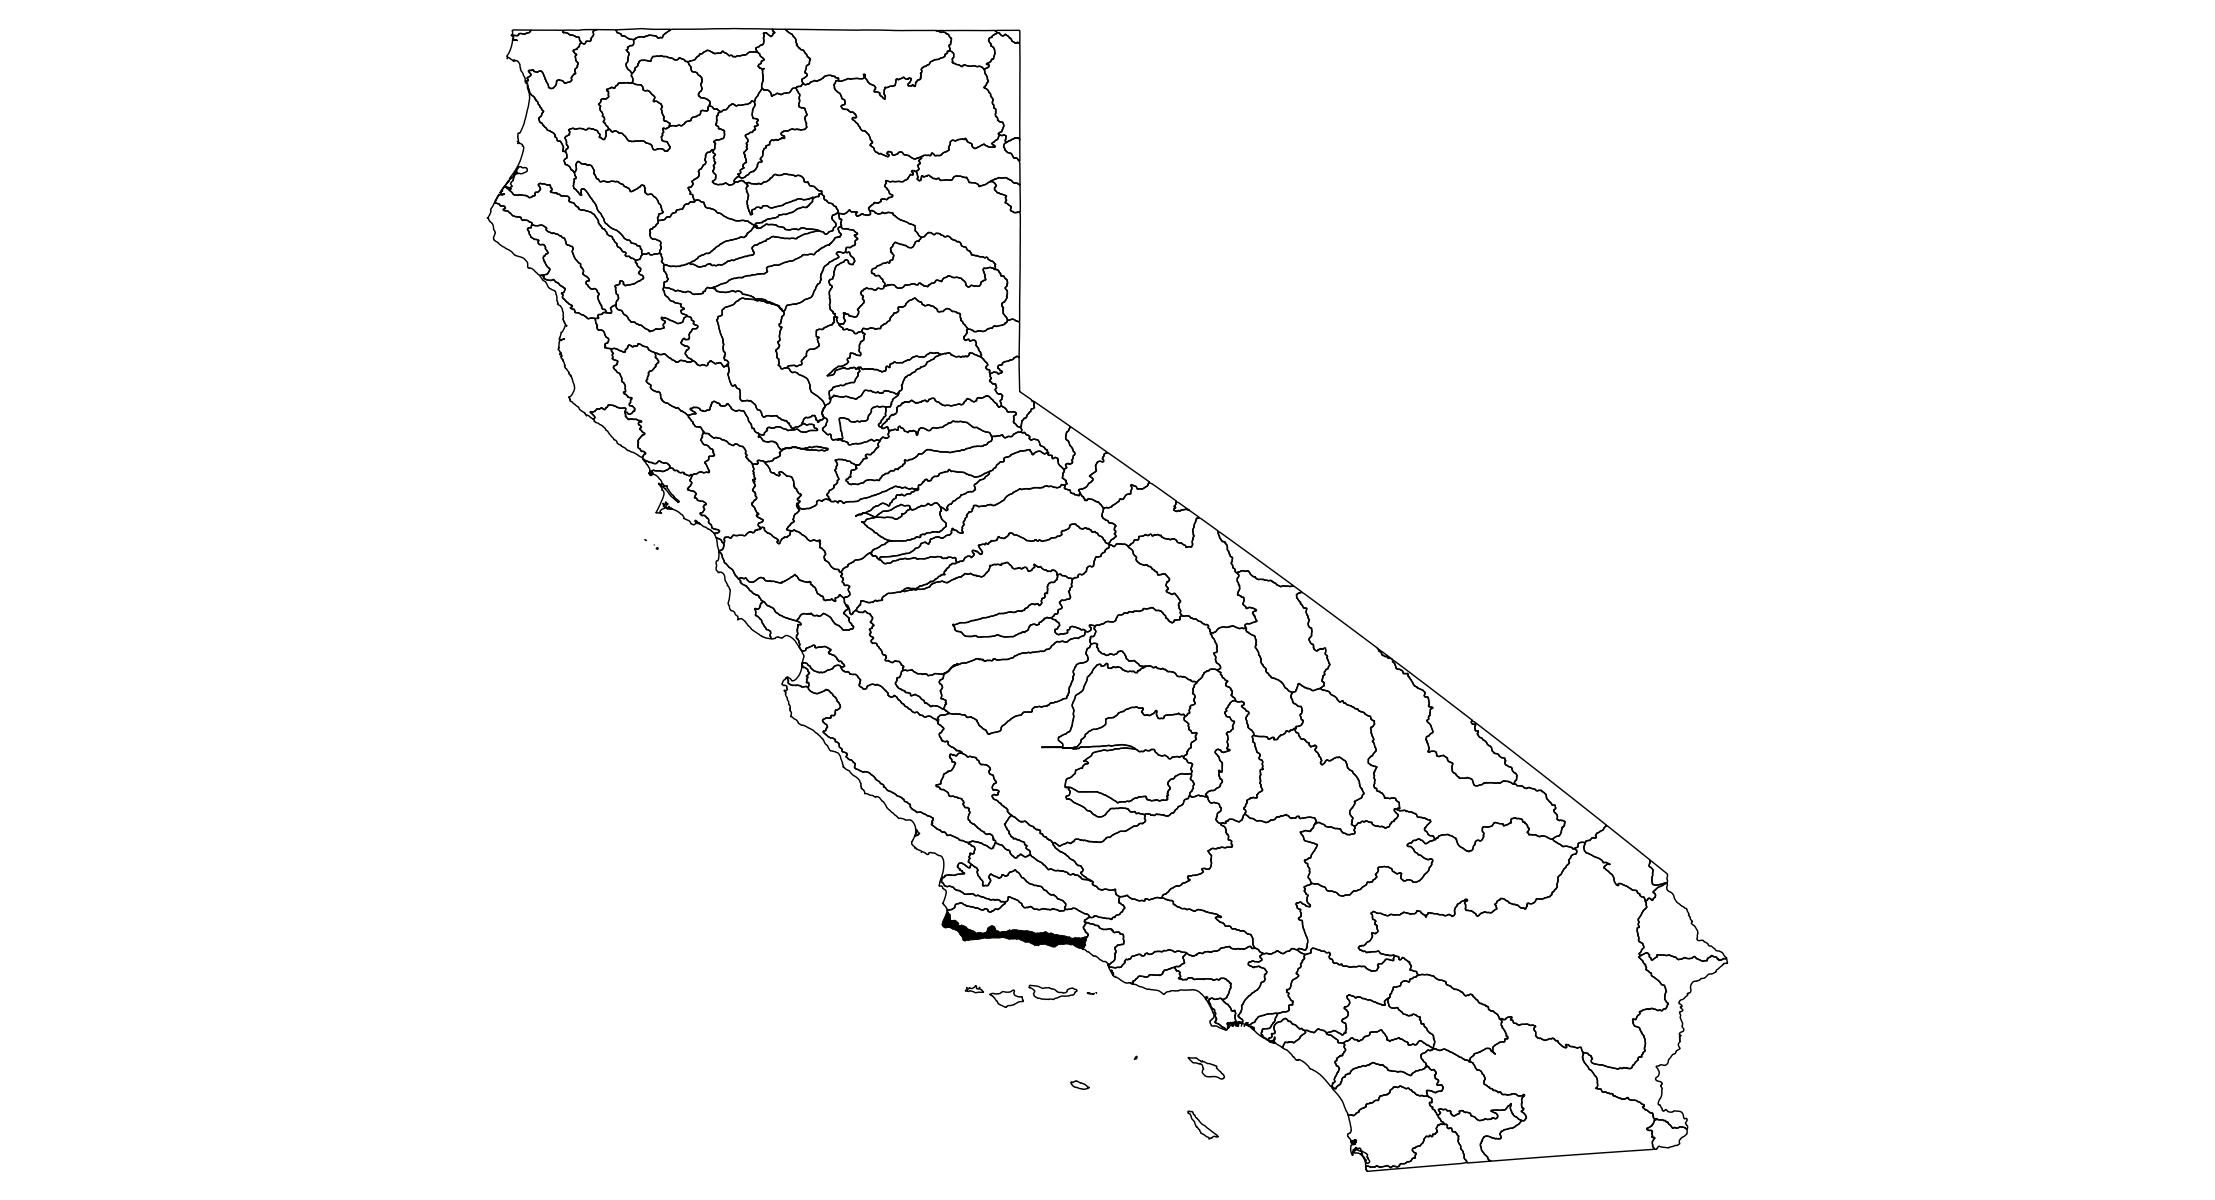
\includegraphics[width=5.5in]{figures/SantaBarbara_Overview.png}   
            \caption{Santa Barbara Region Overview (Filled in Black)}
            \label{fig:SBoverview}
            \end{center}
        \end{figure}

    \subsection{Search Domain}
    
    \begin{itemize}
      \setlength{\itemsep}{0cm}
      \setlength{\parskip}{0cm}
        \item Grid Dimensions: $363$ $cells$ x $1351$ $cells$
        \item Grid Cell Resolution: $100$ $m$ x $100$ $m$ ($1$ $ha$)
        \item Feasible Grid Cells: $117,363$ $cells$
    \end{itemize}
    
        \begin{figure}[!h]
            \begin{center}
            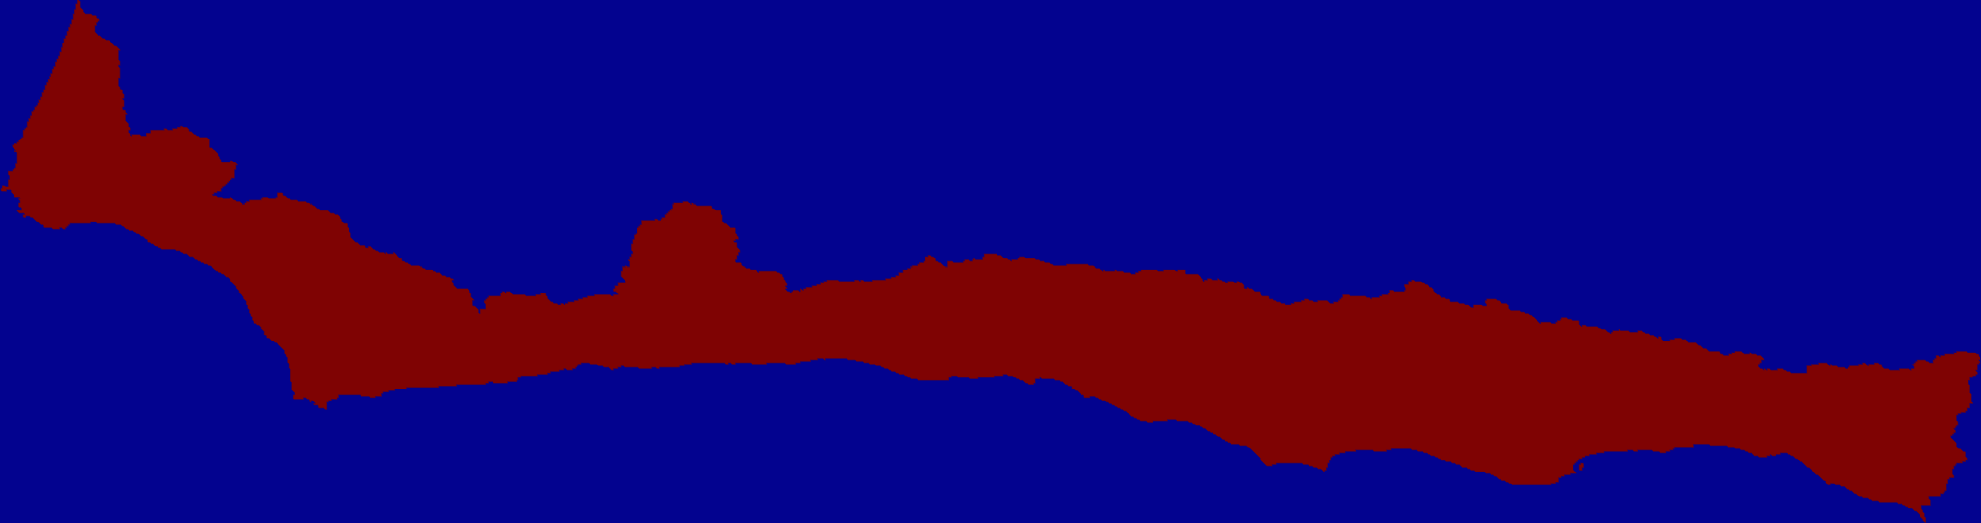
\includegraphics[width=5.5in]{figures/SantaBarbara_SearchDomain.png}   
            \caption{Santa Barbara Region Search Domain (Filled in Red)}
            \label{fig:SBdomain}
            \end{center}
        \end{figure}
        
    \subsection{Destination Search Inputs}
    
        \begin{figure}[!h]
            \begin{center}
            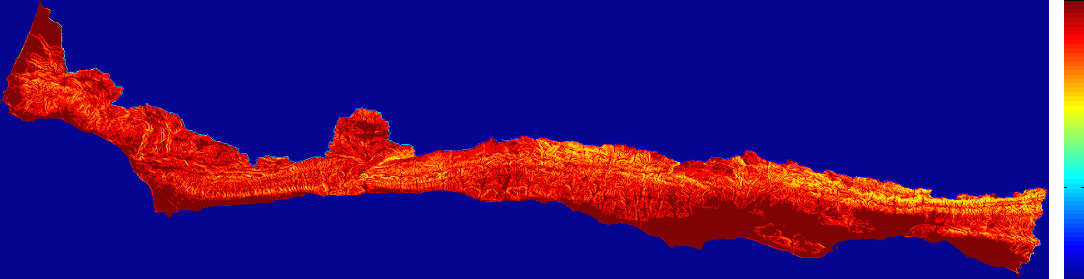
\includegraphics[width=5.5in]{figures/SantaBarbara_Search_Slope.png}   
            \caption{Santa Barbara Region Destination Search Inputs: Slope Score (Blue:Low, Red:High)}
            \label{fig:SBdsinputs_slope}
            \end{center}
        \end{figure}
        
        \begin{figure}[!h]
            \begin{center}
            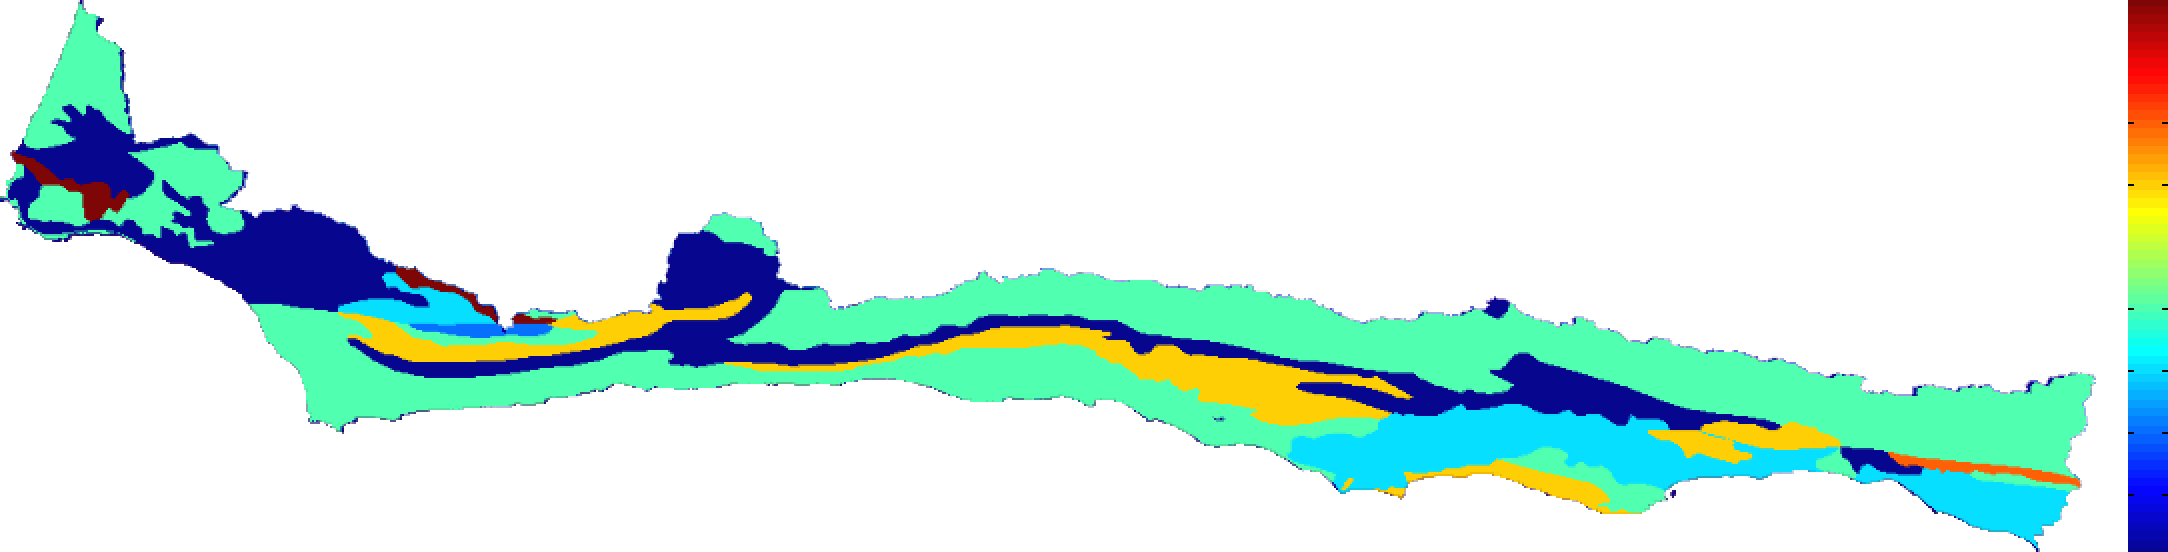
\includegraphics[width=5.5in]{figures/SantaBarbara_Search_Geology.png}   
            \caption{Santa Barbara Region Destination Search Inputs: Geology Score (Blue:Low, Red:High)}
            \label{fig:SBdsinputs_geology}
            \end{center}
        \end{figure}
    
        \begin{figure}[!h]
            \begin{center}
            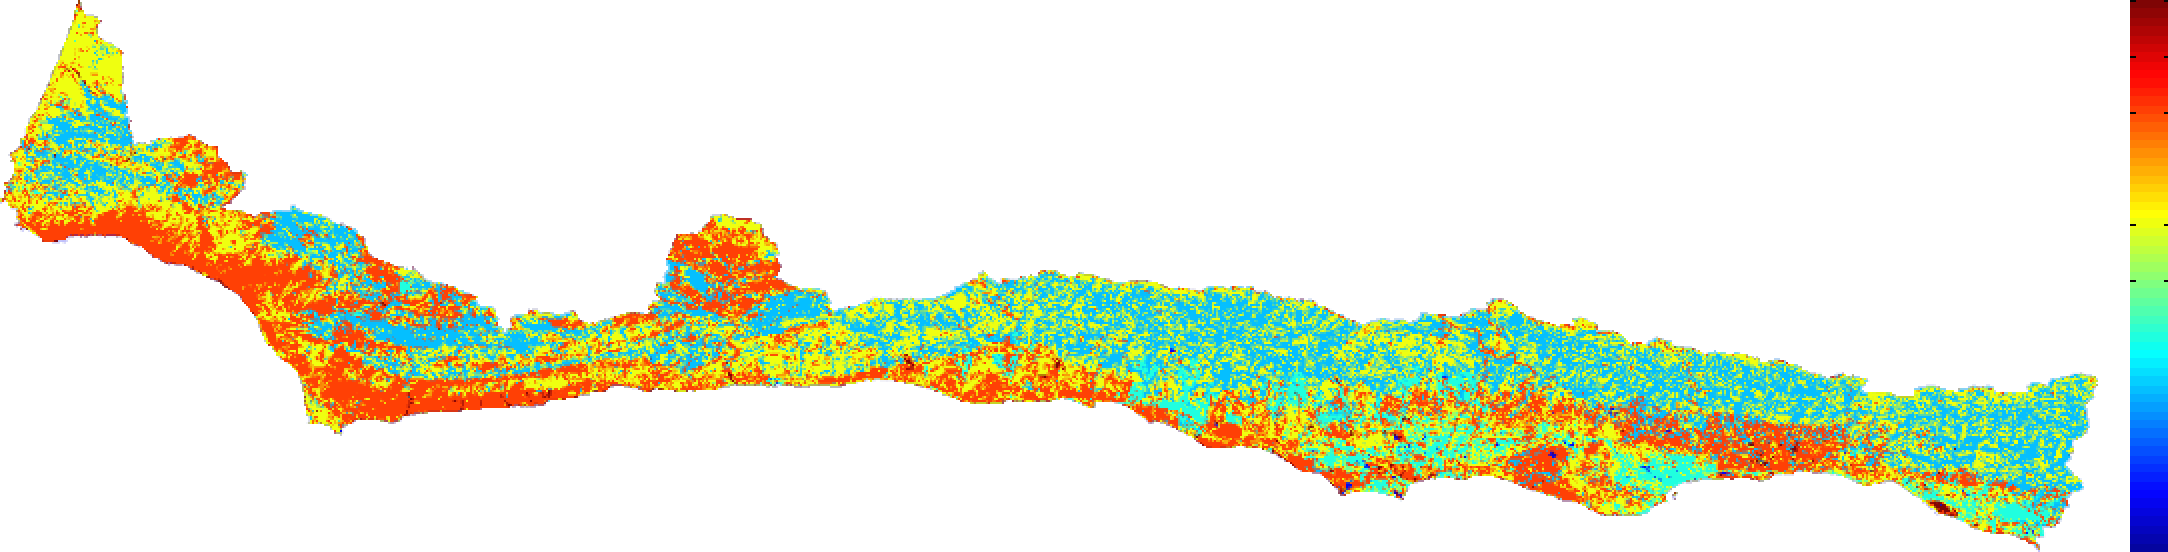
\includegraphics[width=5.5in]{figures/SantaBarbara_Search_Landuse.png}   
            \caption{Santa Barbara Region Destination Search Inputs: Landuse Score (Blue:Low, Red:High)}
            \label{fig:SBdsinputs_landuse}
            \end{center}
        \end{figure}
    
    \subsection{Destination Search Outputs}
    
        \begin{figure}[!h]
            \begin{center}
            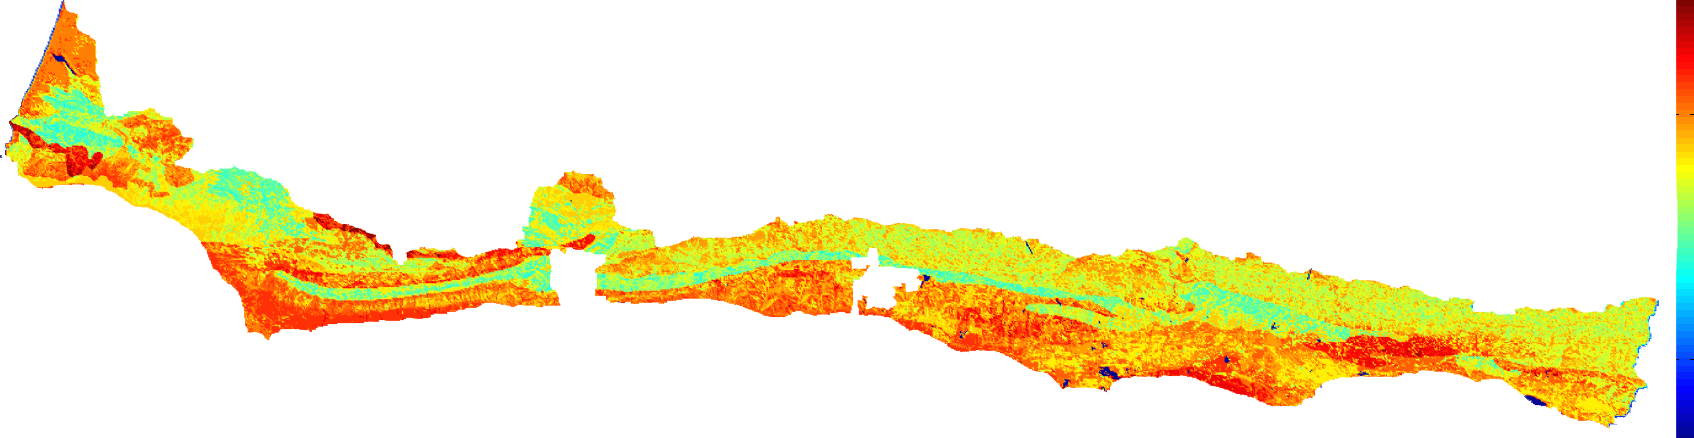
\includegraphics[width=5.5in]{figures/SantaBarbara_Search_Composite.png}   
            \caption{Santa Barbara Region Destination Search Outputs: Composite Scores (Blue:Low, Red:High)}
            \label{fig:SBdsoutputs_comp}
            \end{center}
        \end{figure}
        
        \begin{figure}[!h]
            \begin{center}
            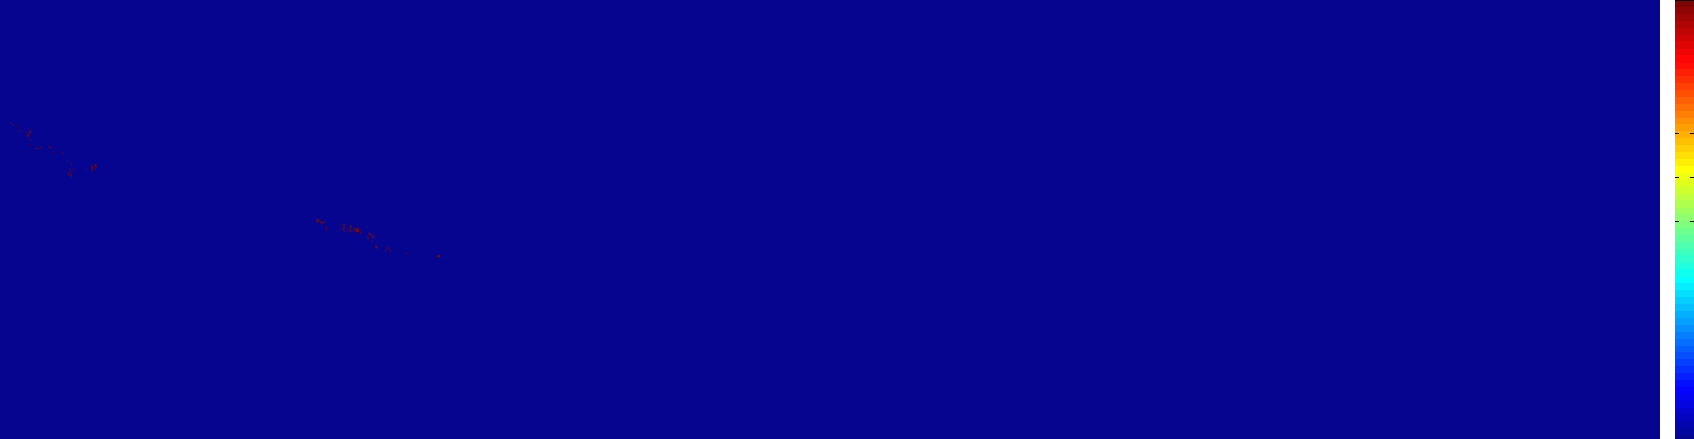
\includegraphics[width=5.5in]{figures/SantaBarbara_Search_Output.png}   
            \caption{Santa Barbara Region Destination Search Outputs: Candidate Regions}
            \label{fig:SBdsoutputs_cand}
            \end{center}
        \end{figure}

    \subsection{Proposed Corridor Endpoints}
    
    \begin{itemize}
      \setlength{\itemsep}{0cm}
      \setlength{\parskip}{0cm}
        \item Start Location: $(313,1083)$
        \item End Destination:    
        \item Shortest Euclidean Path Distance: 
    \end{itemize}
    
        \begin{figure}[!h]
            \begin{center}
            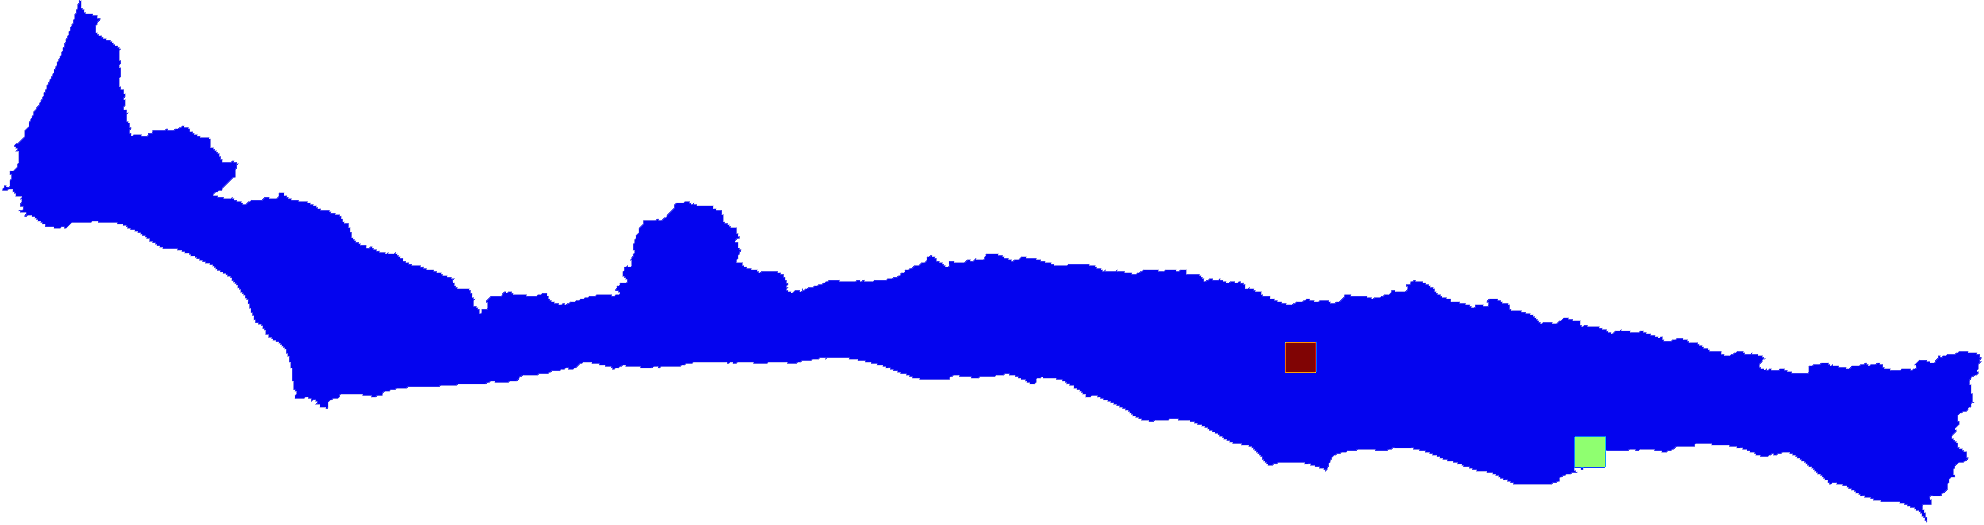
\includegraphics[width=5.5in]{figures/SantaBarbara_Endpoints.png}   
            \caption{Santa Barbara Region Proposed Corridor Endpoints}
            \label{fig:SBendpoints}
            \end{center}
        \end{figure}
            
    \subsection{Proposed Objective Layers}

        \begin{figure}[!h]
            \begin{center}
            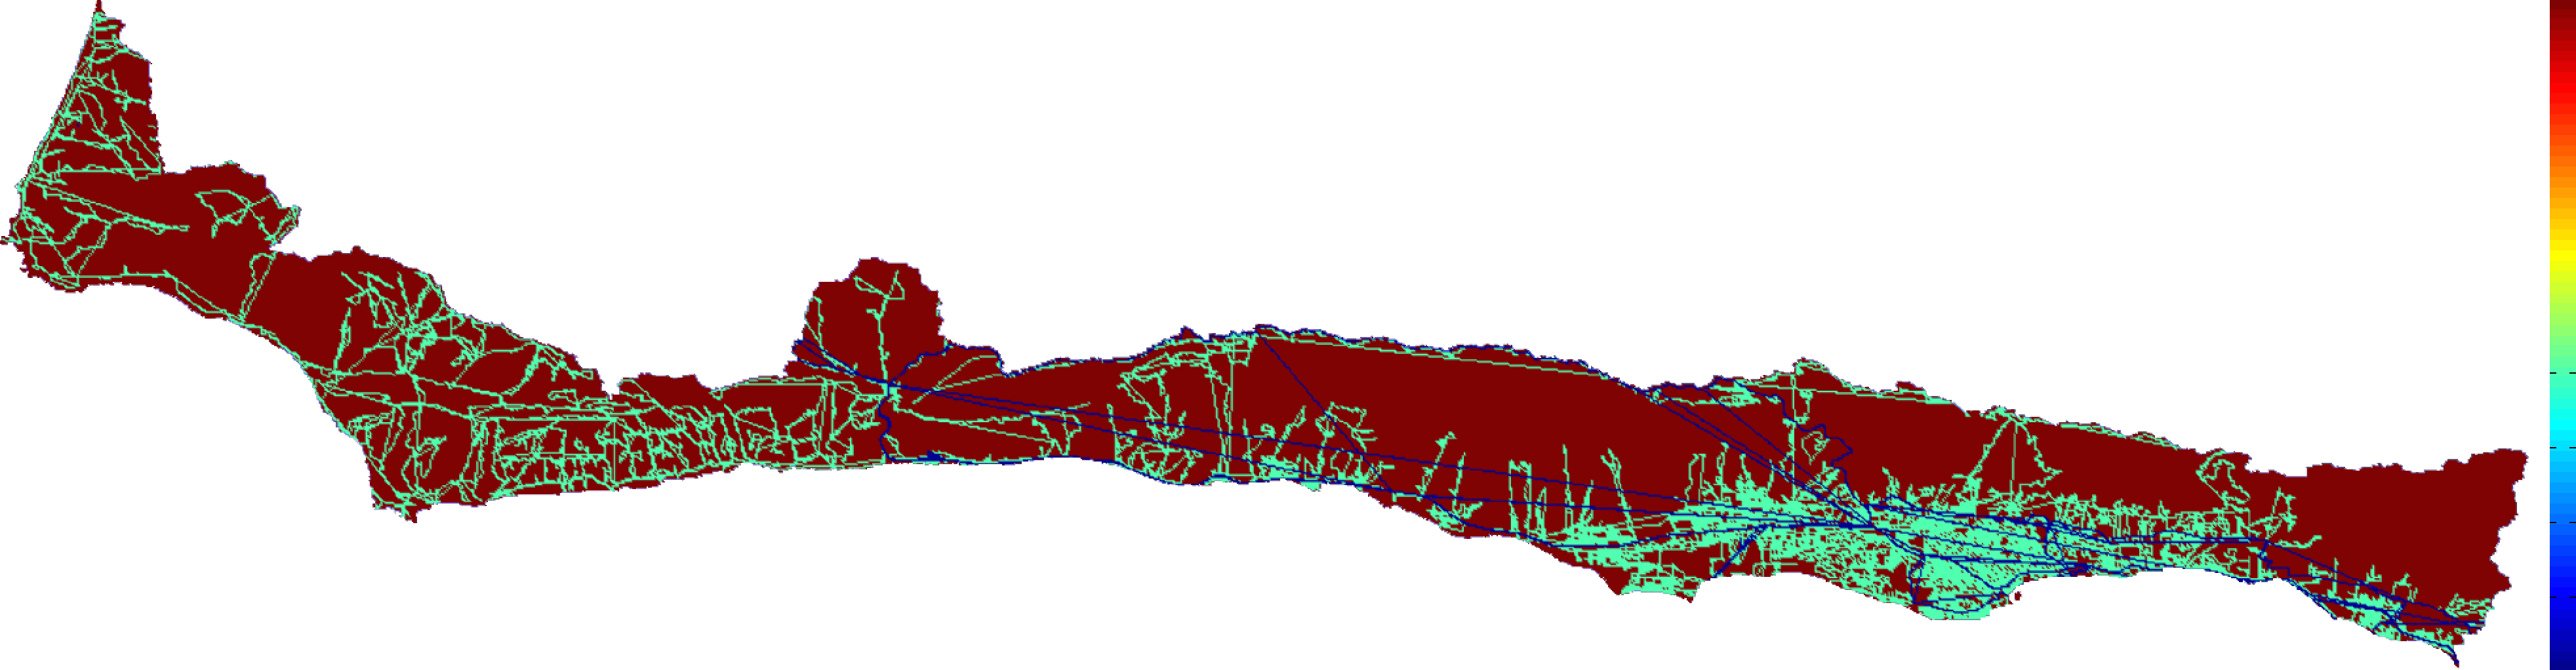
\includegraphics[width=5.5in]{figures/SantaBarbara_AccessibilityScore.png}   
            \caption{Santa Barbara Region Accessibility Based Objective Scores (Blue:Low, Red:High)}
            \label{fig:SBaccessibilty}
            \end{center}
        \end{figure}

        \begin{figure}[!h]
            \begin{center}
            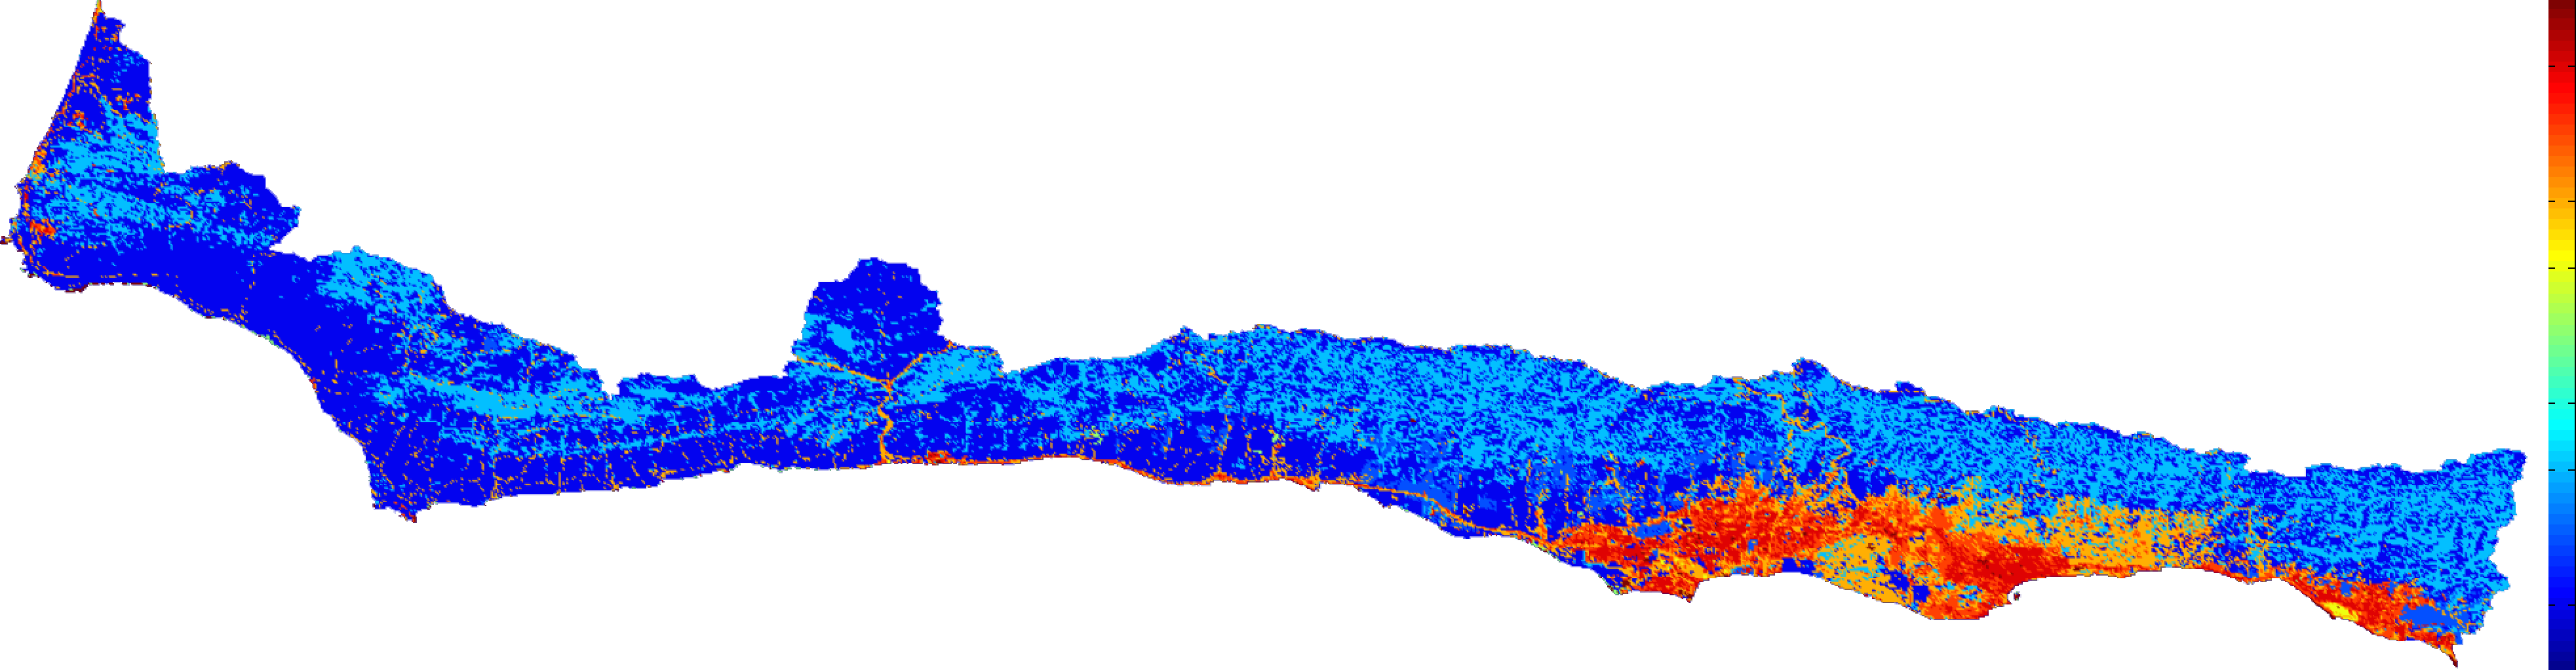
\includegraphics[width=5.5in]{figures/SantaBarbara_DisturbanceScore.png}   
            \caption{Santa Barbara Region Land Use Disturbance Based Objective Scores (Blue:Low, Red:High)}
            \label{fig:SBdisturbance}
            \end{center}
        \end{figure}
        
        \begin{figure}[!h]
            \begin{center}
            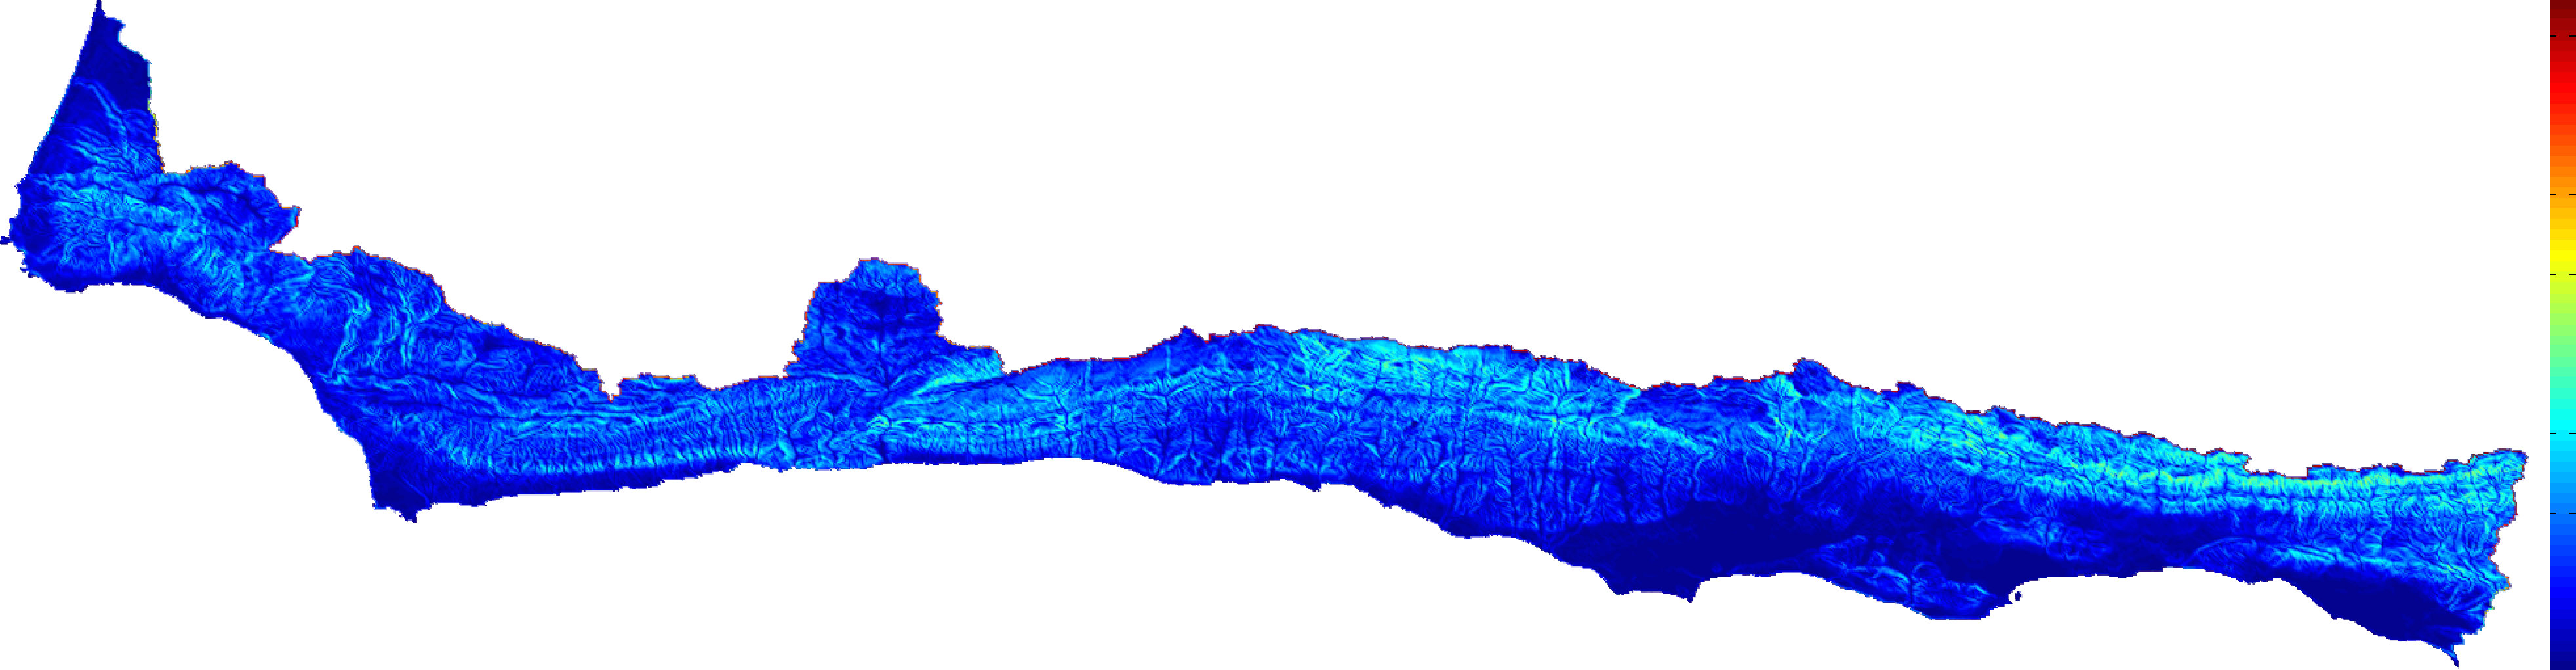
\includegraphics[width=5.5in]{figures/SantaBarbara_SlopeScore.png}   
            \caption{Santa Barbara Region Slope Based Objective Scores (Blue:Low, Red:High)}
            \label{fig:SBslope}
            \end{center}
        \end{figure}
        
    \subsection{Proposed Corridor Solutions}
    
        \begin{figure}[!h]
            \begin{center}
            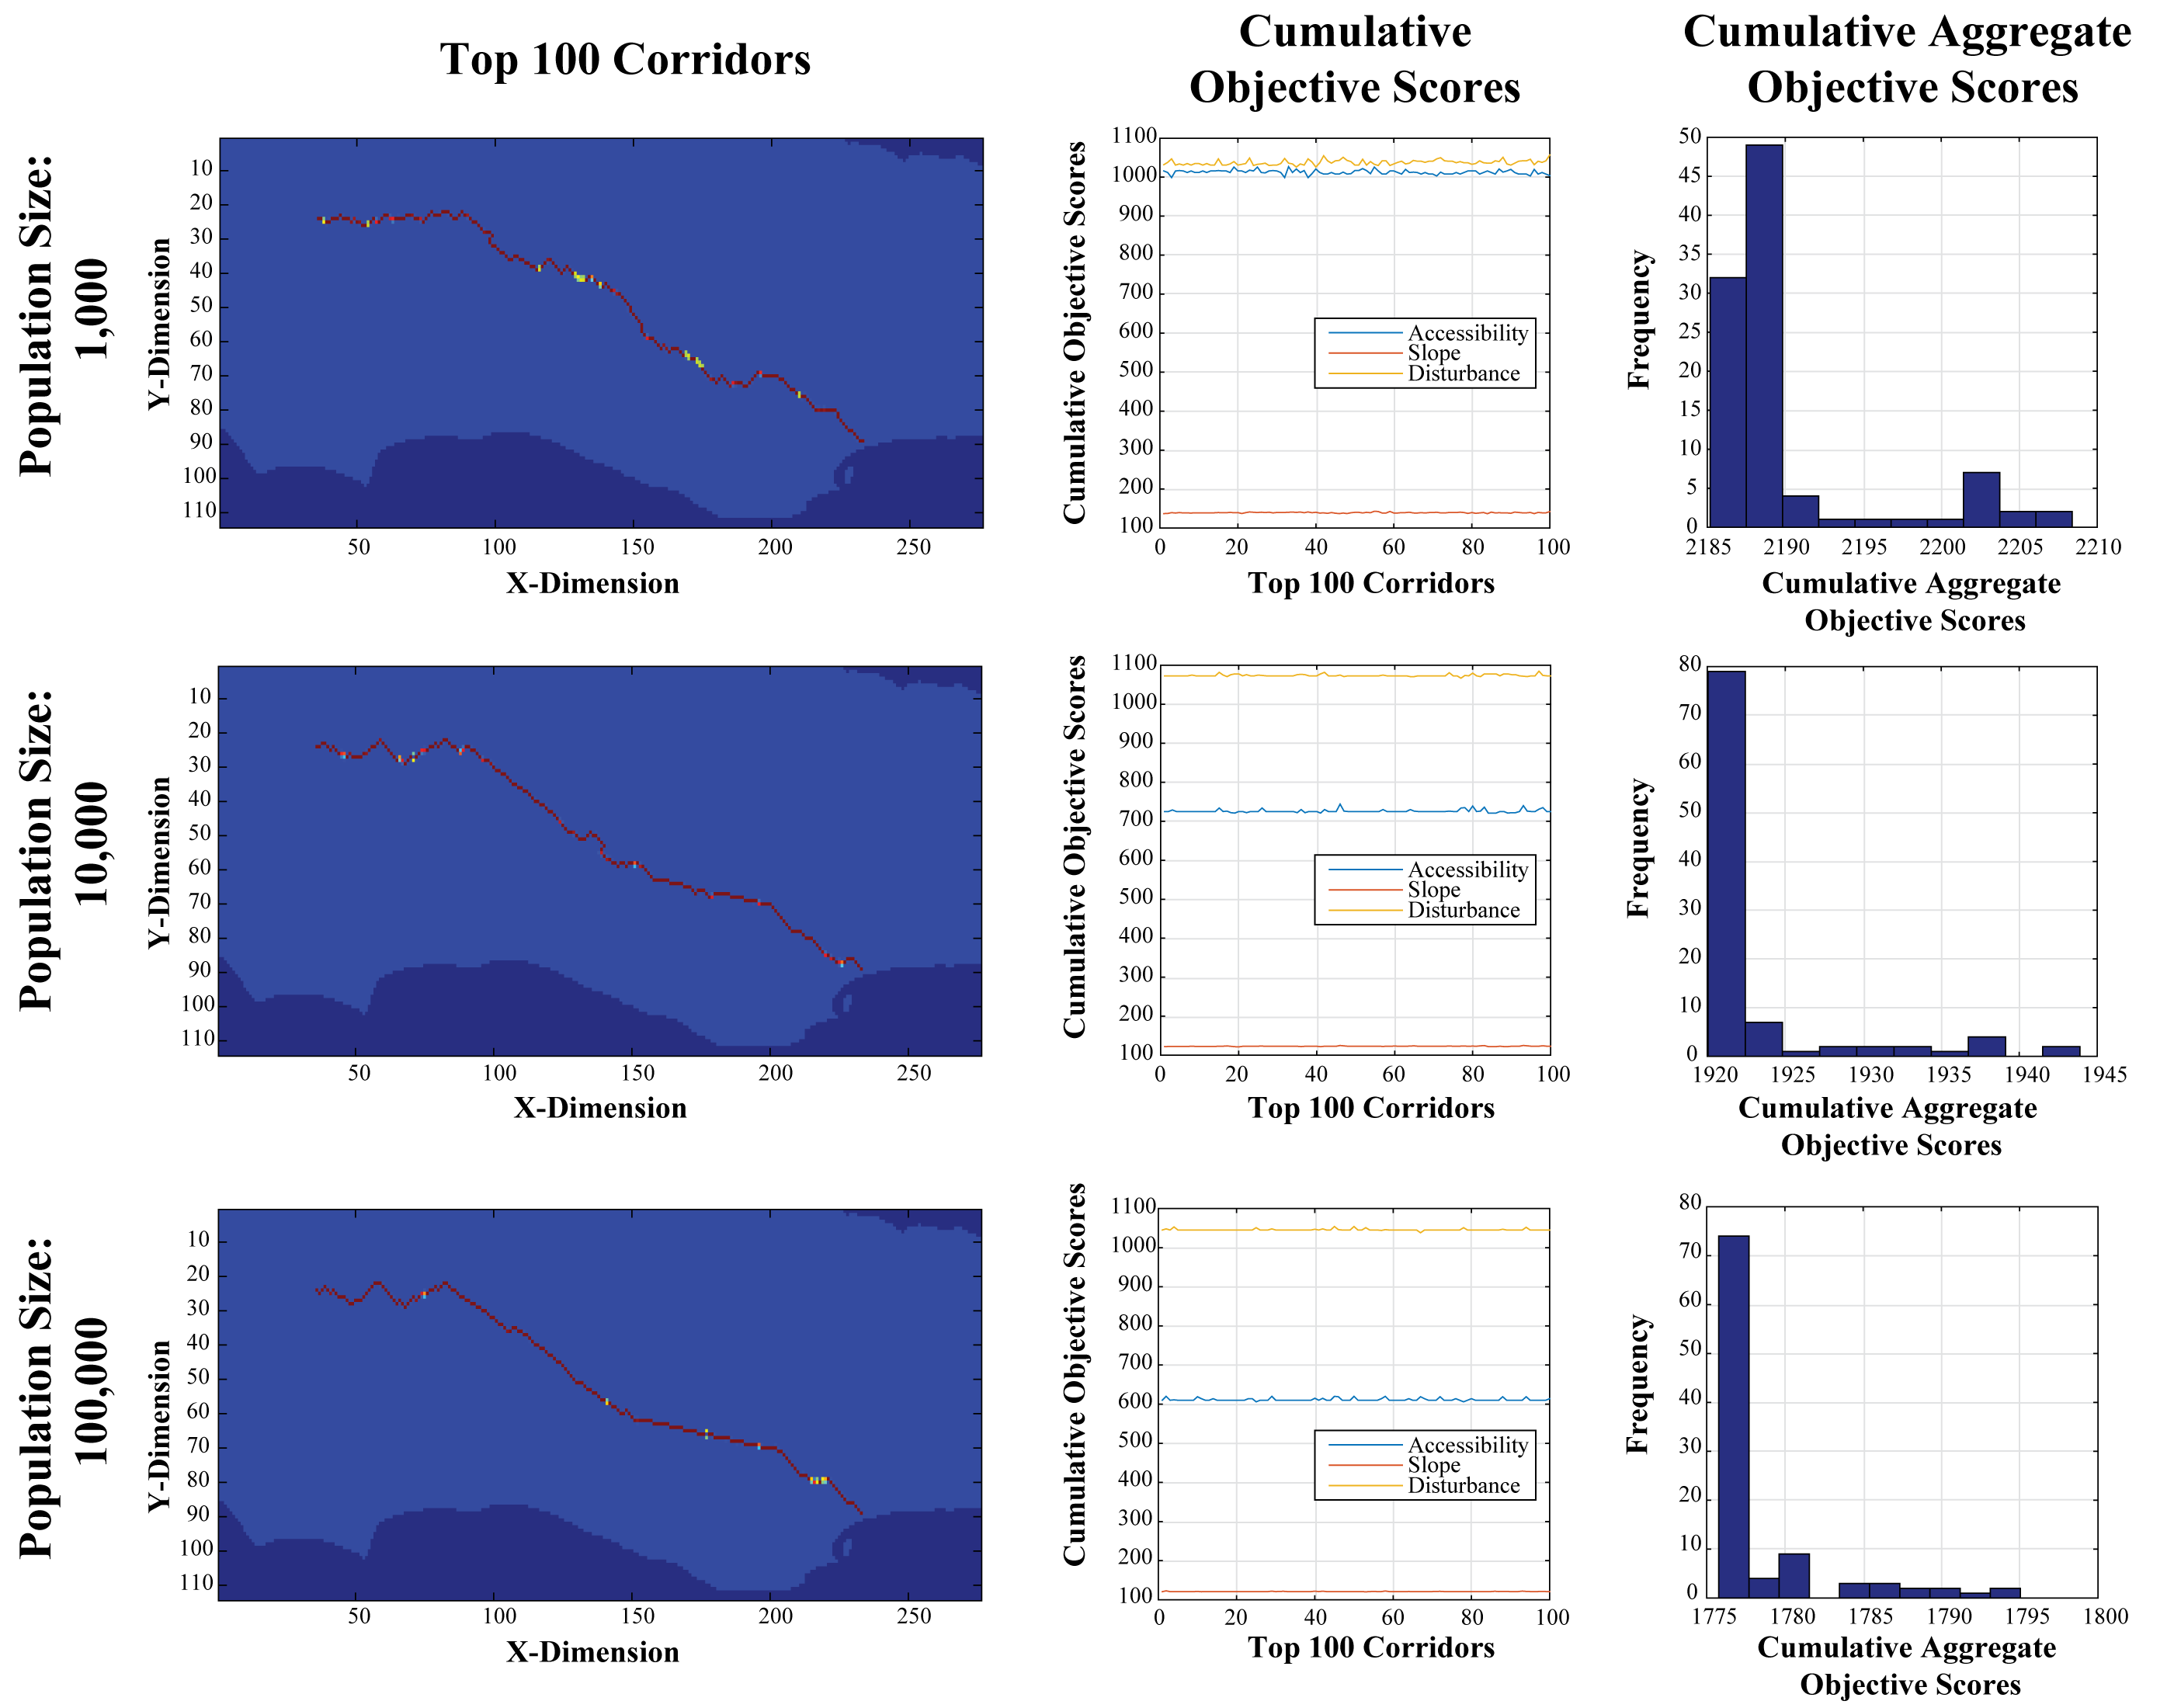
\includegraphics[width=6in]{figures/SantaBarbara_PathwayResults.png}   
            \caption{Santa Barbara Region Corridor Analysis Results}
            \label{fig:SBresults}
            \end{center}
        \end{figure}

        \begin{figure}[!h]
            \begin{center}
            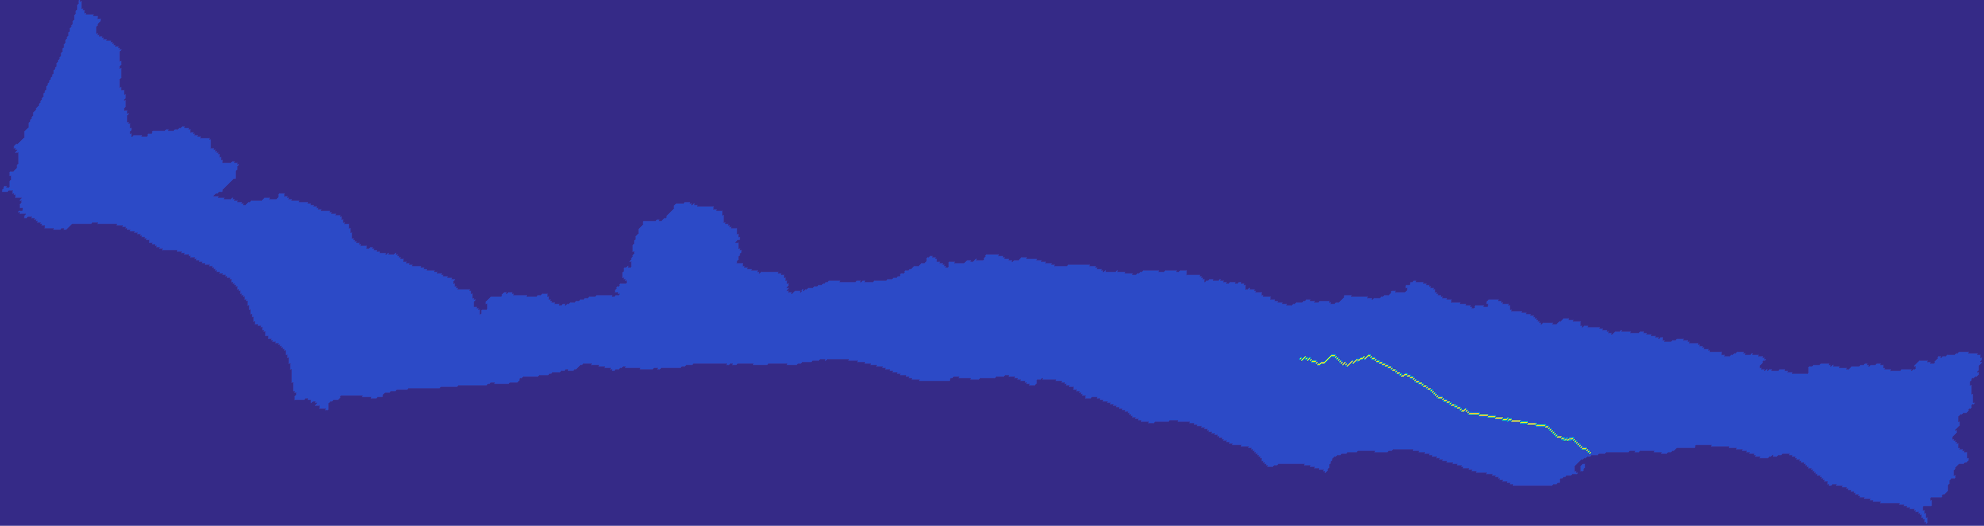
\includegraphics[width=5.5in]{figures/SantaBarbara_PathwayLarge.png}   
            \caption{Santa Barbara Region Top 100 Corridors (Pop Size: 100,000) Basin Wide Overview}
            \label{fig:SBsolutionOverview}
            \end{center}
        \end{figure}
        
    \subsection{Anticipated Distribution of Life Cycle Energy Usages and Net Water Savings}
    
\section{Oxnard Region}

    \subsection{Regional Context}
    
    \begin{itemize}
      \setlength{\itemsep}{0cm}
      \setlength{\parskip}{0cm}
        \item HUC-8 Code: $18070102$
        \item Total Area: $5,188.3$ $km^2$
        \item Maximum Elevation: $2,664.4$ $m$
        \item Minimum Elevation: $-0.05$ $m$
        \item Mean Slope: $15.54$ $\%$
        \item Standard Deviation of Slope: $11.11$ $\%$
        \item Dominant Soil Composition: Hydrologic Soil Group - B: $10-20\%$ clay, $50-90\%$ sand, $35\%$ rock fragments
    \end{itemize}
    
        \begin{figure}[!h]
            \begin{center}
            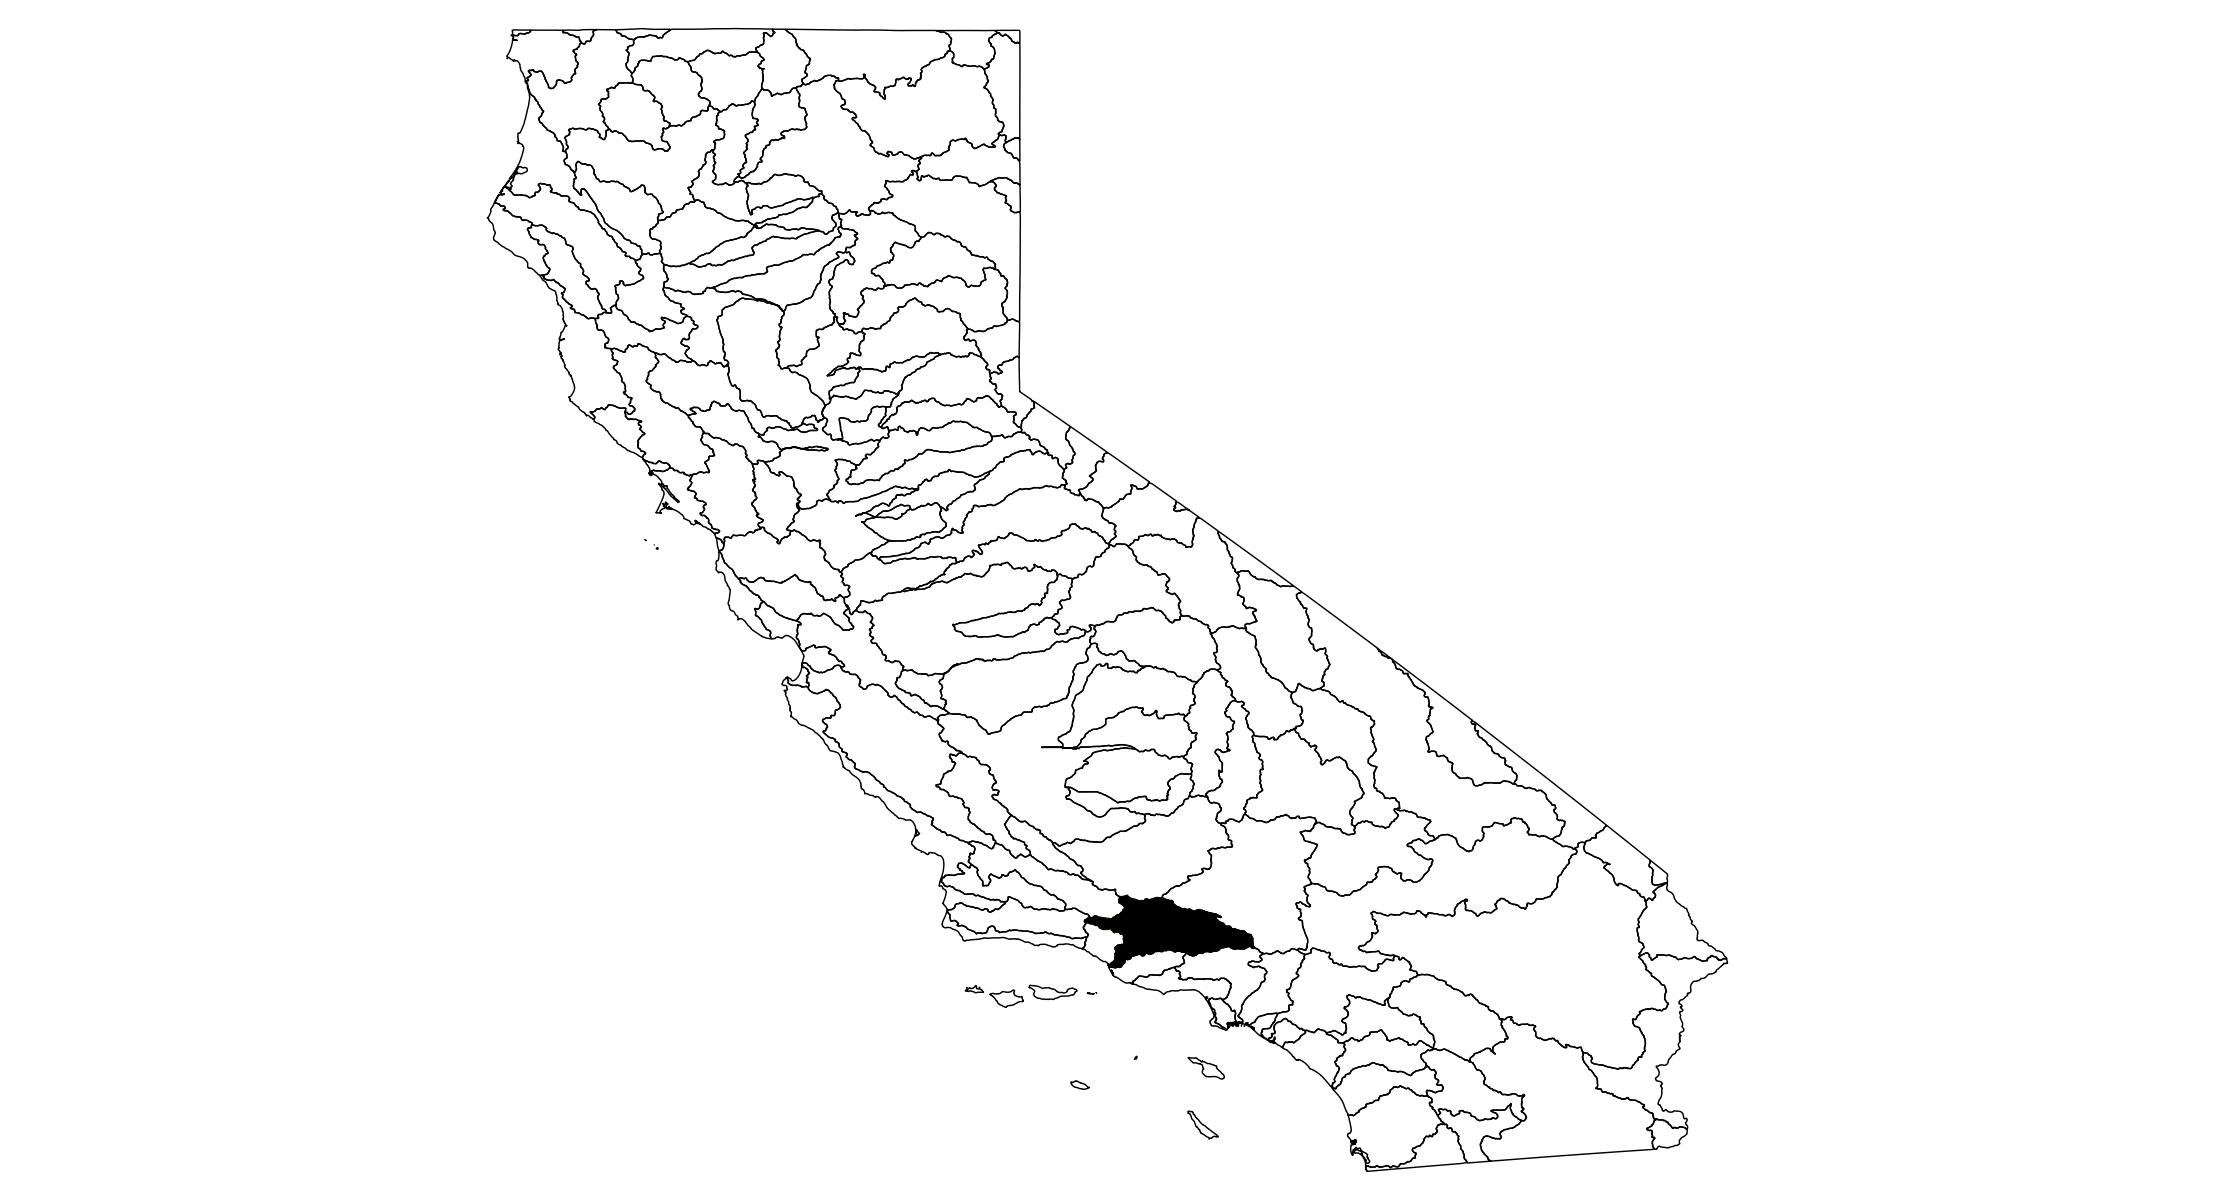
\includegraphics[width=5.5in]{figures/Oxnard_Overview.png}   
            \caption{Oxnard Region Overview (Filled in Black)}
            \label{fig:Ooverview}
            \end{center}
        \end{figure}

    \subsection{Search Domain}
    
    \begin{itemize}
      \setlength{\itemsep}{0cm}
      \setlength{\parskip}{0cm}
        \item Grid Dimensions: $677$ $cells$ x $1586$ $cells$
        \item Grid Cell Resolution: $100$ $m$ x $100$ $m$ ($1$ $ha$)
        \item Feasible Grid Cells: $518,834$ $cells$
    \end{itemize}
    
        \begin{figure}[!h]
            \begin{center}
            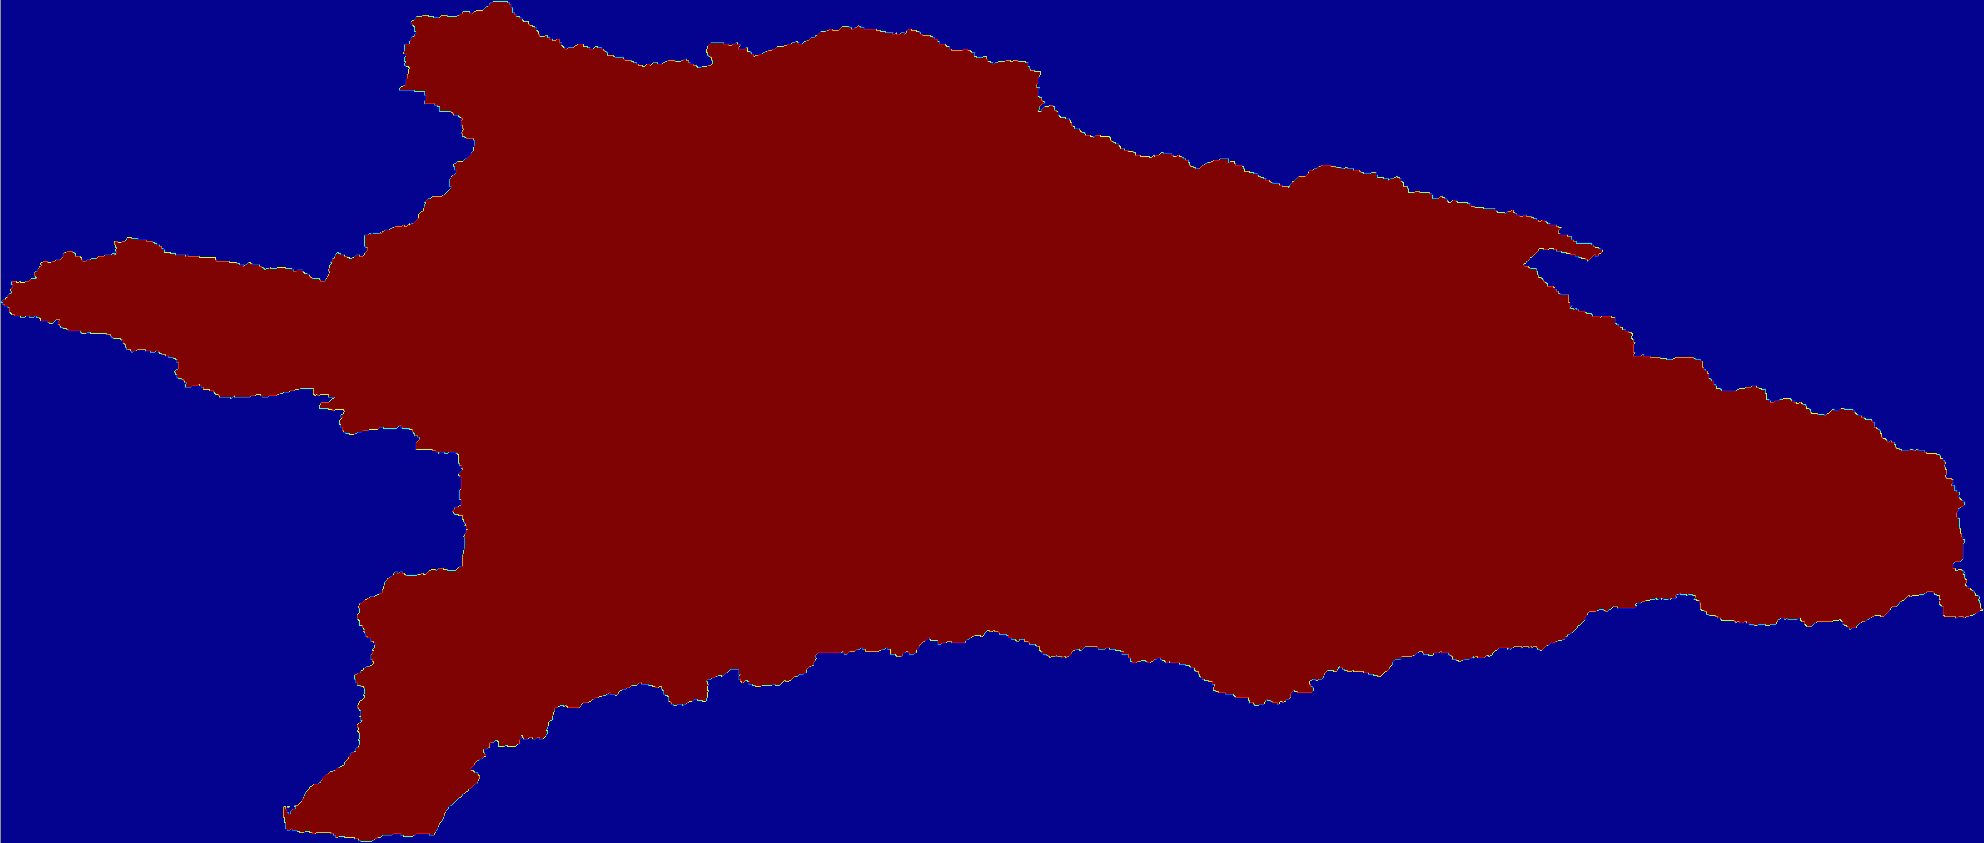
\includegraphics[width=5.5in]{figures/Oxnard_SearchDomain.png}   
            \caption{Oxnard Region Search Domain (Filled in Red)}
            \label{fig:Odomain}
            \end{center}
        \end{figure}
        
    \subsection{Destination Search Inputs}
    
        \begin{figure}[!h]
            \begin{center}
            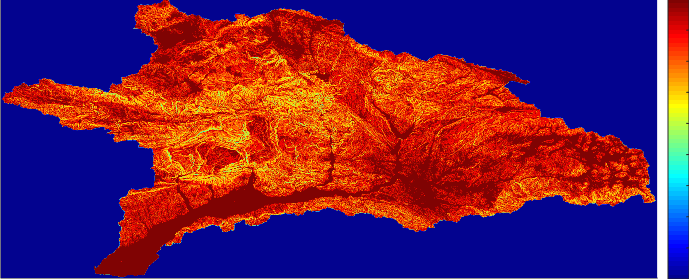
\includegraphics[width=5.5in]{figures/Oxnard_Search_Slope.png}   
            \caption{Oxnard Region Destination Search Inputs: Slope Score (Blue:Low, Red:High)}
            \label{fig:Odsinputs_slope}
            \end{center}
        \end{figure}
        
        \begin{figure}[!h]
            \begin{center}
            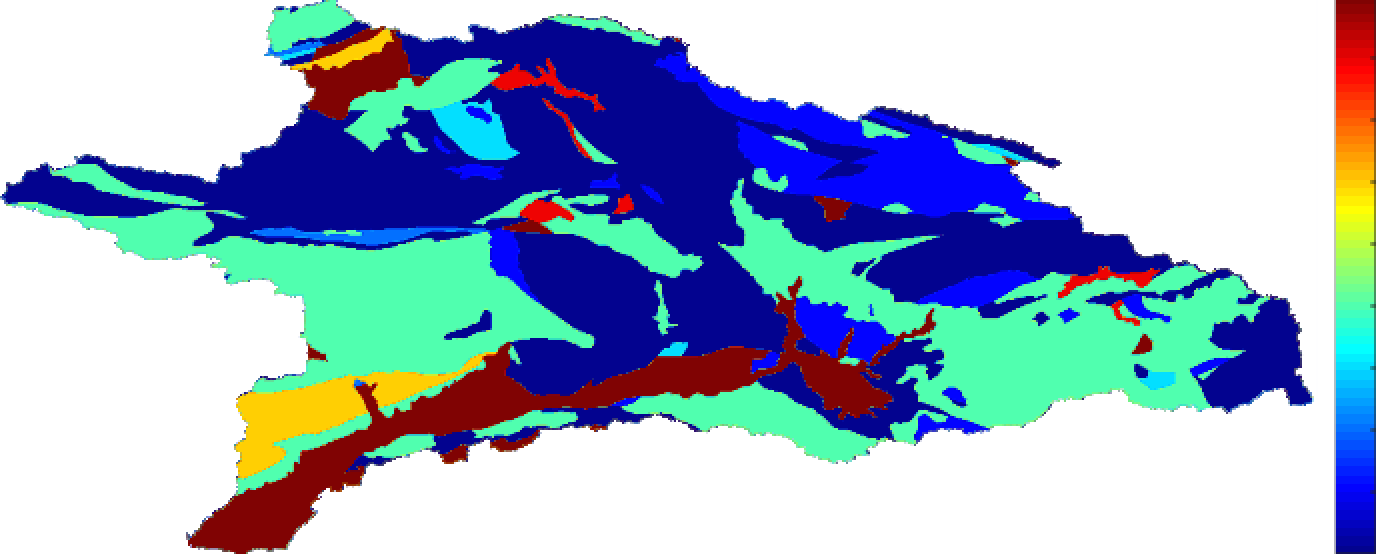
\includegraphics[width=5.5in]{figures/Oxnard_Search_Geology.png}   
            \caption{Oxnard Region Destination Search Inputs: Geology Score (Blue:Low, Red:High)}
            \label{fig:Odsinputs_geology}
            \end{center}
        \end{figure}
    
        \begin{figure}[!h]
            \begin{center}
            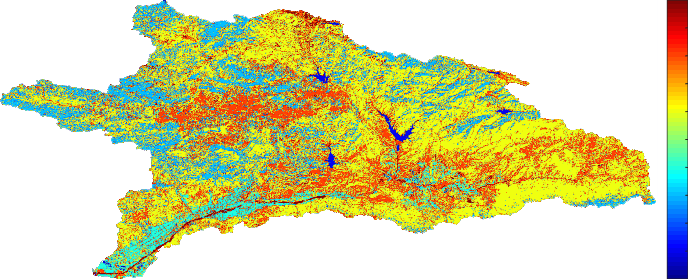
\includegraphics[width=5.5in]{figures/Oxnard_Search_Landuse.png}   
            \caption{Oxnard Region Destination Search Inputs: Landuse Score (Blue:Low, Red:High)}
            \label{fig:Odsinputs_landuse}
            \end{center}
        \end{figure}
    
    \subsection{Destination Search Outputs}
    
        \begin{figure}[!h]
            \begin{center}
            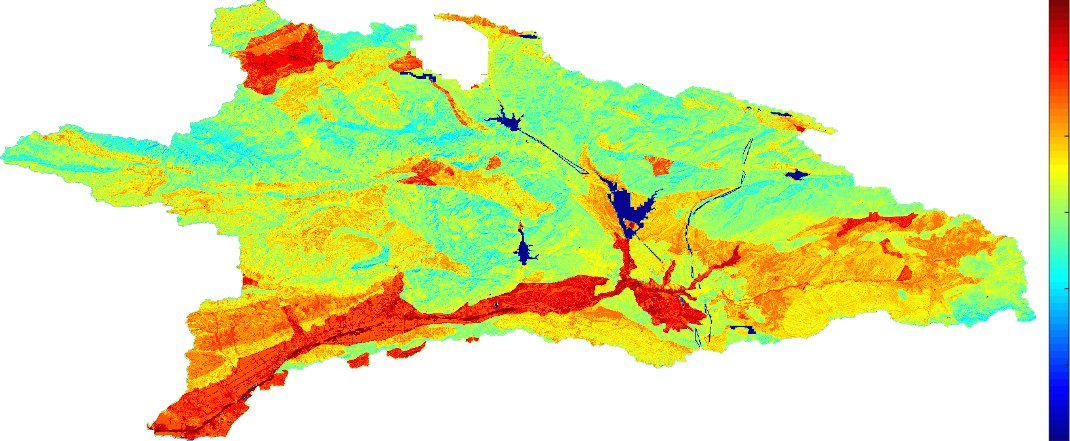
\includegraphics[width=5.5in]{figures/Oxnard_Search_Composite.png}   
            \caption{Oxnard Region Destination Search Outputs: Composite Scores (Blue:Low, Red:High)}
            \label{fig:Odsoutputs_comp}
            \end{center}
        \end{figure}
        
        \begin{figure}[!h]
            \begin{center}
            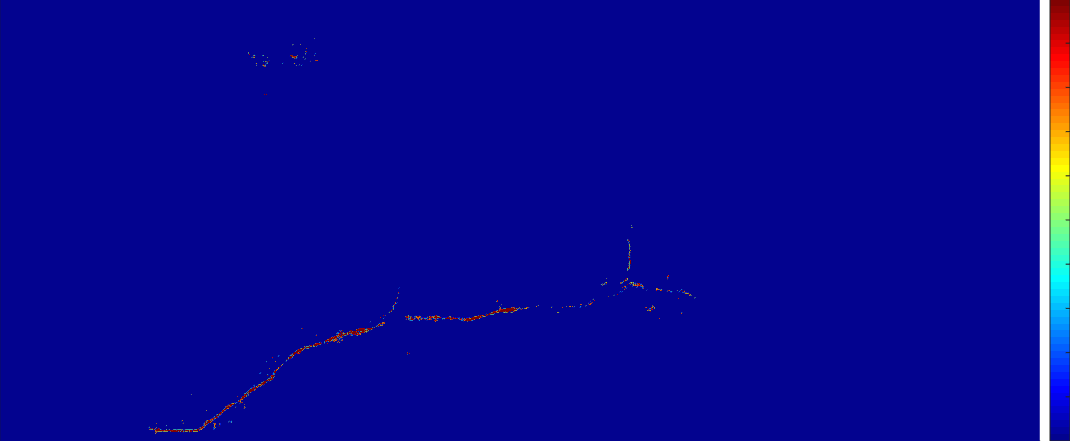
\includegraphics[width=5.5in]{figures/Oxnard_Search_Output.png}   
            \caption{Oxnard Region Destination Search Outputs: Candidate Regions}
            \label{fig:Odsoutputs_cand}
            \end{center}
        \end{figure}

    \subsection{Proposed Corridor Endpoints}
    
    \begin{itemize}
      \setlength{\itemsep}{0cm}
      \setlength{\parskip}{0cm}
        \item Start Location: $(656,236)$
        \item End Destination: $(513,532)$
        \item Shortest Euclidean Path Distance: 
    \end{itemize}
    
        \begin{figure}[!h]
            \begin{center}
            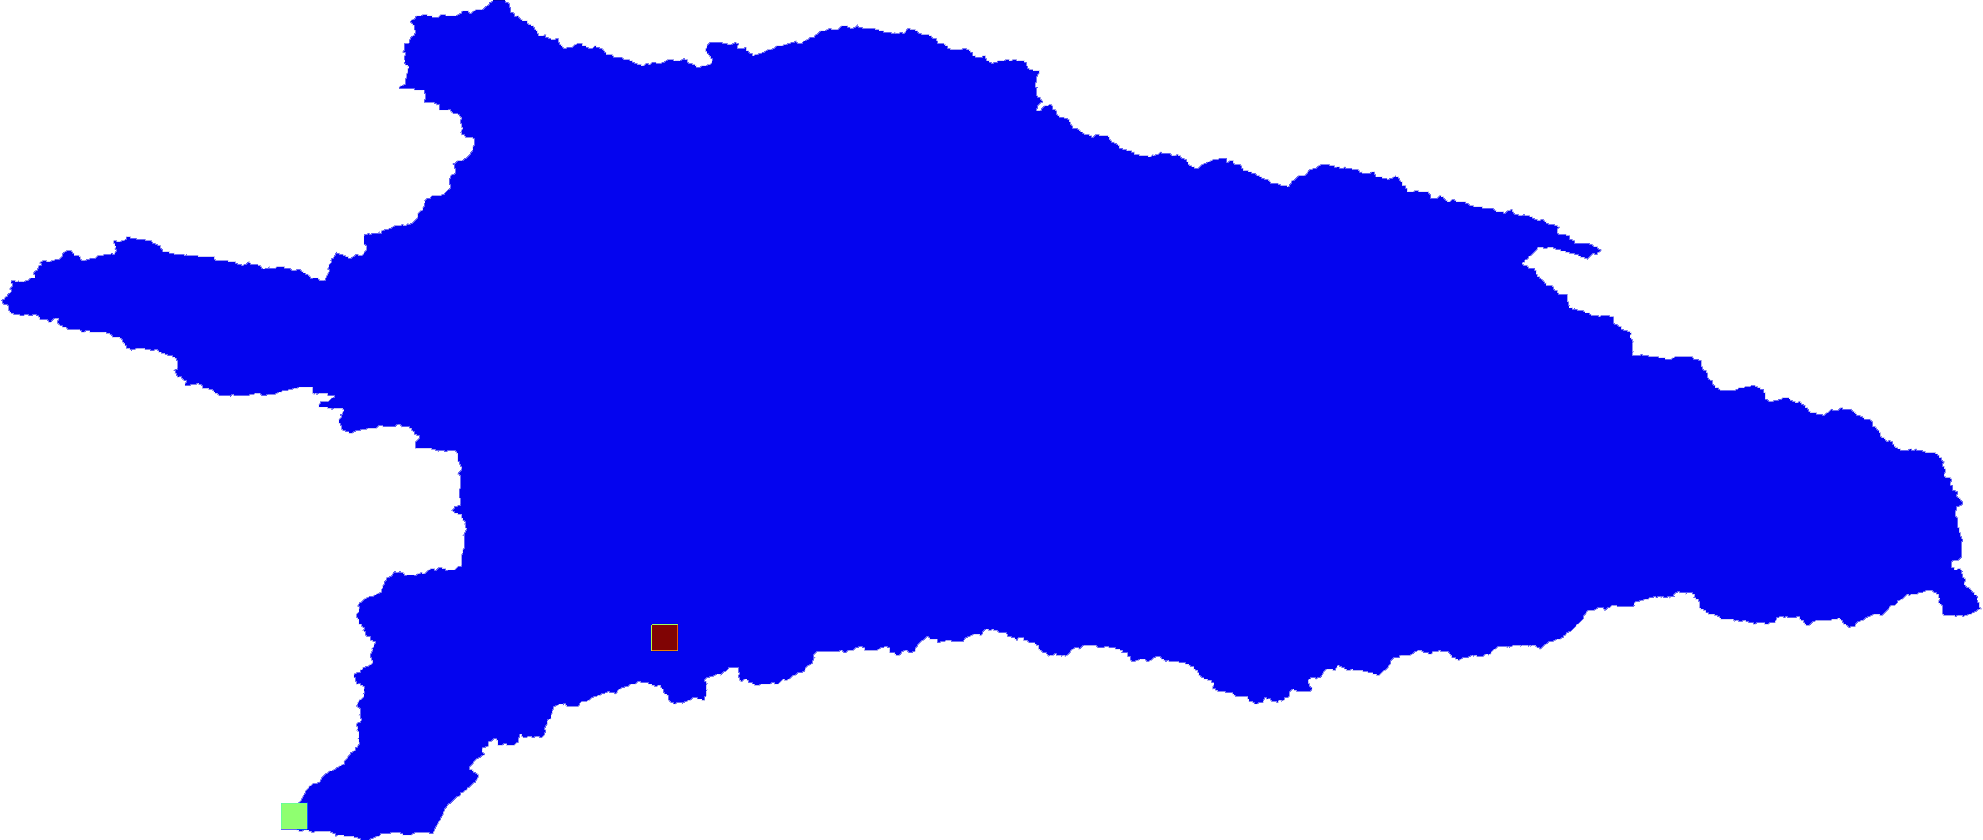
\includegraphics[width=5.5in]{figures/Oxnard_Endpoints.png}   
            \caption{Oxnard Region Proposed Corridor Endpoints}
            \label{fig:Oendpoints}
            \end{center}
        \end{figure}
            
    \subsection{Proposed Objective Layers}

        \begin{figure}[!h]
            \begin{center}
            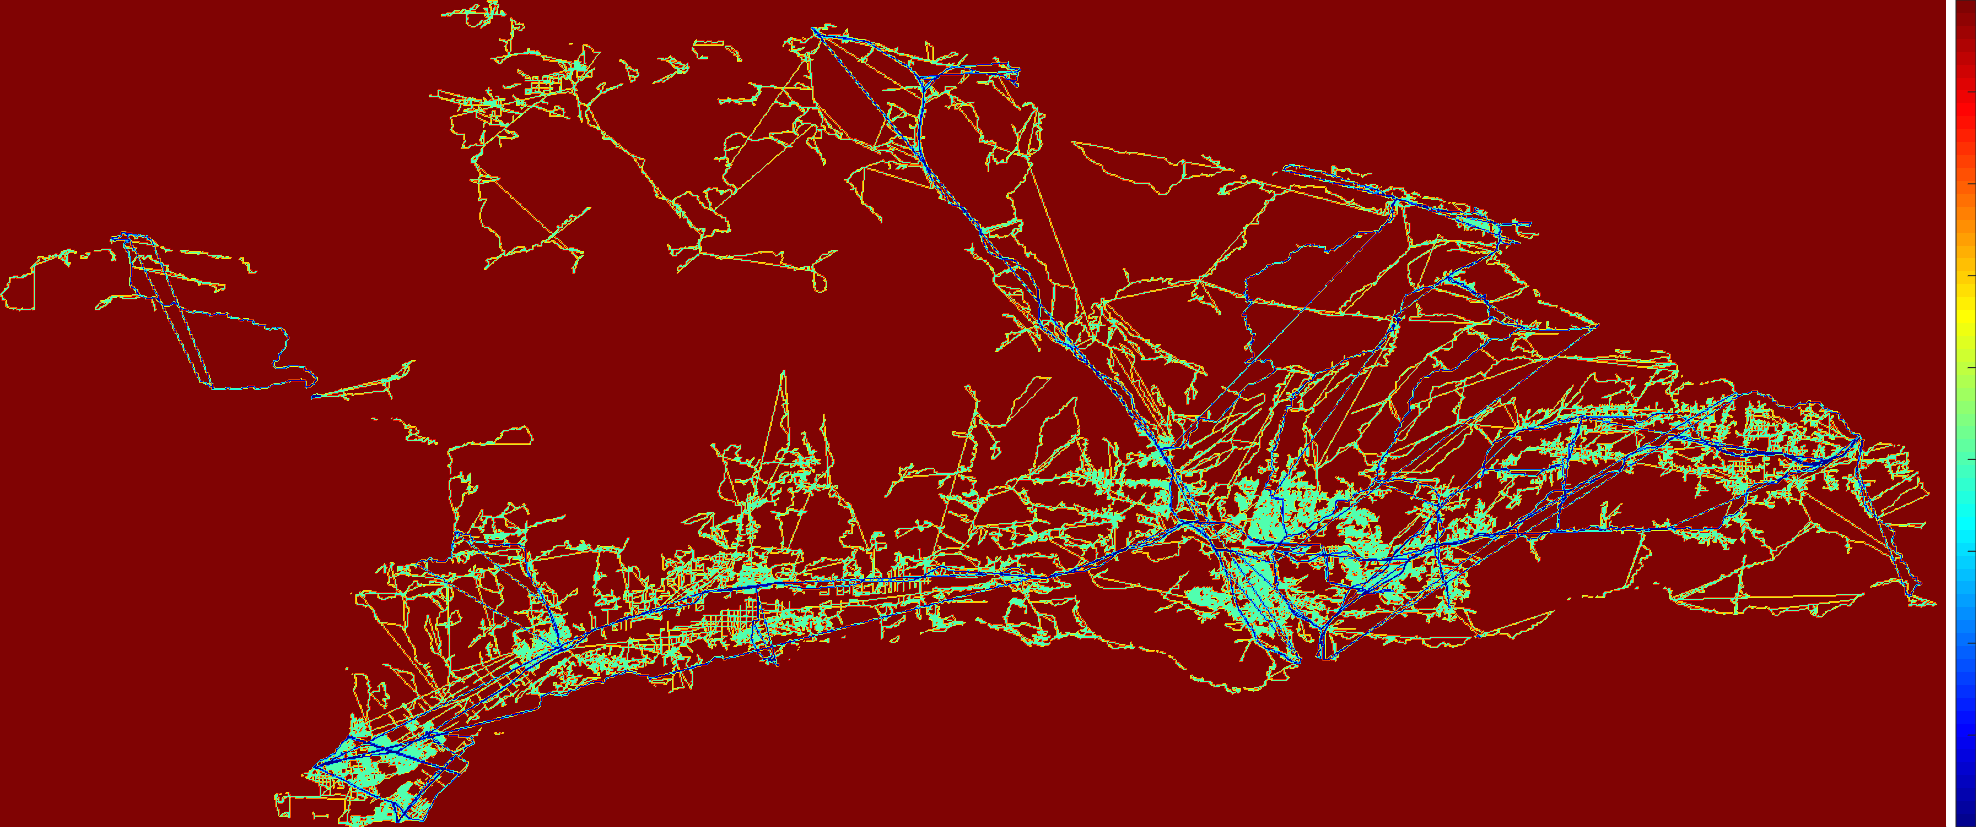
\includegraphics[width=5.5in]{figures/Oxnard_AccessibilityScore.png}   
            \caption{Oxnard Region Accessibility Based Objective Scores (Blue:Low, Red:High)}
            \label{fig:Oaccessibilty}
            \end{center}
        \end{figure}

        \begin{figure}[!h]
            \begin{center}
            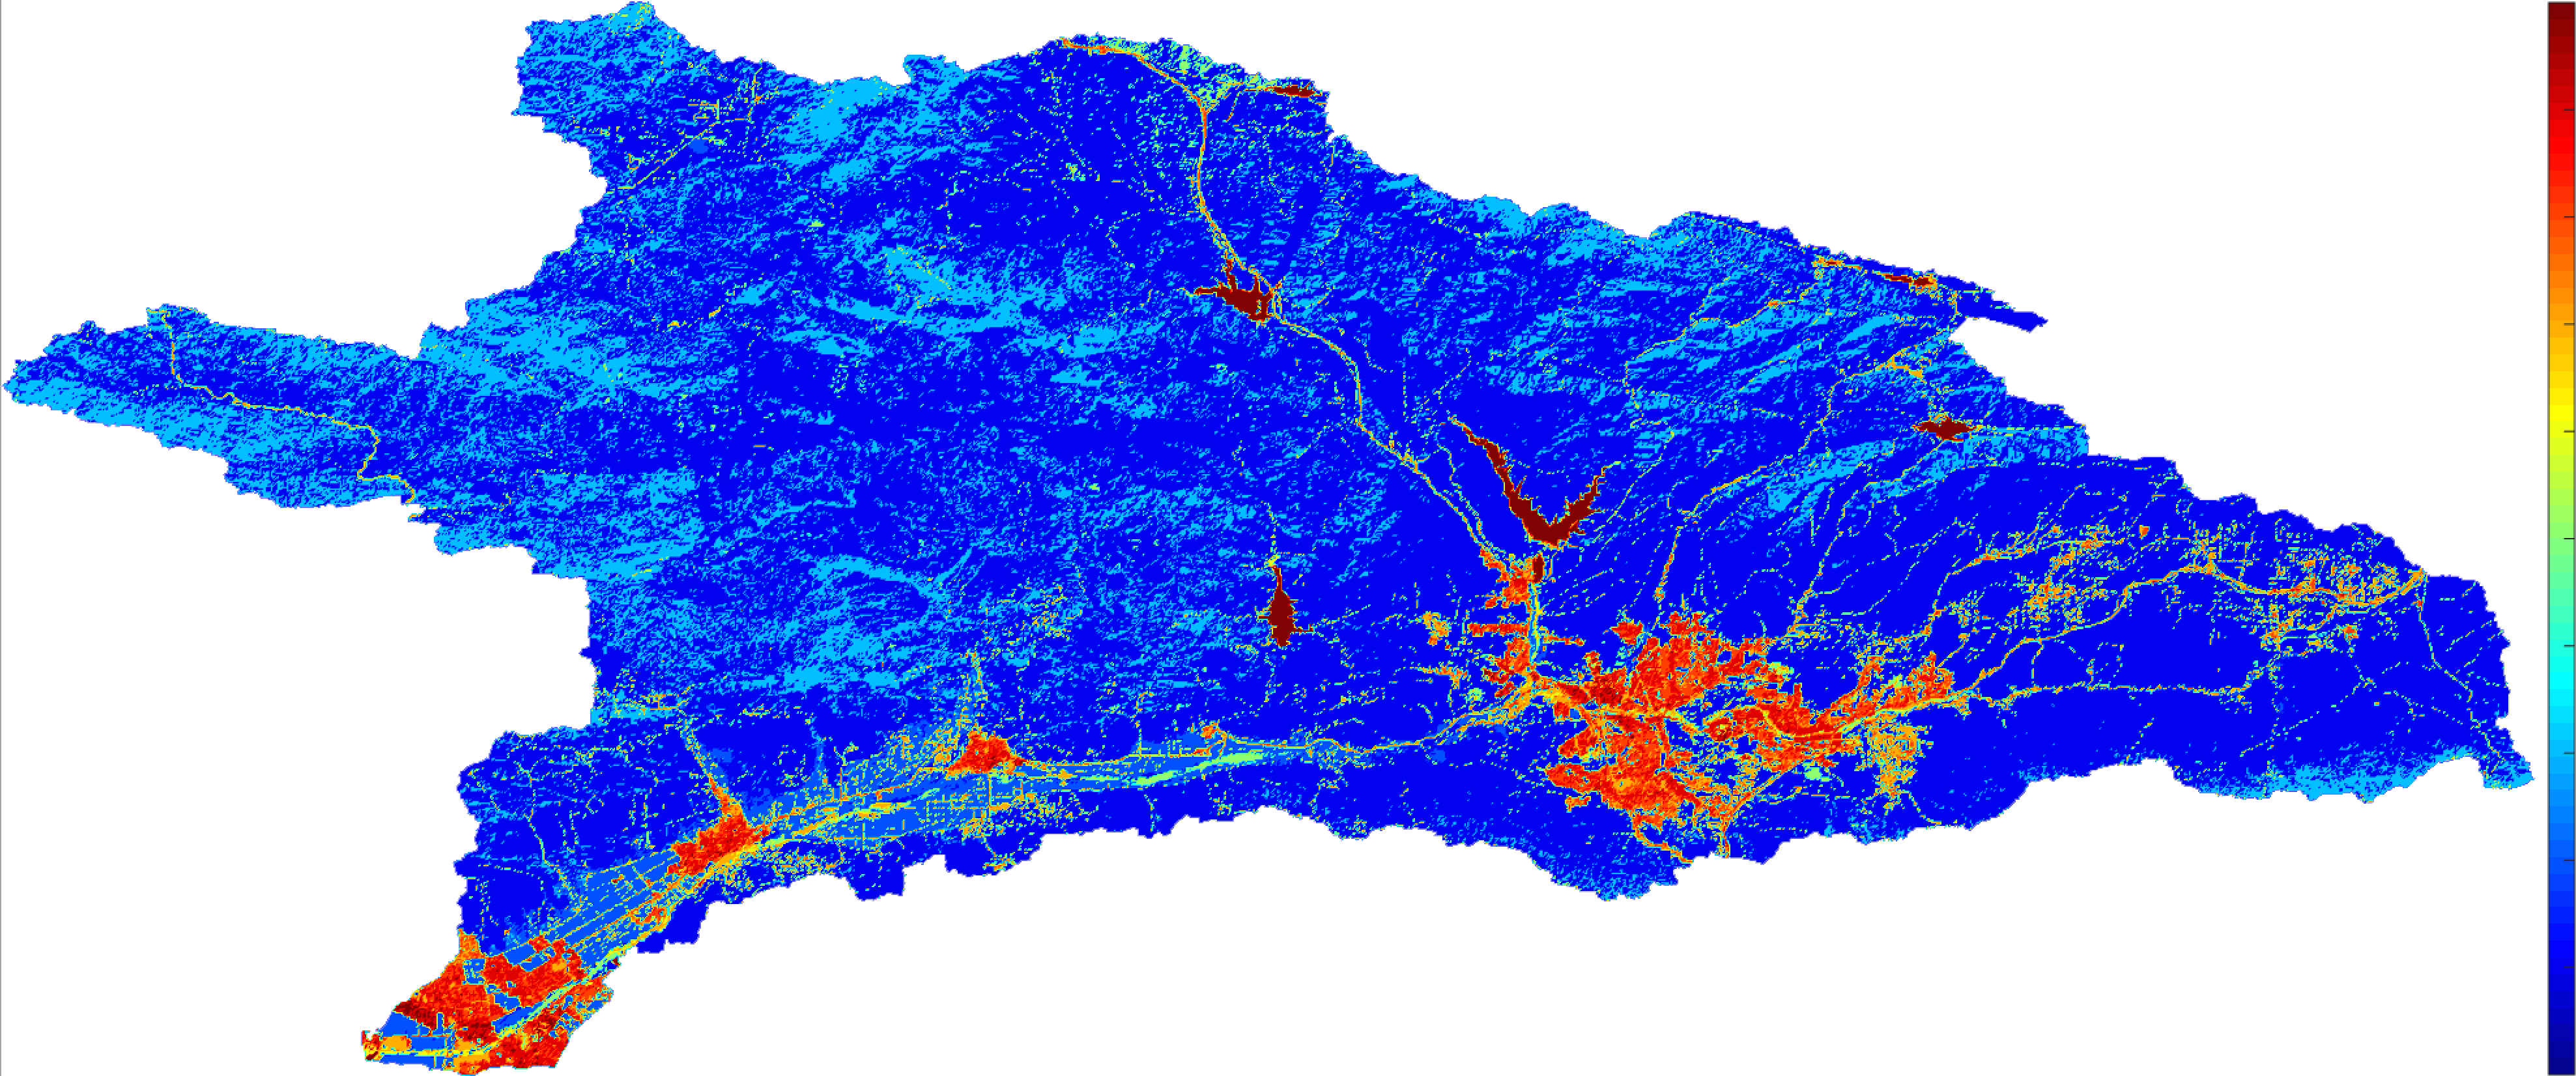
\includegraphics[width=5.5in]{figures/Oxnard_DisturbanceScore.png}   
            \caption{Oxnard Region Land Use Based Disturbance Objective Scores (Blue:Low, Red:High)}
            \label{fig:Odisturbance}
            \end{center}
        \end{figure}
        
        \begin{figure}[!h]
            \begin{center}
            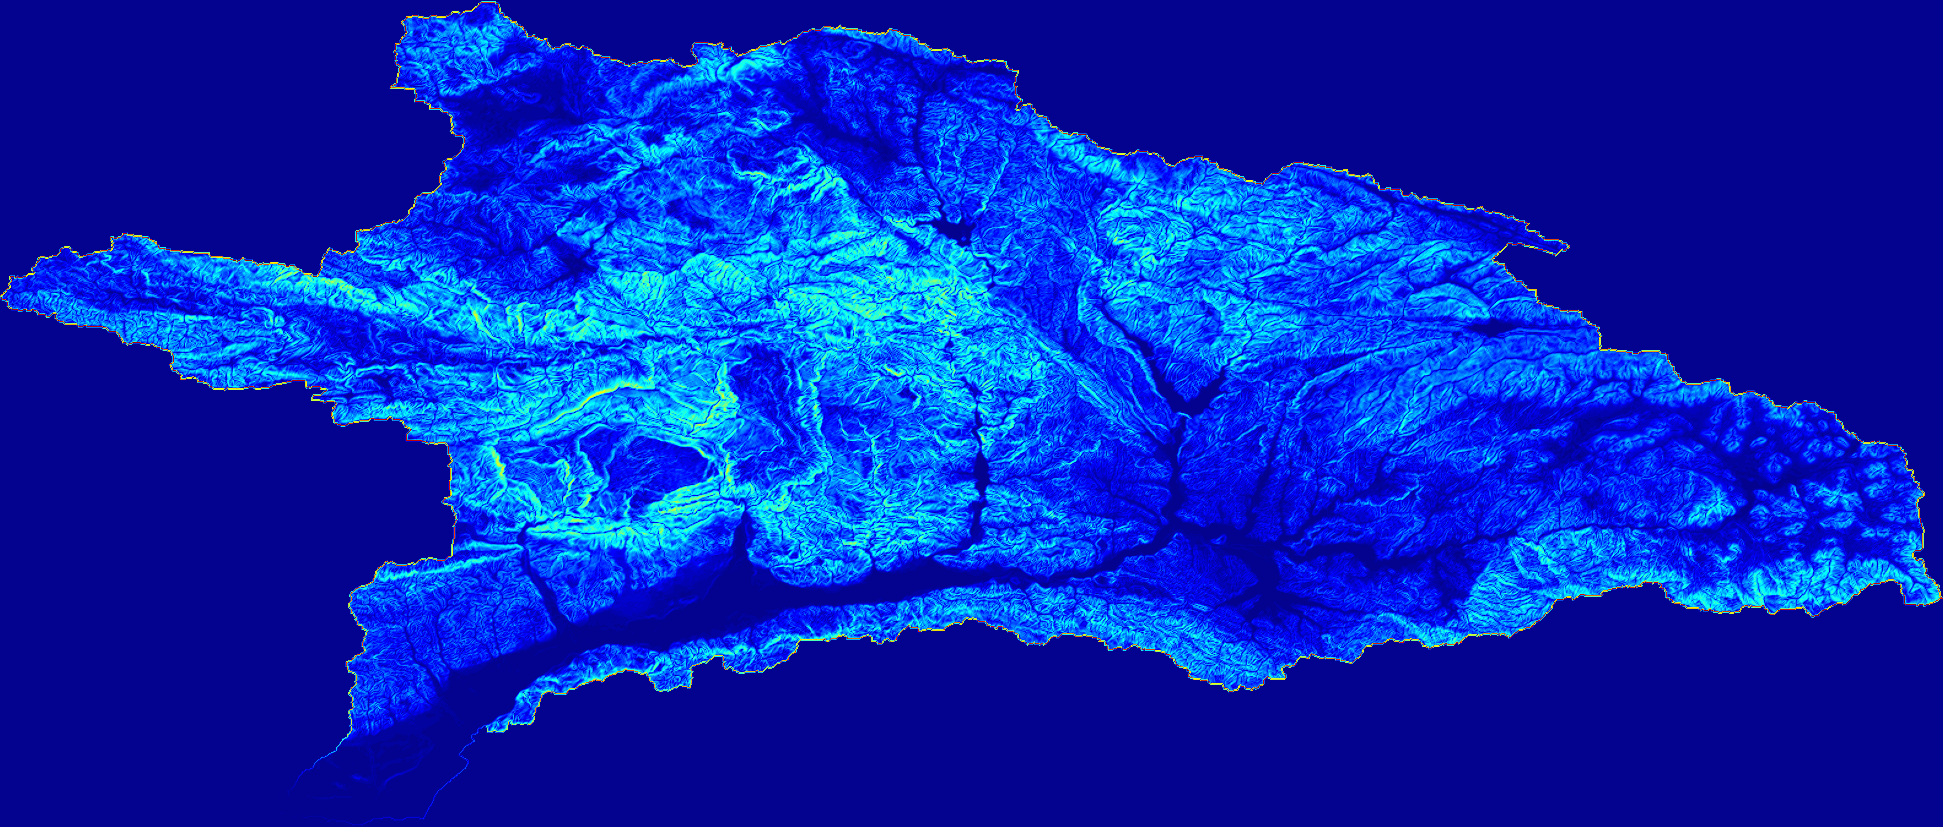
\includegraphics[width=5.5in]{figures/Oxnard_SlopeScore.png}   
            \caption{Oxnard Region Slope Based Objective Scores (Blue:Low, Red:High)}
            \label{fig:Oslope}
            \end{center}
        \end{figure}
        
    \subsection{Proposed Corridor Solutions}
    
        \begin{figure}[!h]
            \begin{center}
            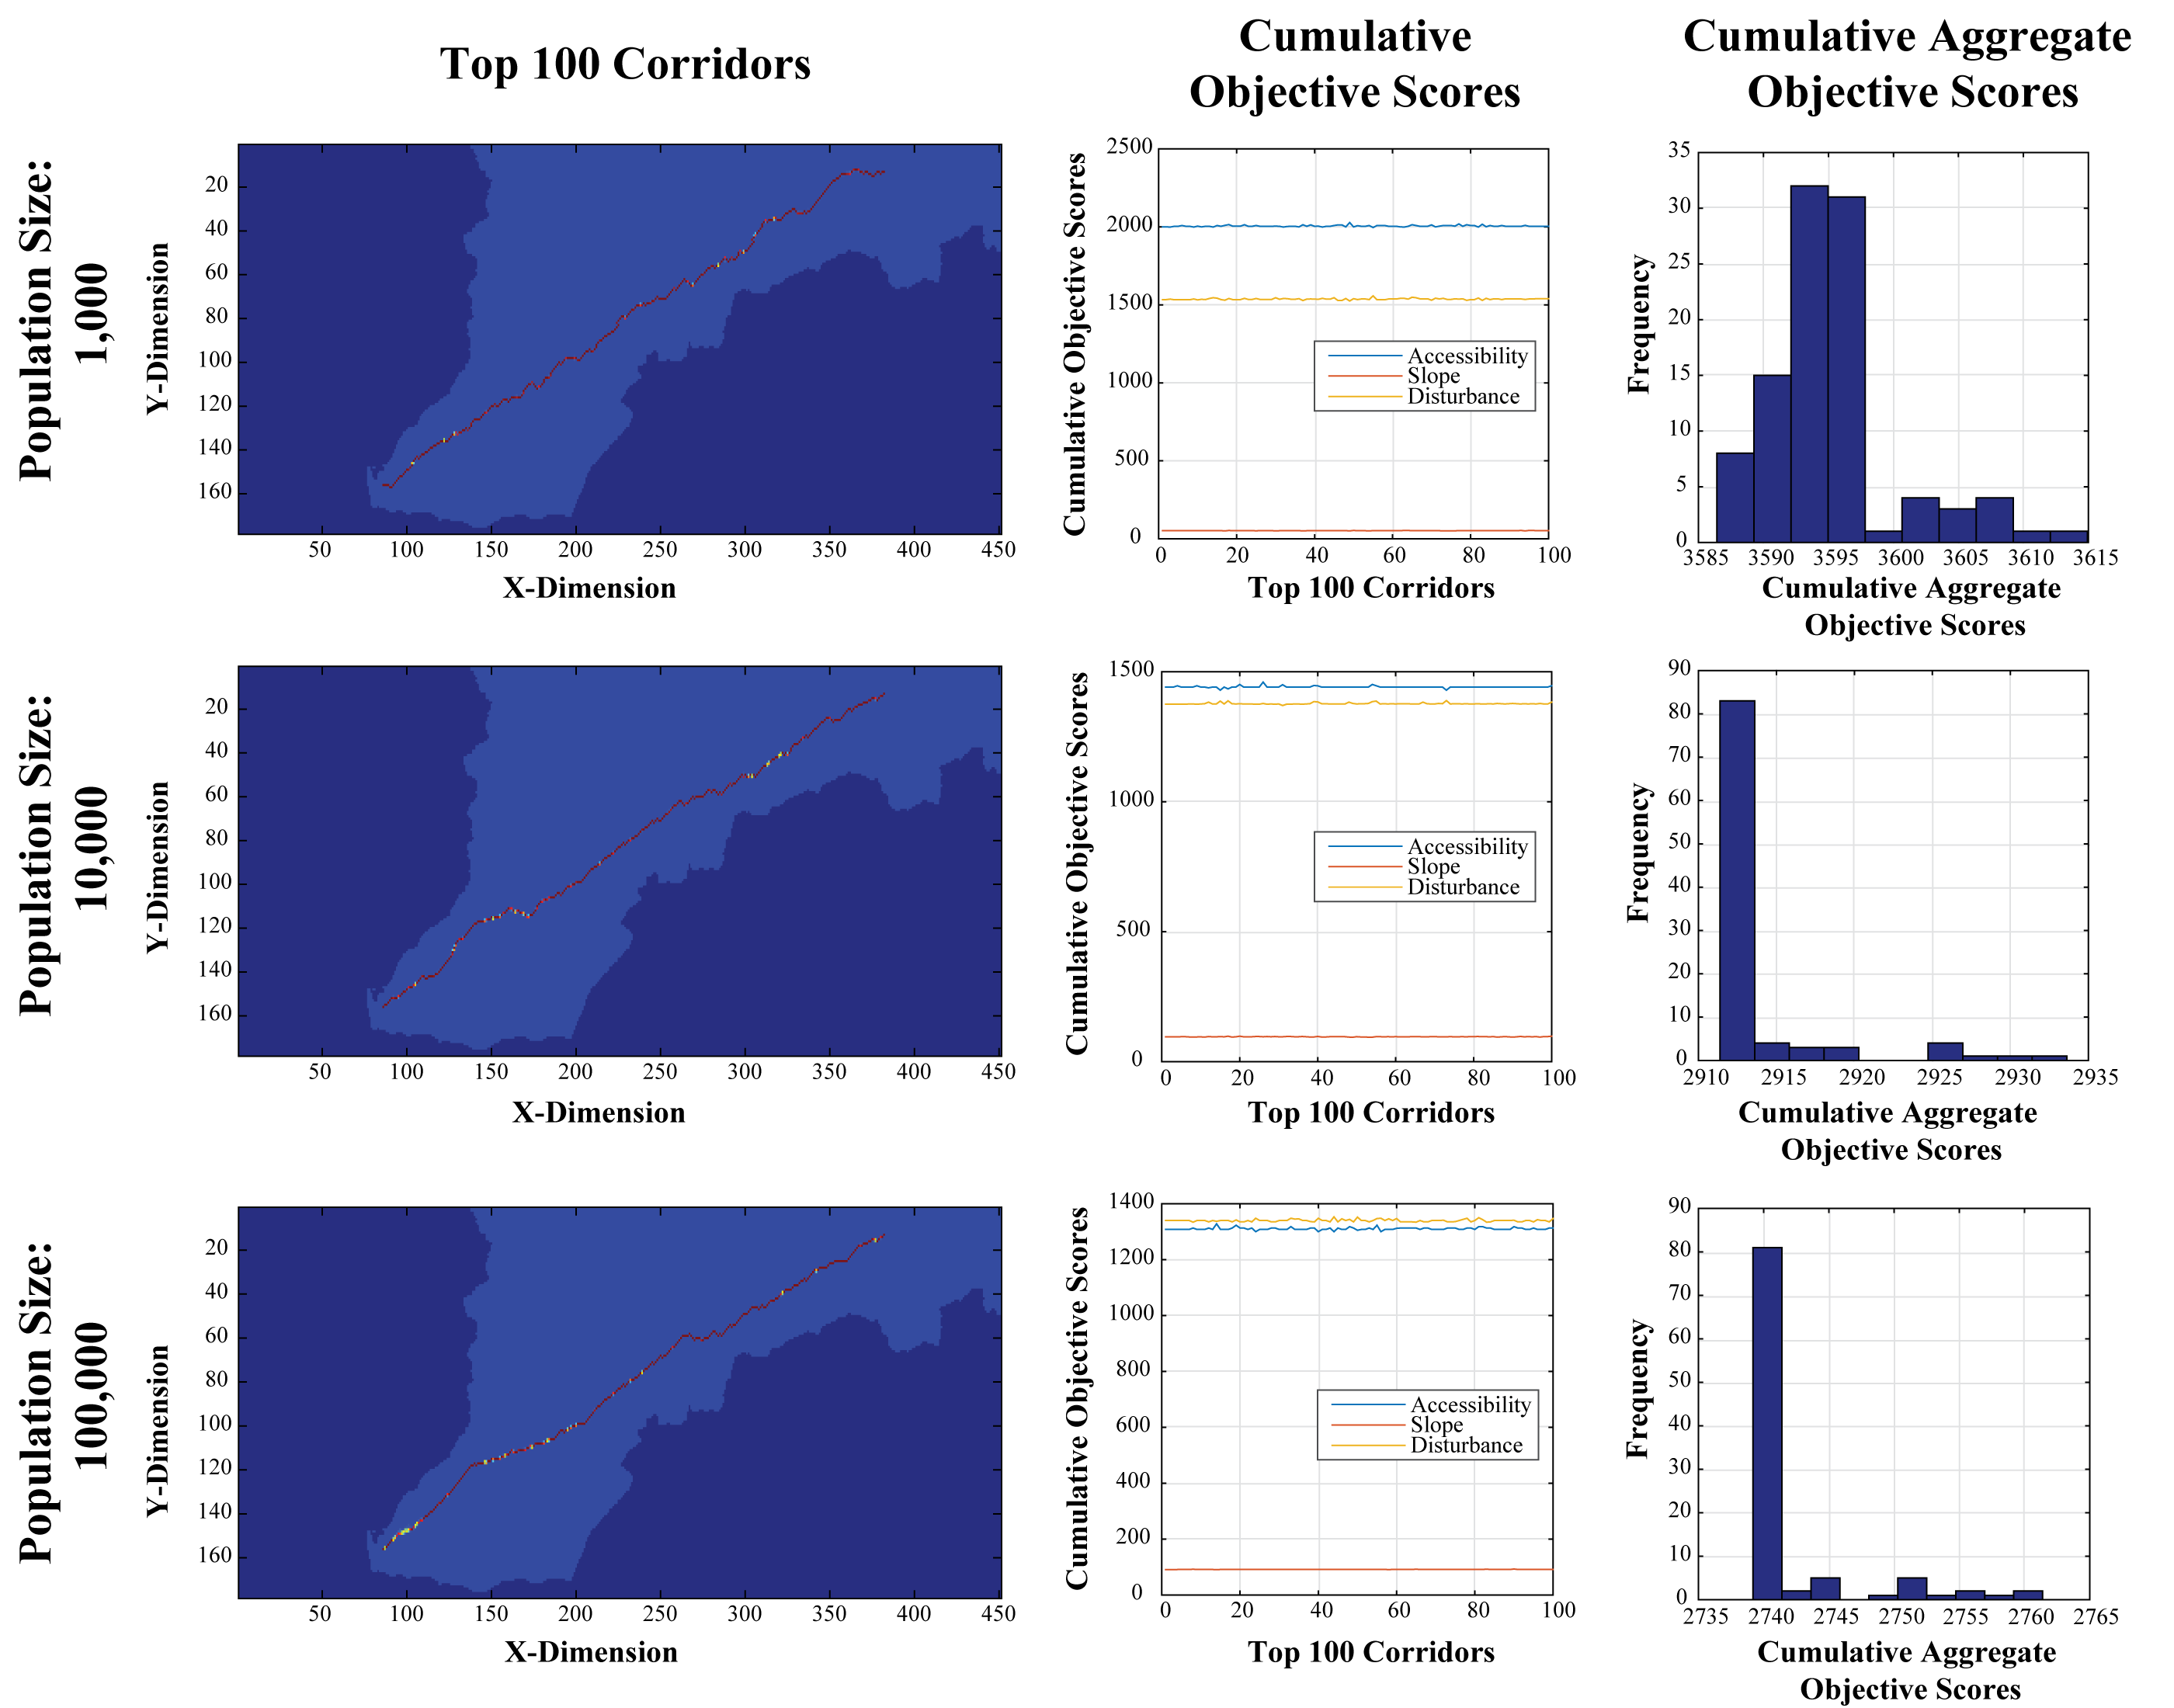
\includegraphics[width=6in]{figures/Oxnard_PathwayResults.png}   
            \caption{Oxnard Region Corridor Analysis Results}
            \label{fig:Oresults}
            \end{center}
        \end{figure}

        \begin{figure}[!h]
            \begin{center}
            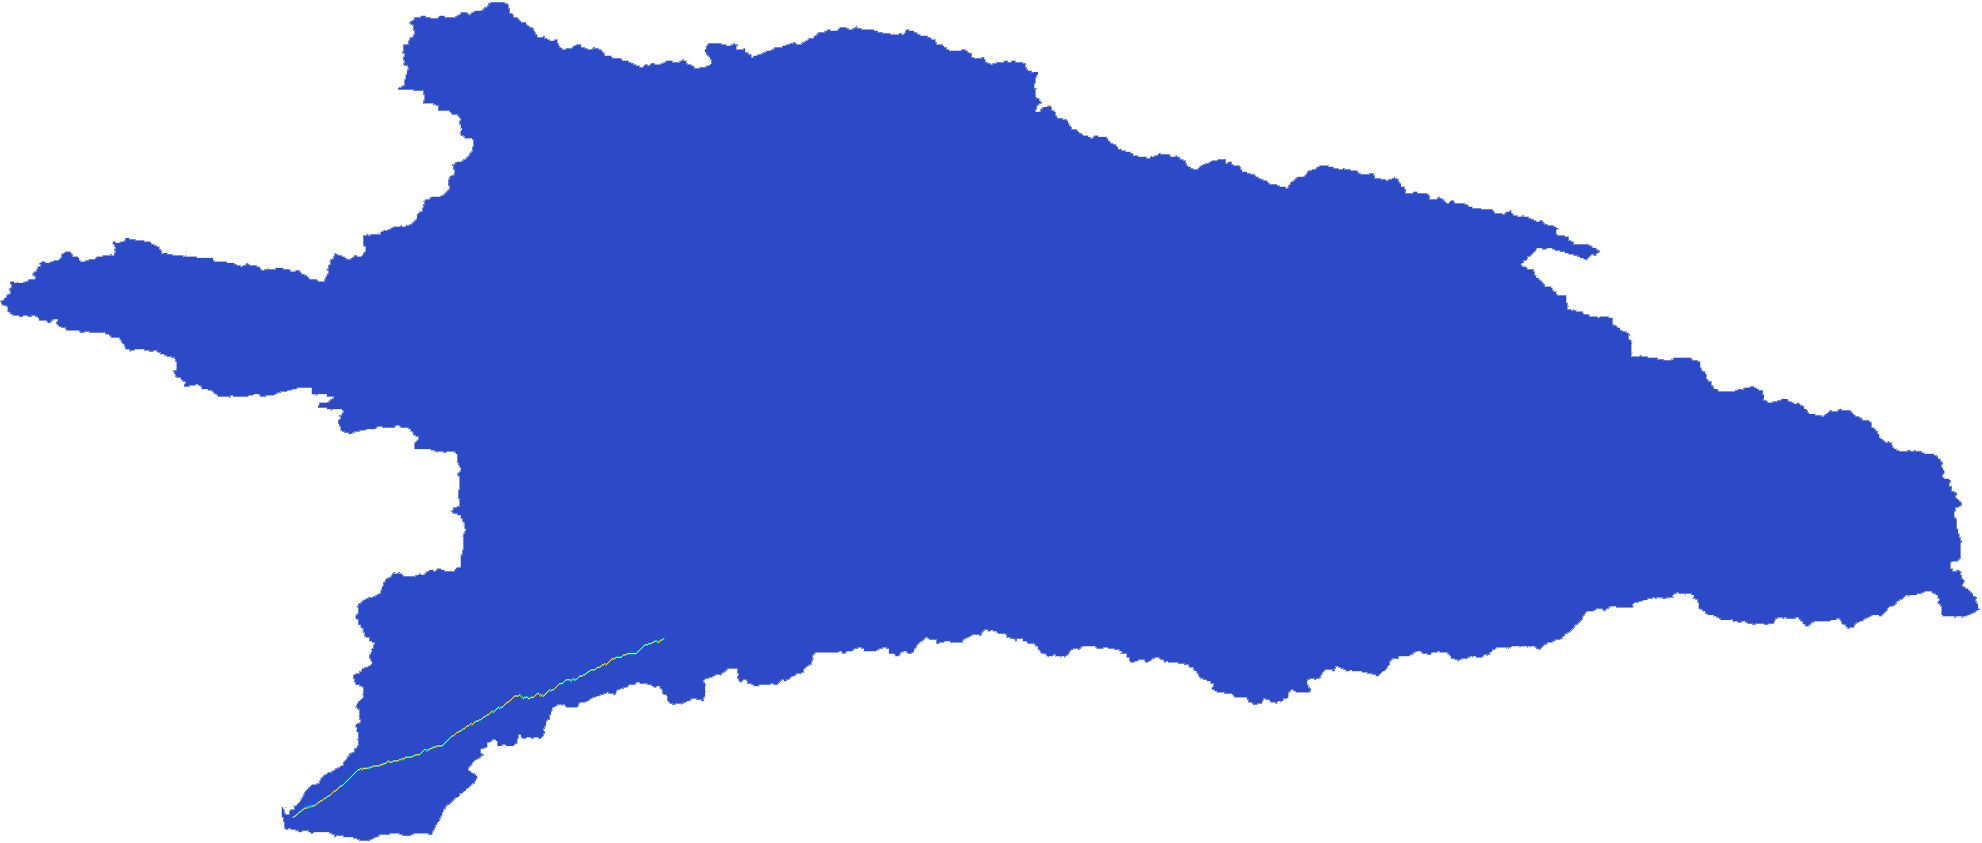
\includegraphics[width=5.5in]{figures/Oxnard_PathwayLarge.png}   
            \caption{Oxnard Region Top 100 Corridors (Pop Size: 100,000) Basin Wide Overview}
            \label{fig:OsolutionOverview}
            \end{center}
        \end{figure}
    
    \subsection{Anticipated Distribution of Life Cycle Energy Usages and Net Water Savings}    
        
\section{San Diego Region}

    \subsection{Regional Context}
    
    \begin{itemize}
      \setlength{\itemsep}{0cm}
      \setlength{\parskip}{0cm}
        \item HUC-8 Code: $18070304$
        \item Total Area: $4,338.1$ $km^2$
        \item Maximum Elevation: $1,977$ $m$
        \item Minimum Elevation: $-0.7$ $m$
        \item Mean Slope: $9.38$ $\%$
        \item Standard Deviation of Slope: $8.77$ $\%$
        \item Dominant Soil Composition: Hydrologic Soil Group - B: $10-20\%$ clay, $50-90\%$ sand, $35\%$ rock fragments
    \end{itemize}
    
        \begin{figure}[!h]
            \begin{center}
            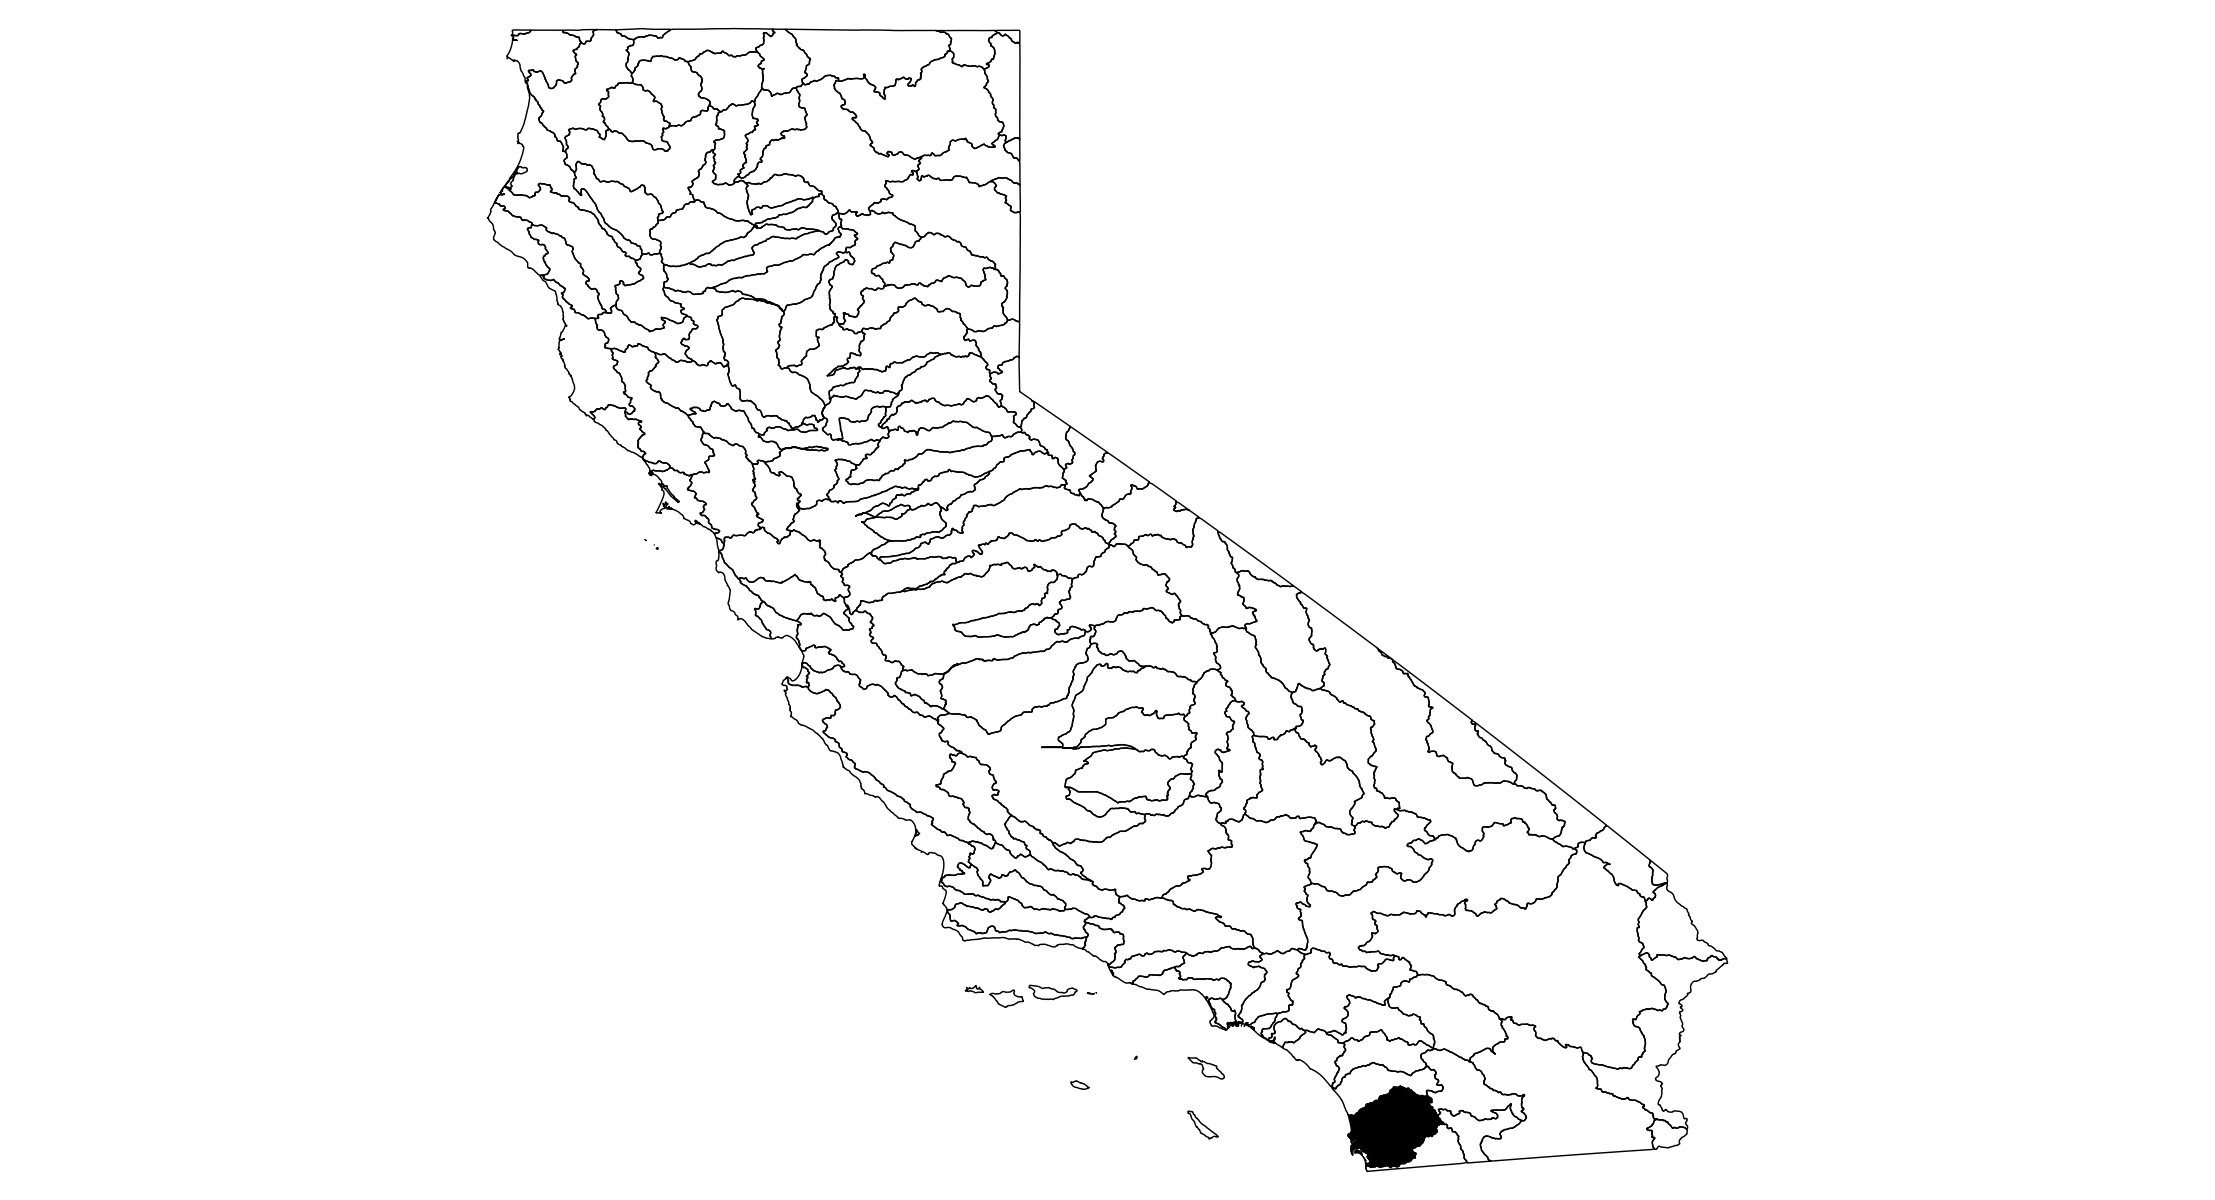
\includegraphics[width=5.5in]{figures/SanDiego_Overview.png}   
            \caption{San Diego Region Overview (Filled in Black)}
            \label{fig:SDoverview}
            \end{center}
        \end{figure}

    \subsection{Search Domain}
    
    \begin{itemize}
      \setlength{\itemsep}{0cm}
      \setlength{\parskip}{0cm}
        \item Grid Dimensions: $798$ $cells$ x $898$ $cells$
        \item Grid Cell Resolution: $100$ $m$ x $100$ $m$ ($1$ $ha$)
        \item Feasible Grid Cells: $433,808$ $cells$
    \end{itemize}
    
        \begin{figure}[!h]
            \begin{center}
            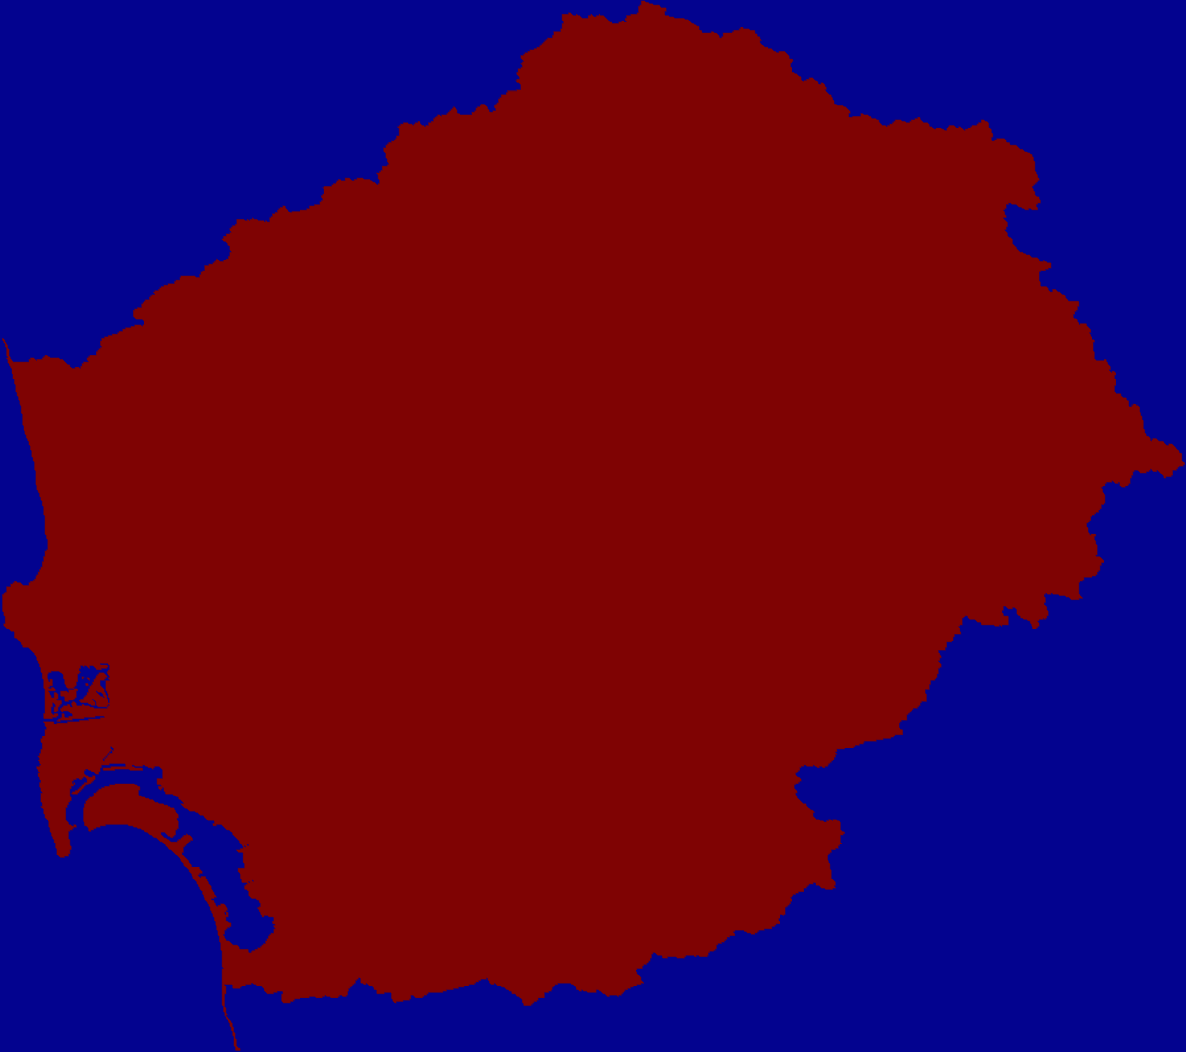
\includegraphics[width=5.5in]{figures/SanDiego_SearchDomain.png}   
            \caption{San Diego Region Search Domain (Filled in Red)}
            \label{fig:SDdomain}
            \end{center}
        \end{figure}

    \subsection{Proposed Corridor Endpoints}
    
    \begin{itemize}
      \setlength{\itemsep}{0cm}
      \setlength{\parskip}{0cm}
        \item Start Location: $(635,42)$
        \item End Destination: $(453,363)$    
        \item Shortest Euclidean Path Distance: $36,900.64$ $m$ ($36$ $km$)
    \end{itemize}
    
        \begin{figure}[!h]
            \begin{center}
            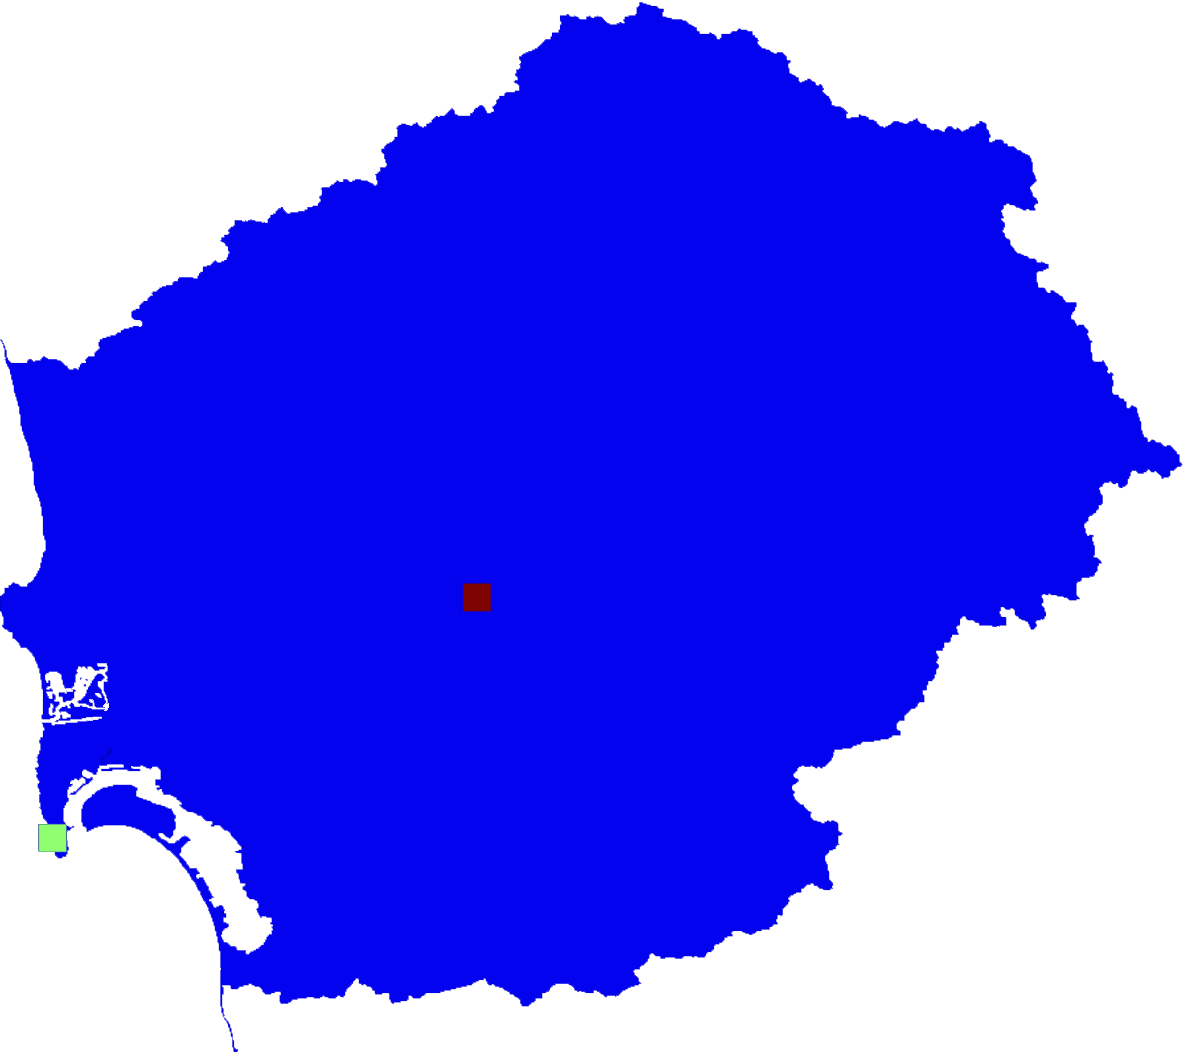
\includegraphics[width=5.5in]{figures/SanDiego_Endpoints.png}   
            \caption{San Diego Region Proposed Corridor Endpoints}
            \label{fig:SDendpoints}
            \end{center}
        \end{figure}

    \subsection{Proposed Objective Layers}

        \begin{figure}[!h]
            \begin{center}
            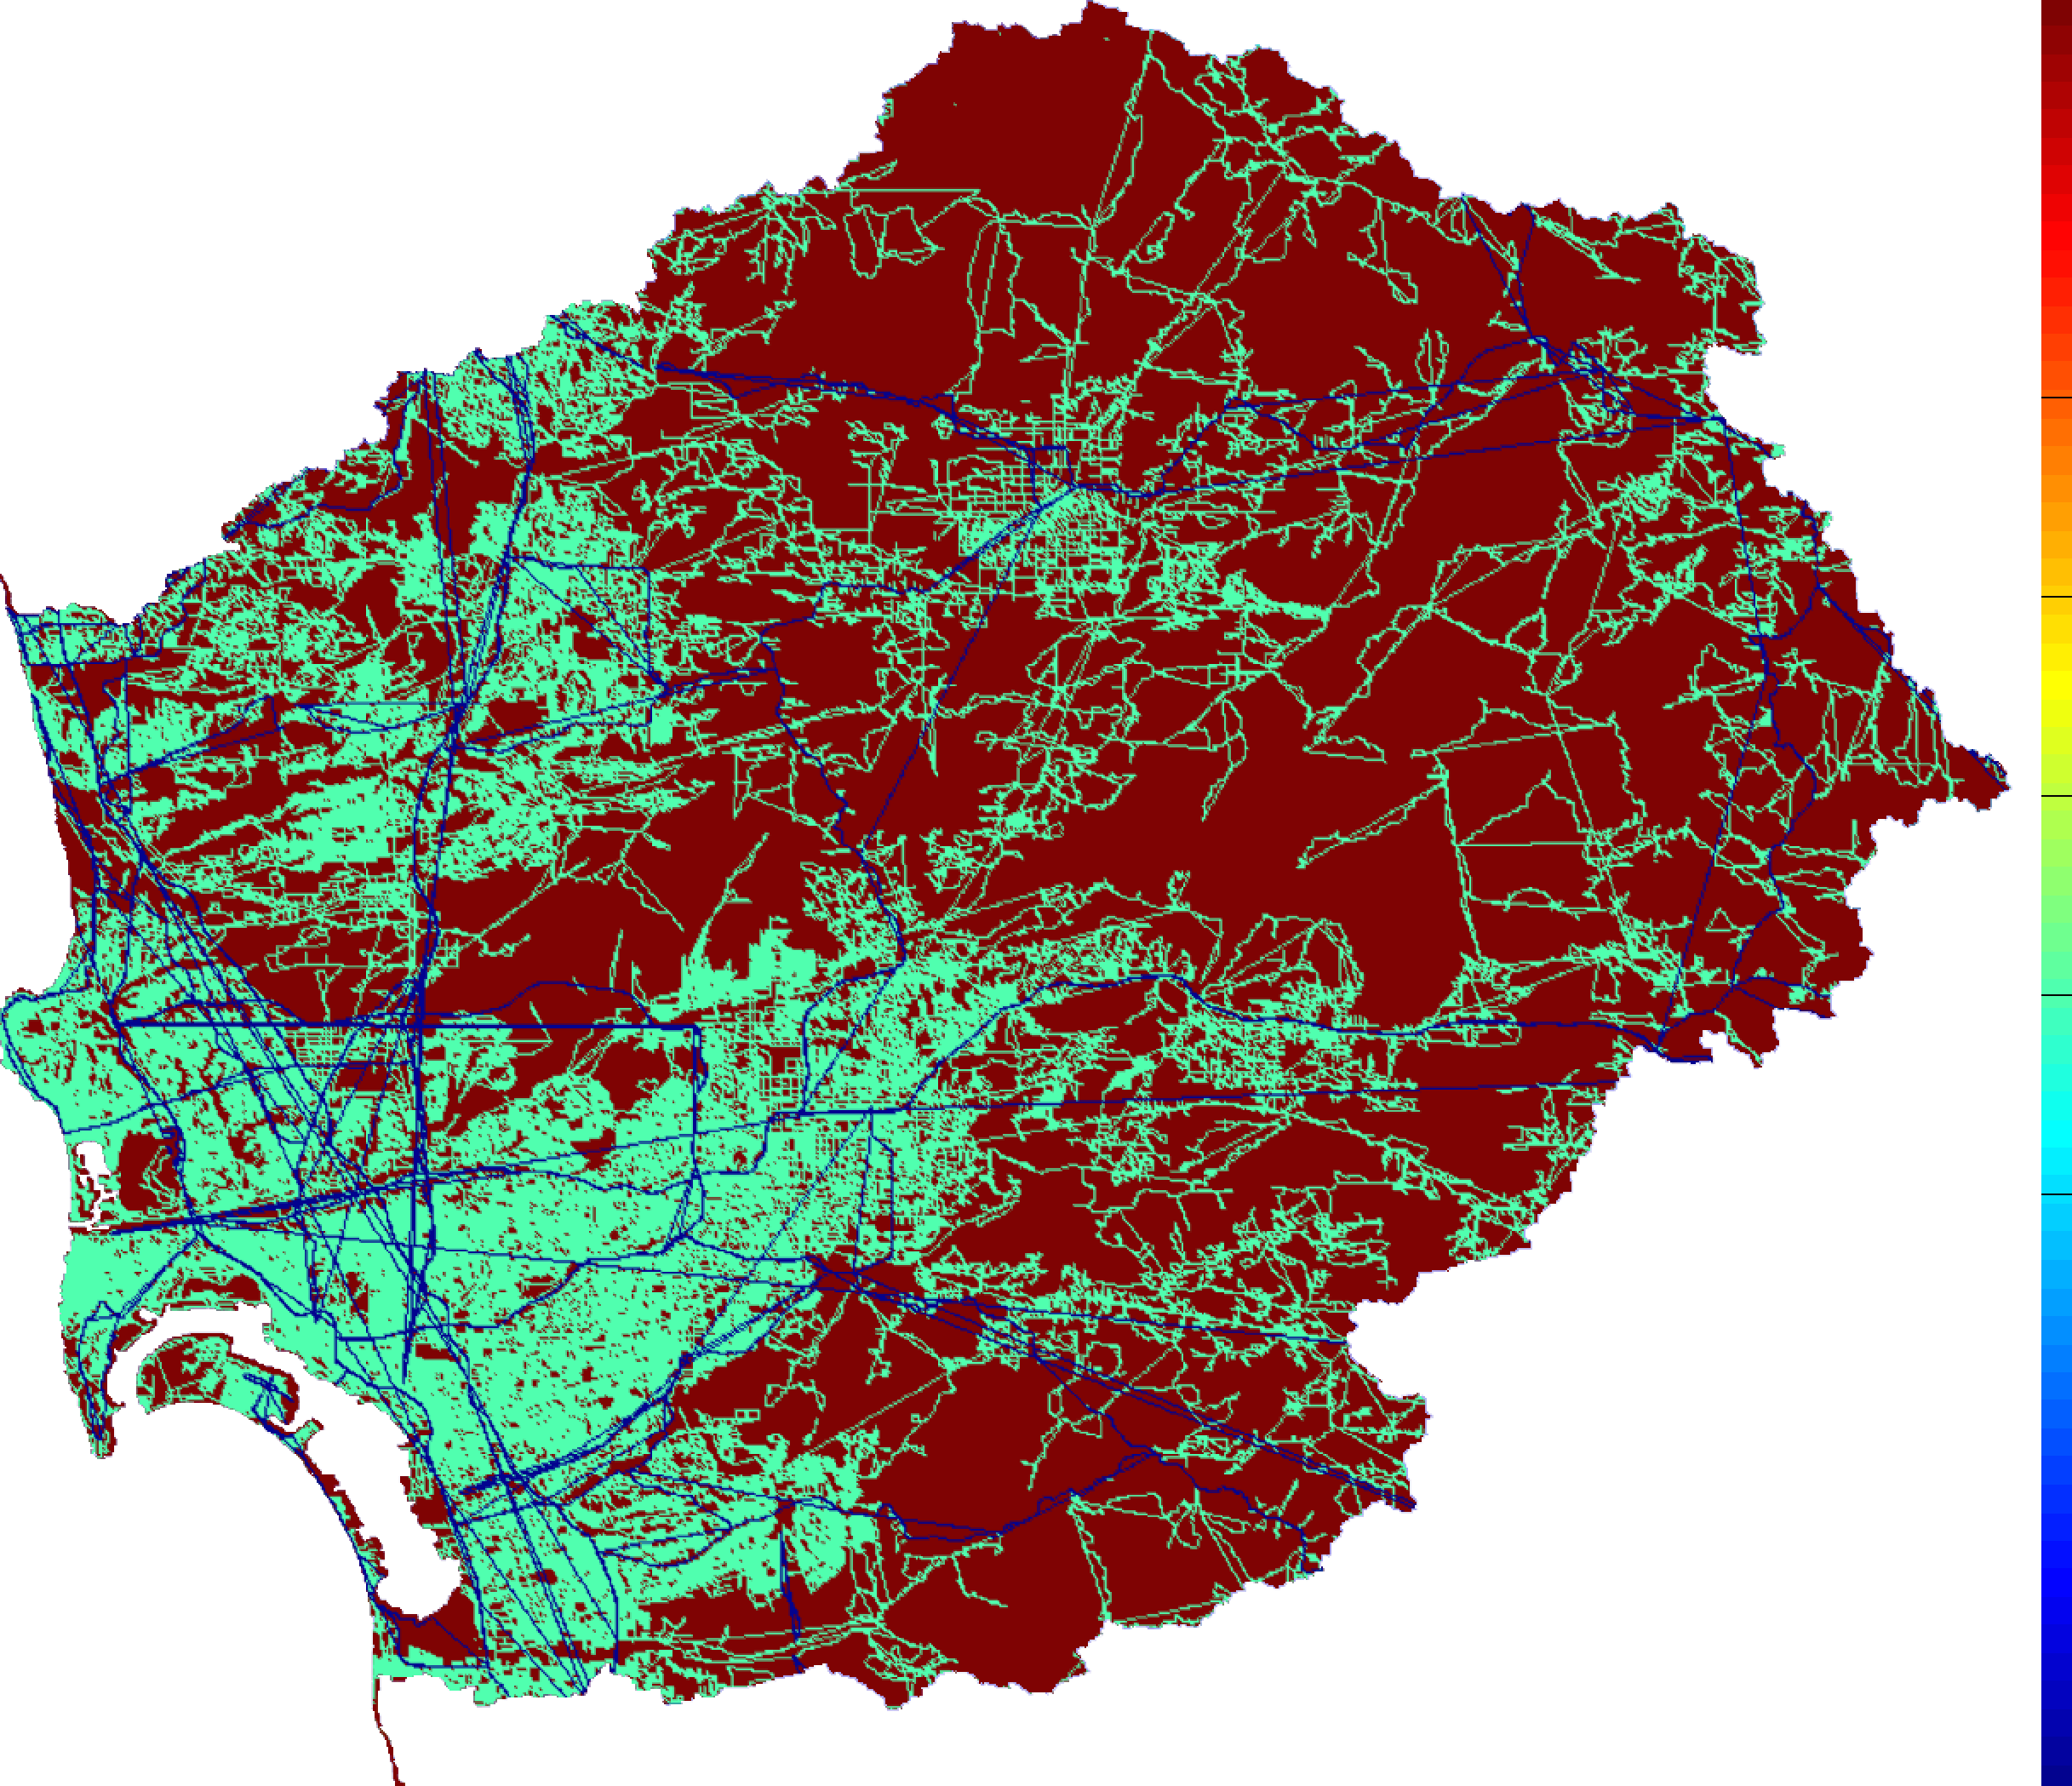
\includegraphics[width=5.5in]{figures/SanDiego_AccessibilityScore.png}   
            \caption{San Diego Region Accessibility Based Objective Scores (Blue:Low, Red:High)}
            \label{fig:SDaccessibilty}
            \end{center}
        \end{figure}

        \begin{figure}[!h]
            \begin{center}
            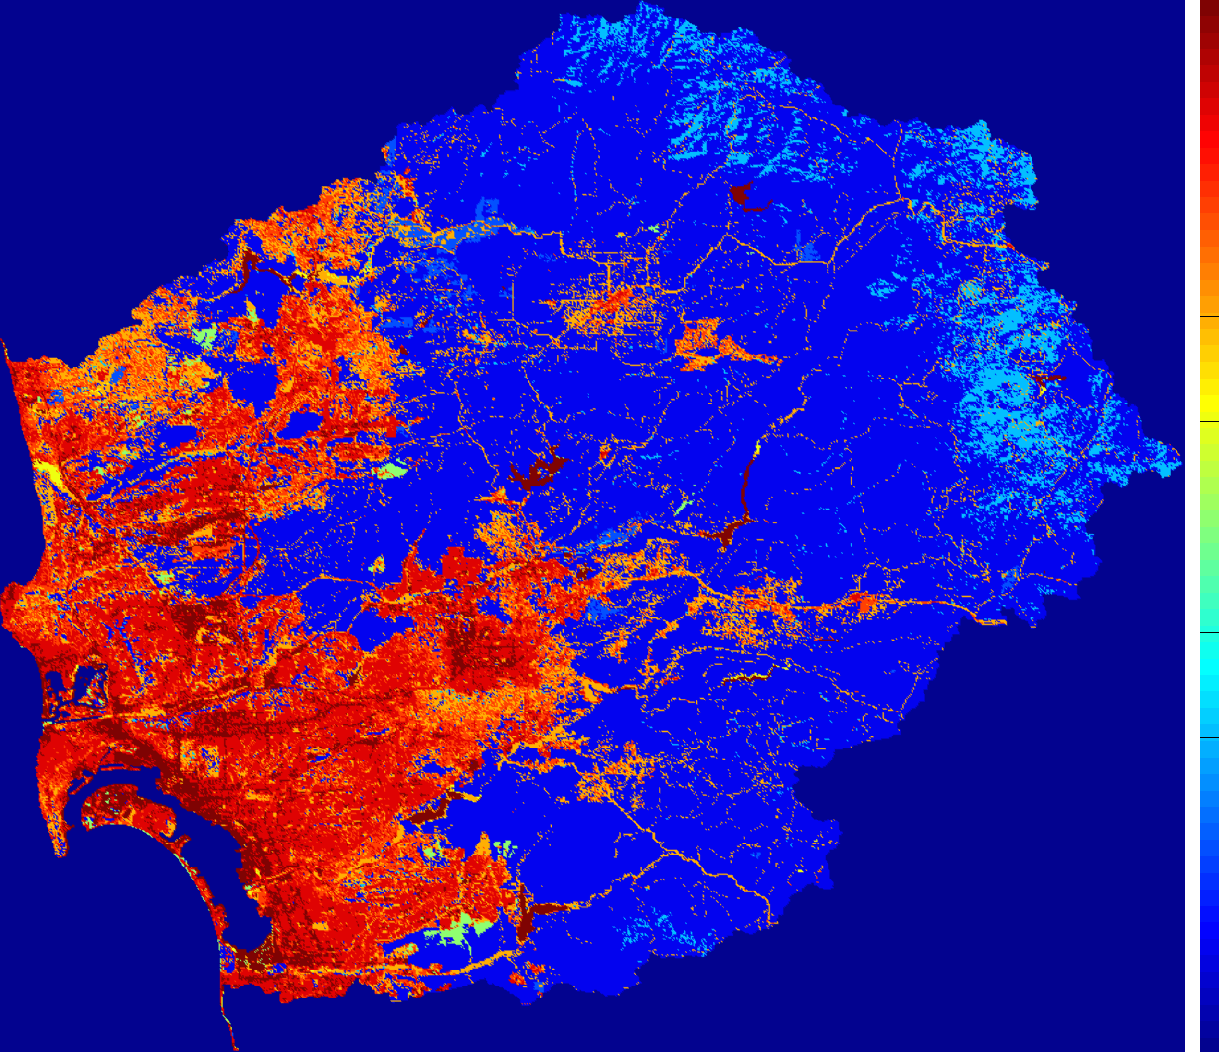
\includegraphics[width=5.5in]{figures/SanDiego_DisturbanceScore.png}   
            \caption{San Diego Region Land Use Disturbance Based Objective Scores (Blue:Low, Red:High)}
            \label{fig:SDdisturbance}
            \end{center}
        \end{figure}
        
        \begin{figure}[!h]
            \begin{center}
            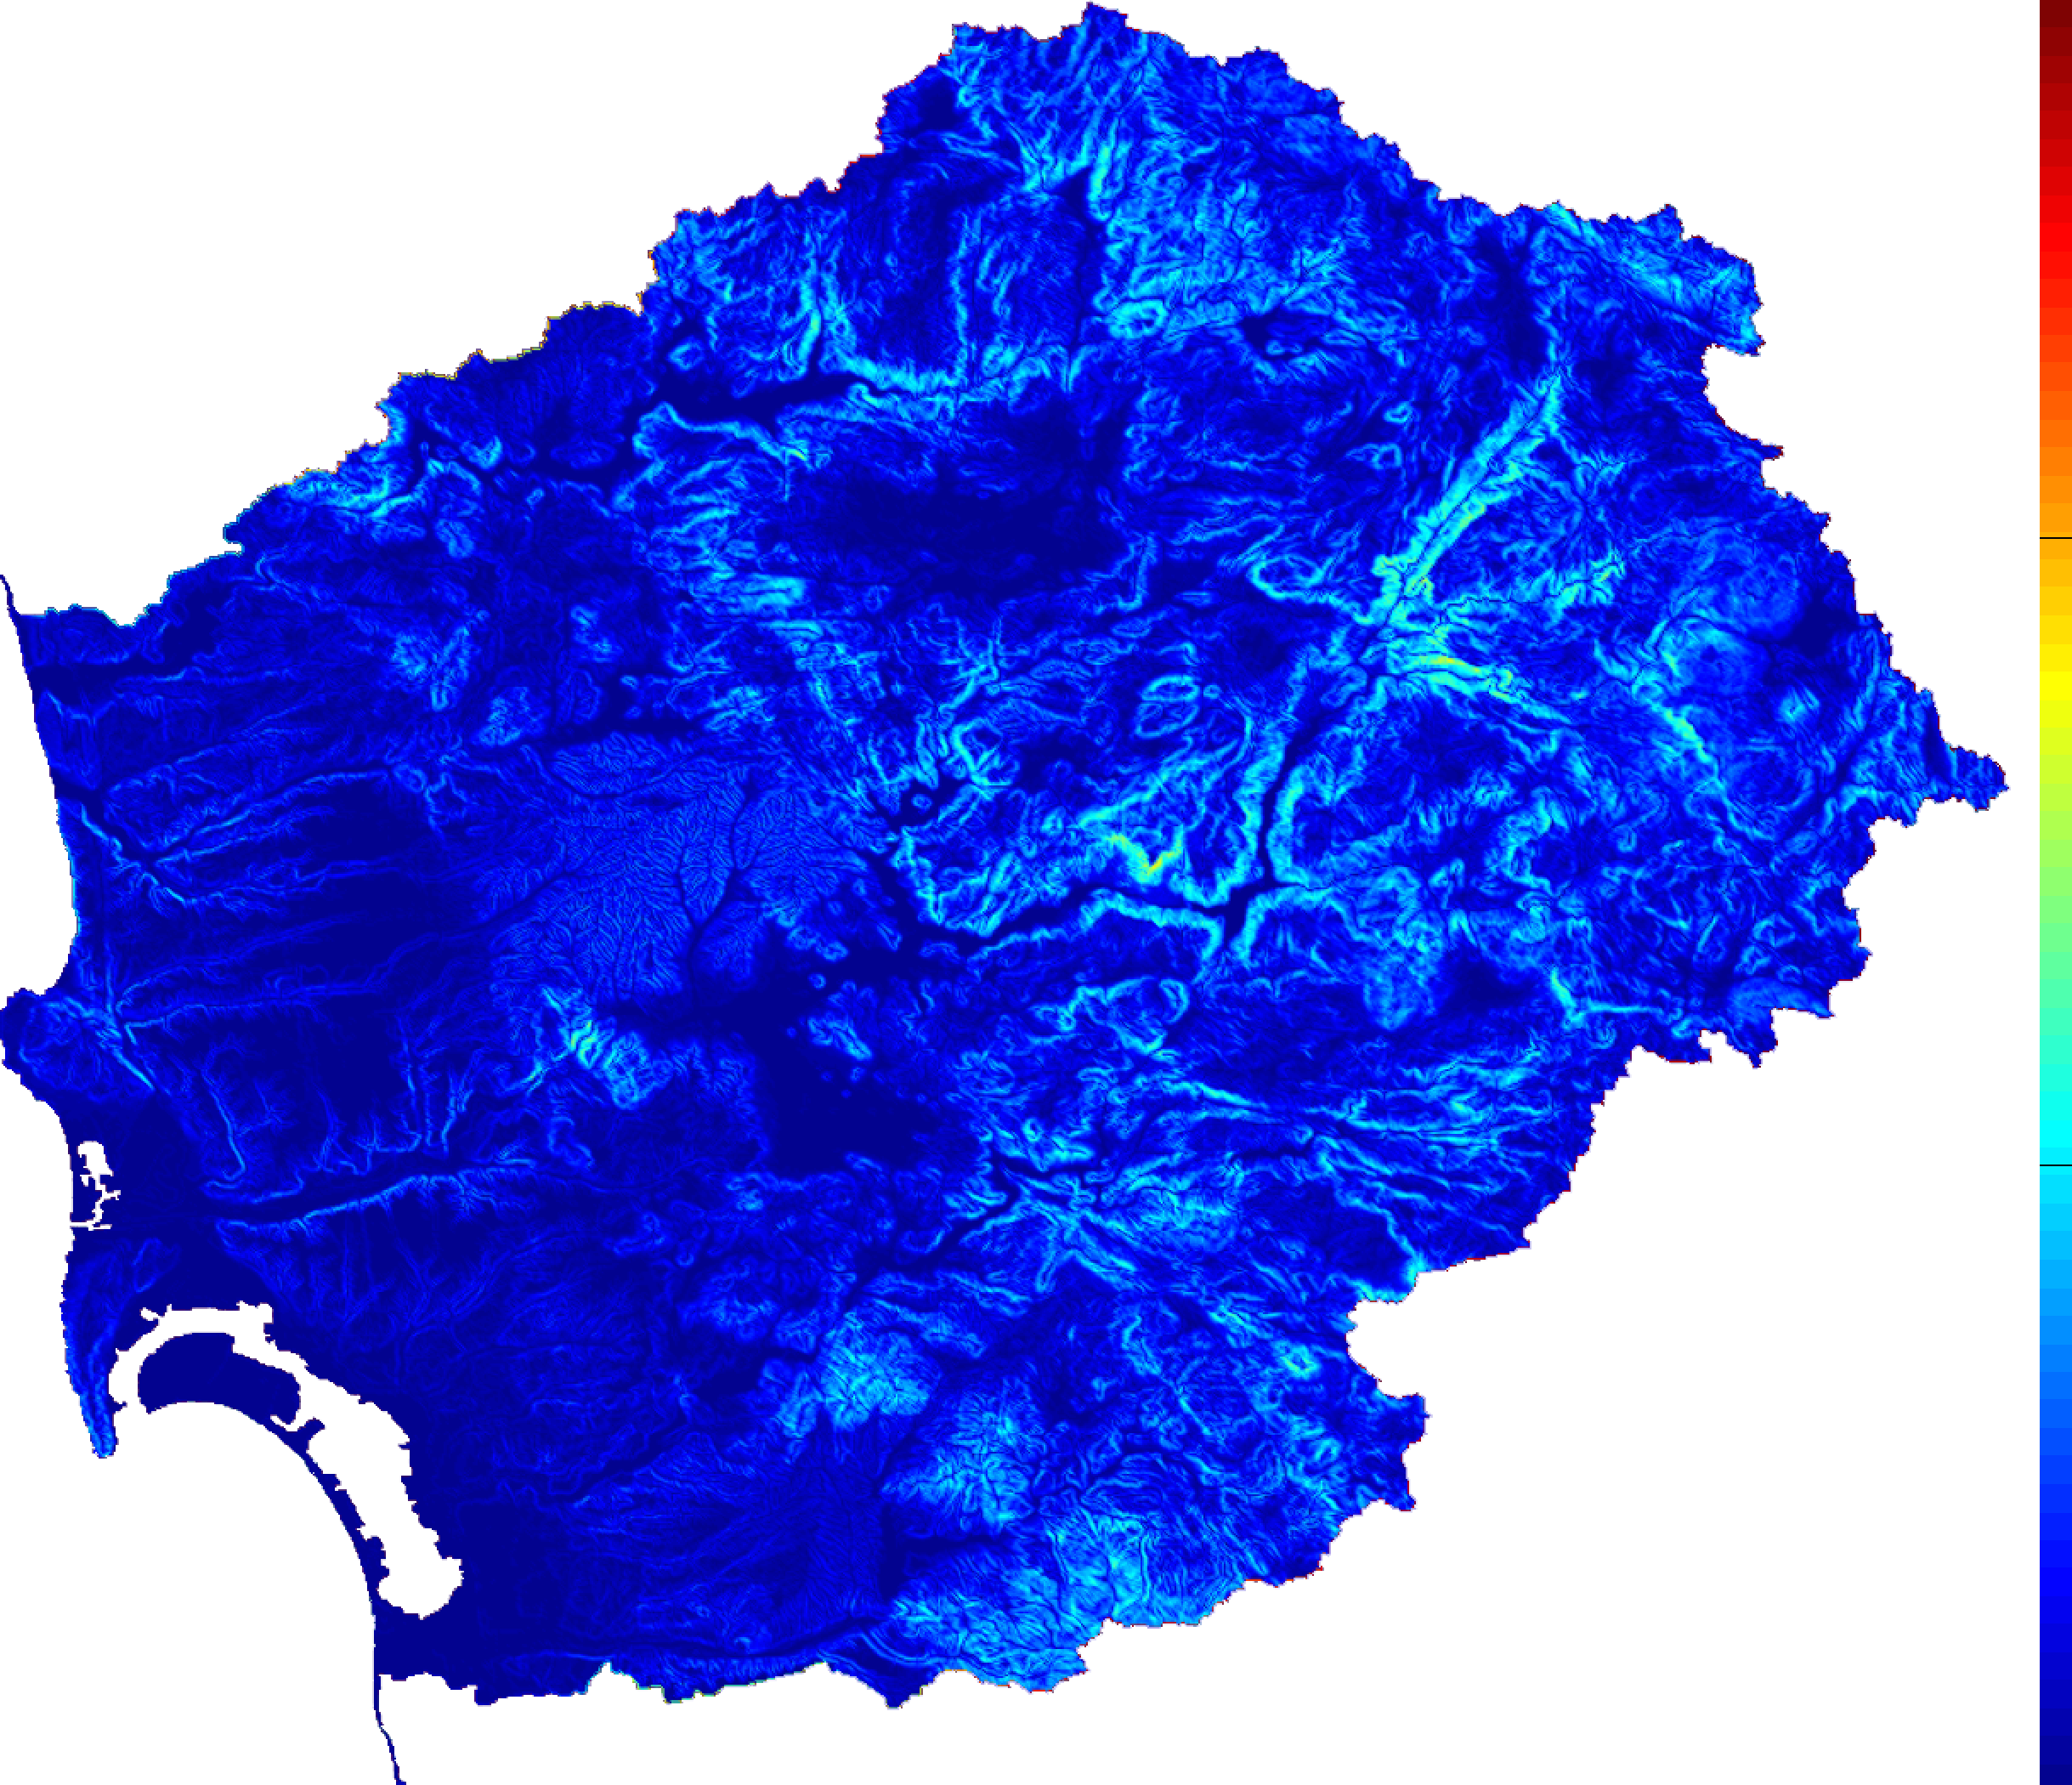
\includegraphics[width=5.5in]{figures/SanDiego_SlopeScore.png}   
            \caption{San Diego Region Slope Based Objective Scores (Blue:Low, Red:High)}
            \label{fig:SDslope}
            \end{center}
        \end{figure}
        
    \subsection{Proposed Corridor Solutions}
    
        \begin{figure}[!h]
            \begin{center}
            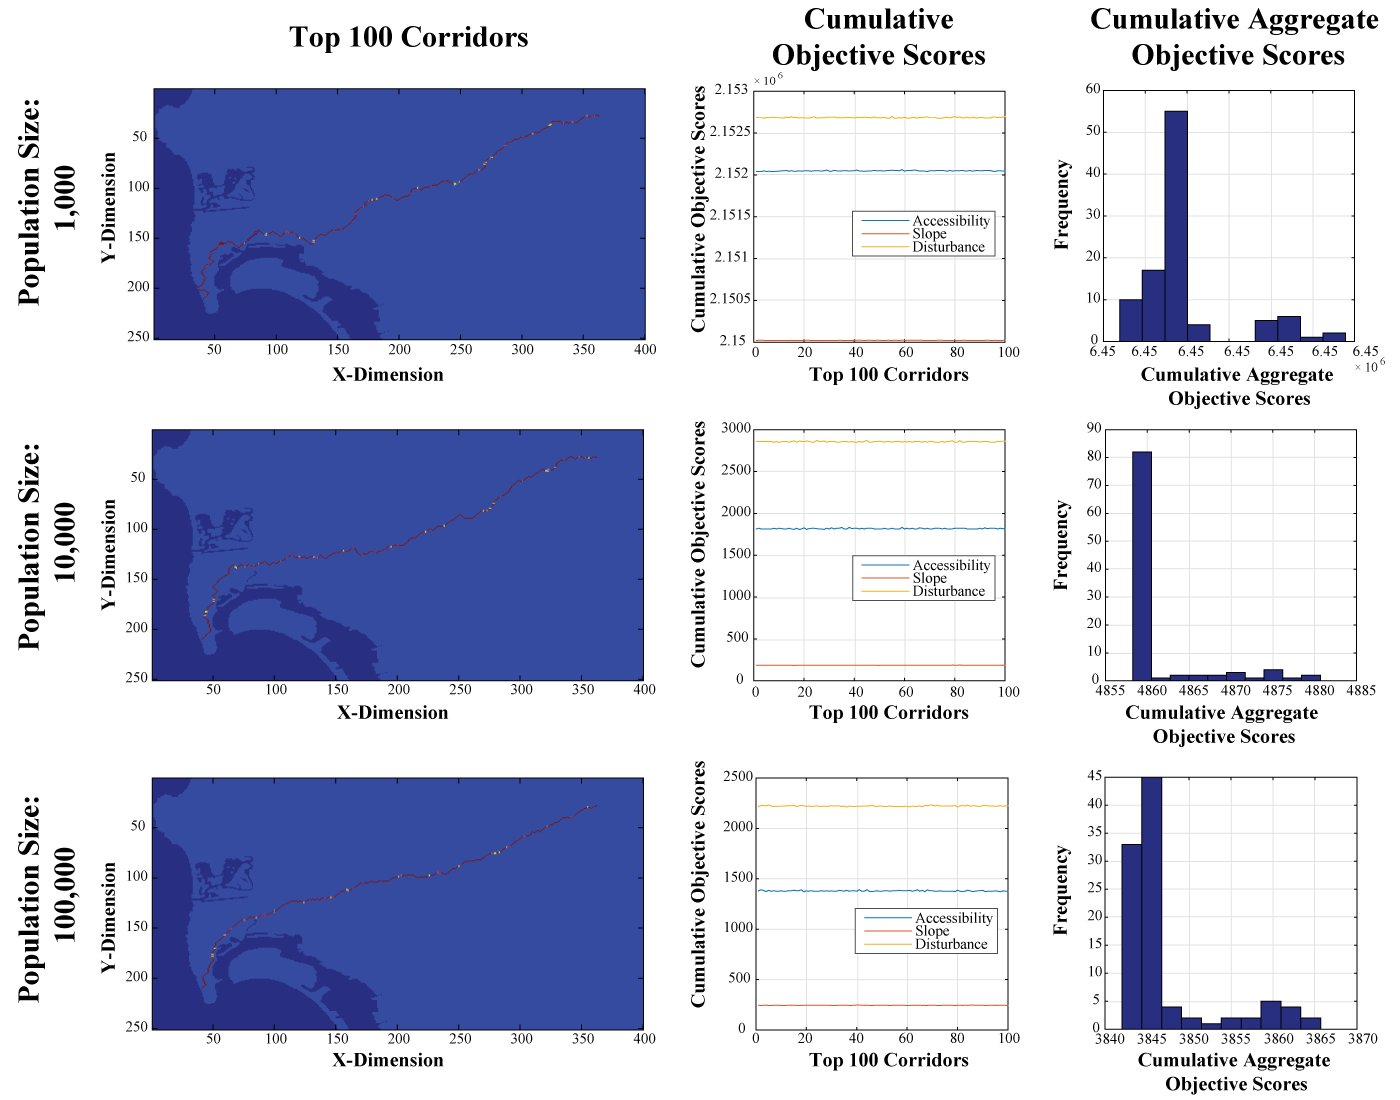
\includegraphics[width=6in]{figures/SanDiego_PathwayResults.png}   
            \caption{San Diego Region Corridor Analysis Results}
            \label{fig:SDresults}
            \end{center}
        \end{figure}

        \begin{figure}[!h]
            \begin{center}
            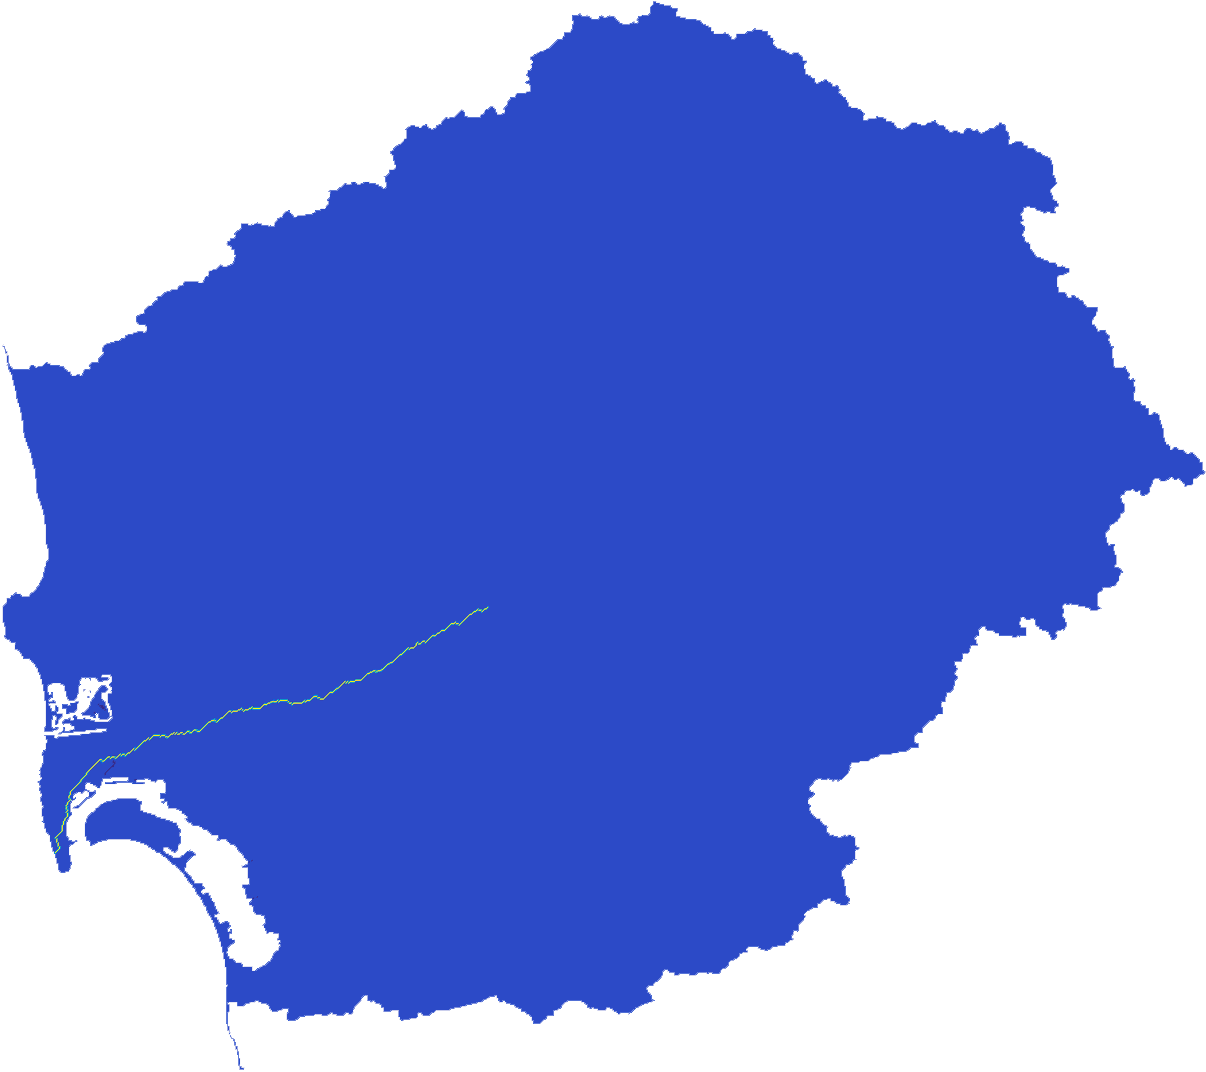
\includegraphics[width=5.5in]{figures/SanDiego_PathwayLarge.png}   
            \caption{San Diego Region Top 100 Corridors (Pop Size: 100,000) Basin Wide Overview}
            \label{fig:SDsolutionOverview}
            \end{center}
        \end{figure}
    
    \subsection{Anticipated Distribution of Life Cycle Energy Usages and Net Water Savings}

\section{Santa Ana -- San Bernadino Region}

    \subsection{Regional Context}

    \begin{itemize}
      \setlength{\itemsep}{0cm}
      \setlength{\parskip}{0cm}
        \item HUC-8 Code: $18070203$
        \item Total Area: $5,375.9$ $km^2$
        \item Maximum Elevation: $3,461.3$ $m$
        \item Minimum Elevation: $-0.7$ $m$
        \item Mean Slope: $10.56$ $\%$
        \item Standard Deviation of Slope: $12.21$ $\%$
        \item Dominant Soil Composition: Hydrologic Soil Group - B: $10-20\%$ clay, $50-90\%$ sand, $35\%$ rock fragments
    \end{itemize}
    
        \begin{figure}[!h]
            \begin{center}
            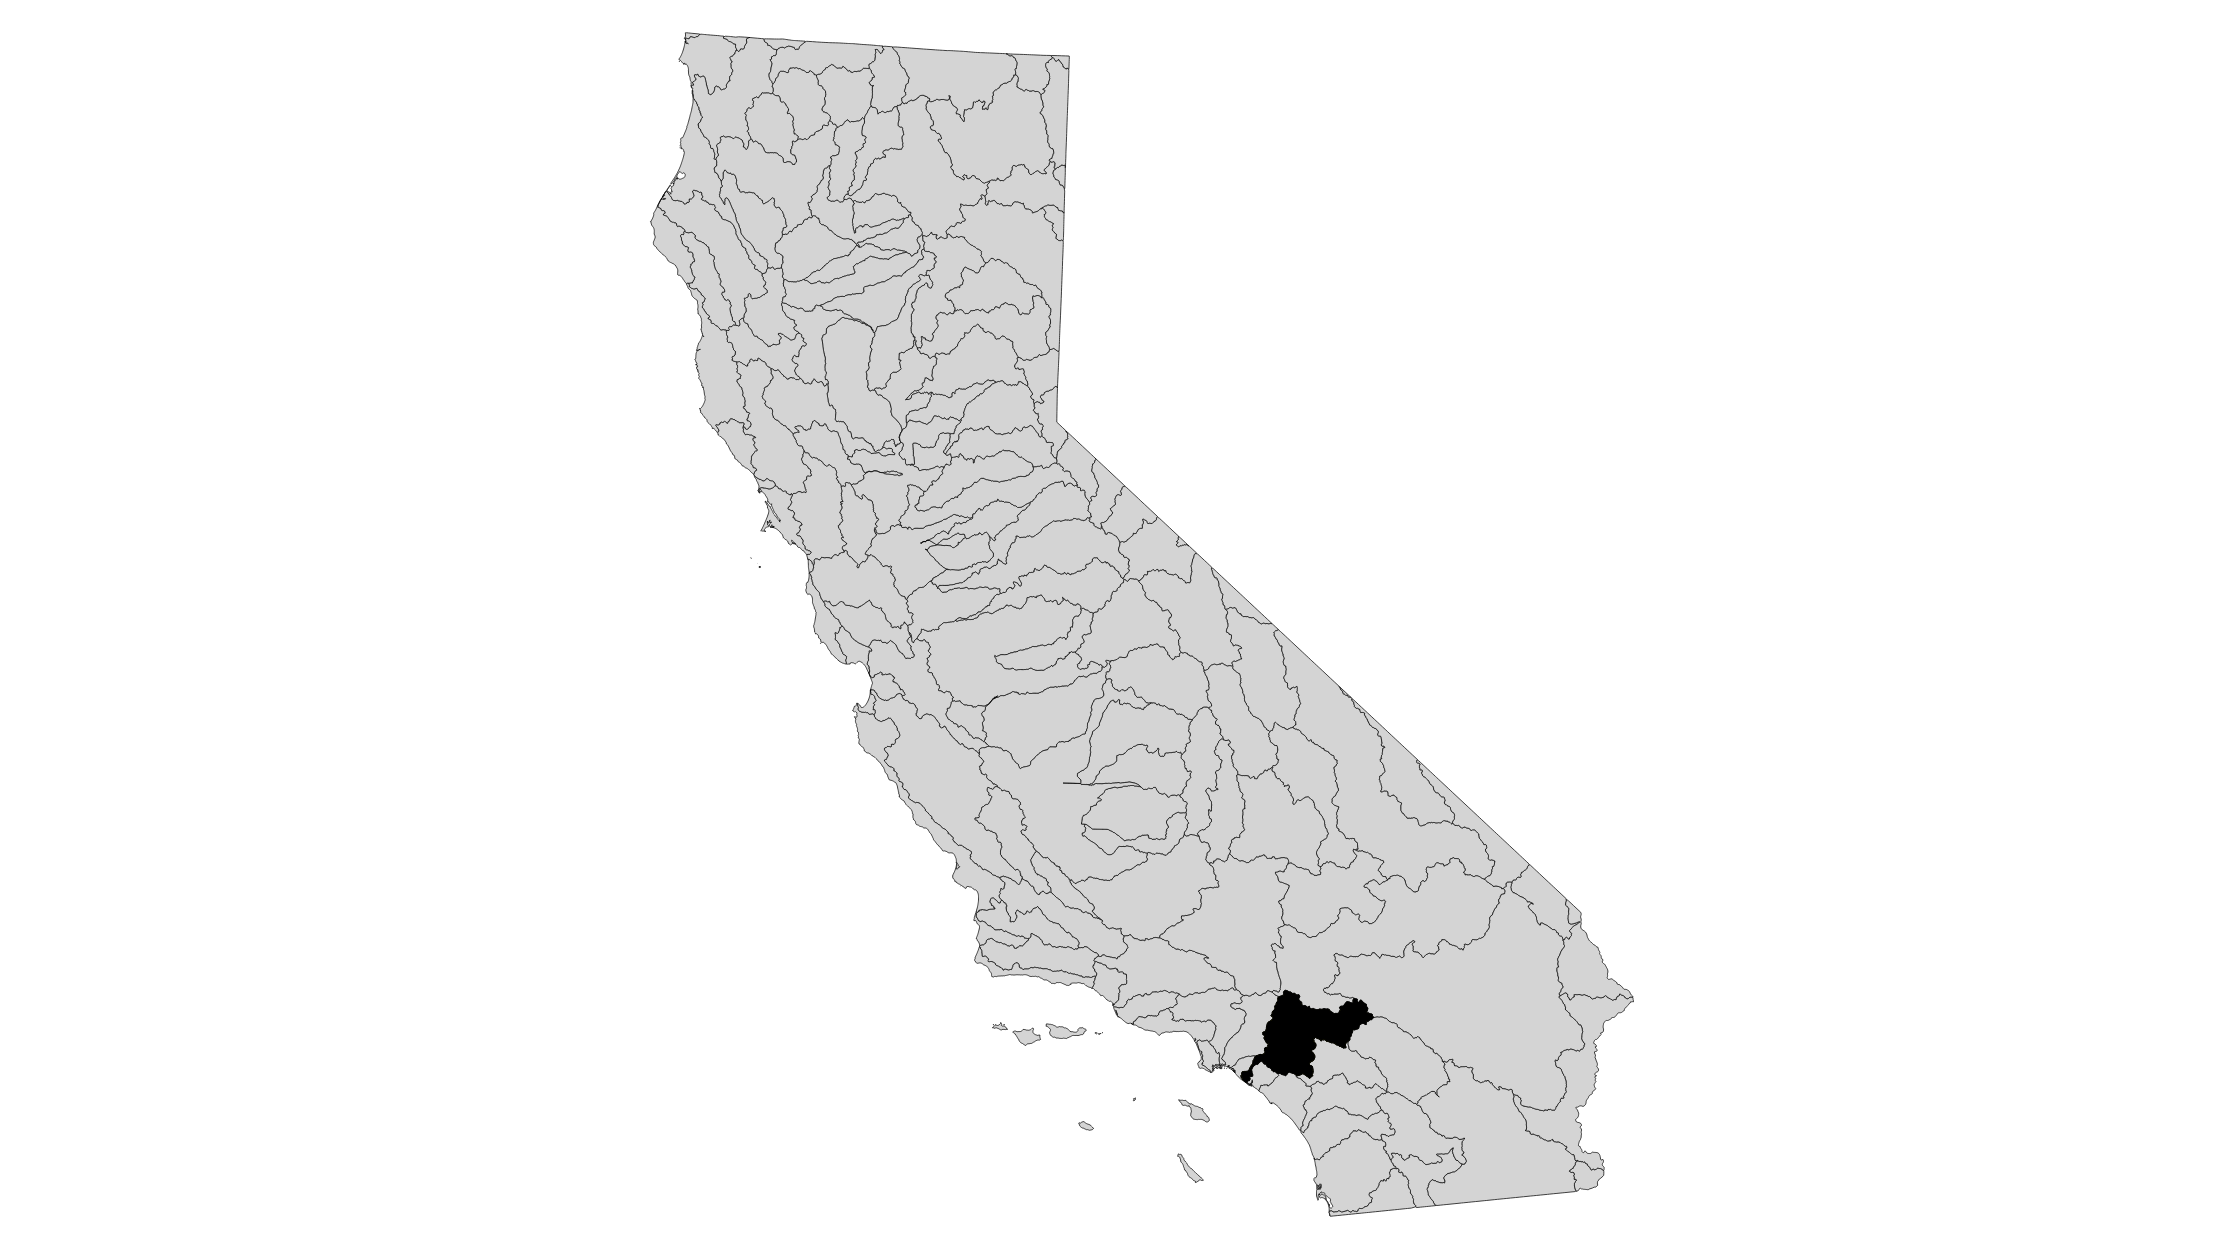
\includegraphics[width=5.5in]{figures/SanBernadino_Overview.png}   
            \caption{Santa Ana -- San Bernadino Region Overview (Filled in Black)}
            \label{fig:SASBoverview}
            \end{center}
        \end{figure}

    \subsection{Search Domain}
    
    \begin{itemize}
      \setlength{\itemsep}{0cm}
      \setlength{\parskip}{0cm}
        \item Grid Dimensions: $854$ $cells$ x $1463$ $cells$
        \item Grid Cell Resolution: $100$ $m$ x $100$ $m$ ($1$ $ha$)
        \item Feasible Grid Cells: $537,587$ $cells$
    \end{itemize}
    
        \begin{figure}[!h]
            \begin{center}
            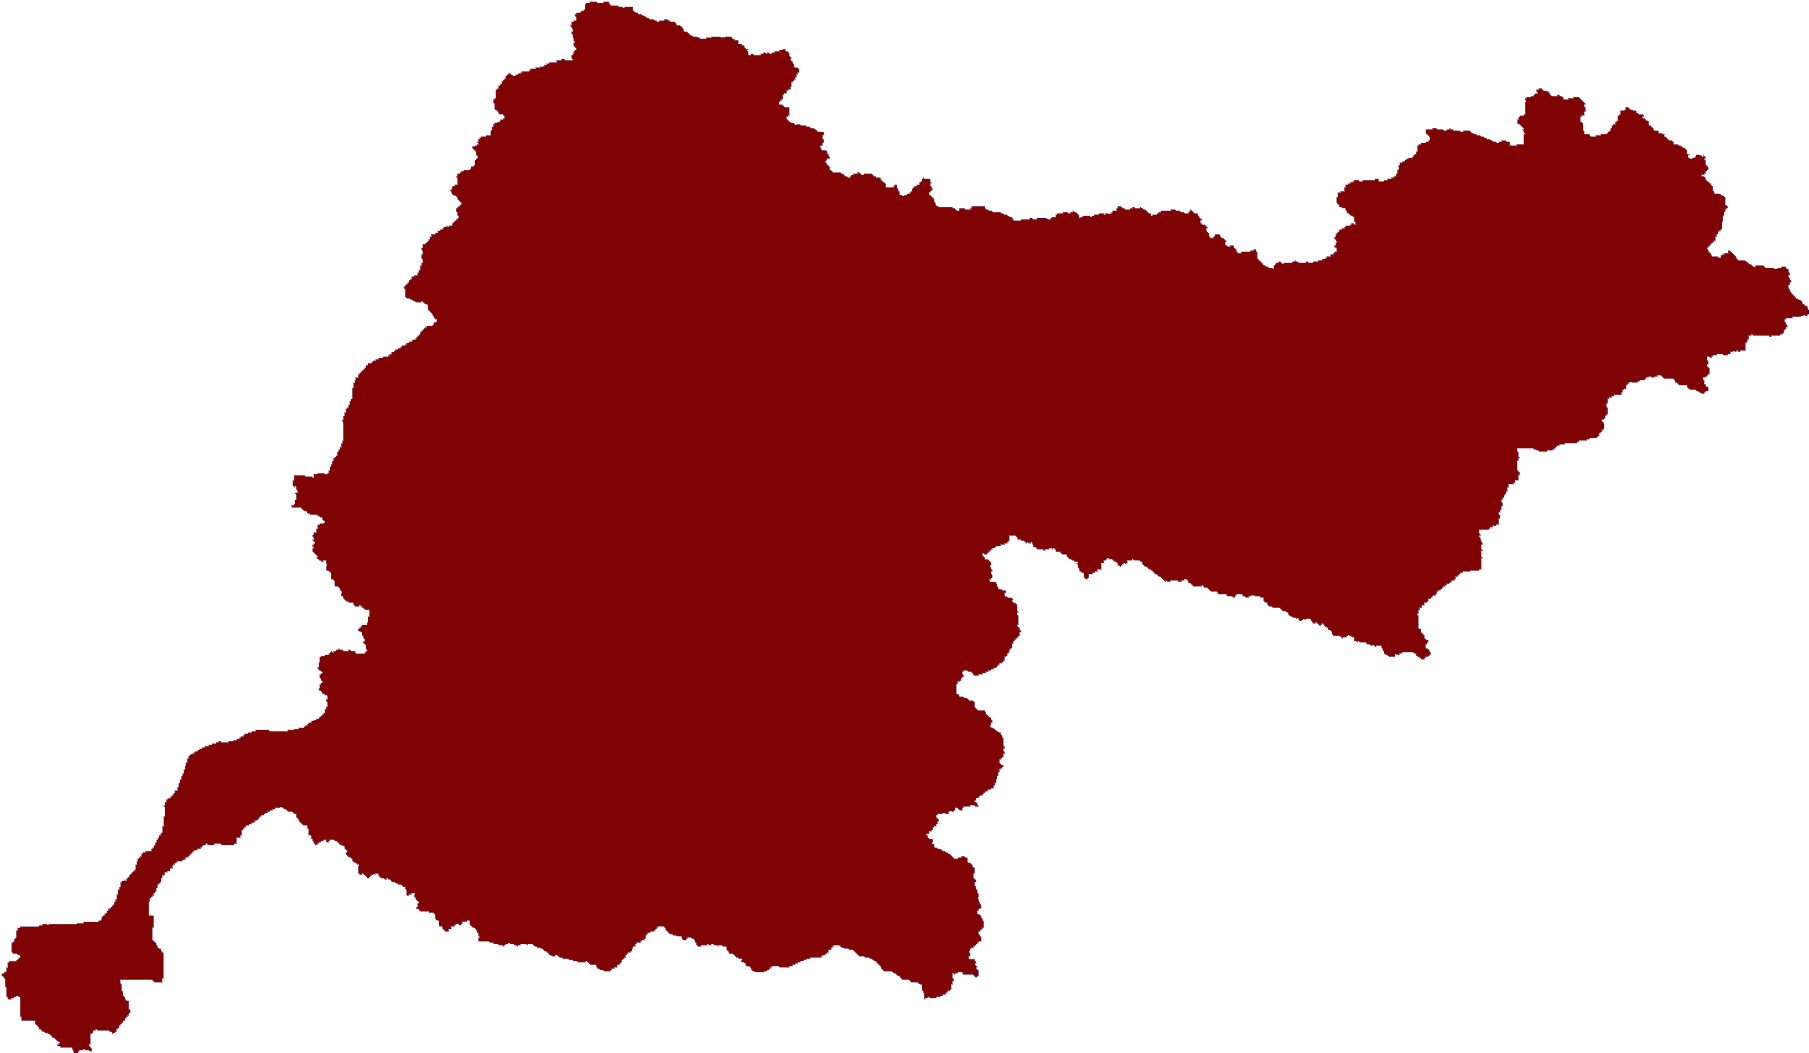
\includegraphics[width=5.5in]{figures/SanBernadino_SearchDomain.png}   
            \caption{Santa Ana -- San Bernadino Region Search Domain (Filled in Red)}
            \label{fig:SASBdomain}
            \end{center}
        \end{figure}
        
\subsection{Destination Search Inputs}
    
        \begin{figure}[!h]
            \begin{center}
            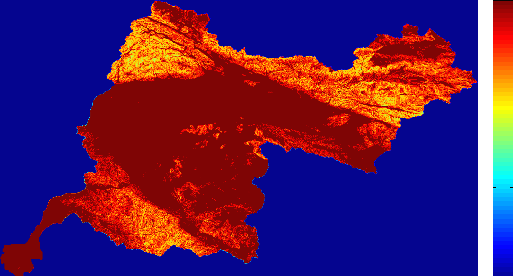
\includegraphics[width=5.5in]{figures/SanBernadino_Search_Slope.png}   
            \caption{Santa Ana -- San Bernadino Region Destination Search Inputs: Slope Score (Blue:Low, Red:High)}
            \label{fig:SASBdsinputs_slope}
            \end{center}
        \end{figure}
        
        \begin{figure}[!h]
            \begin{center}
            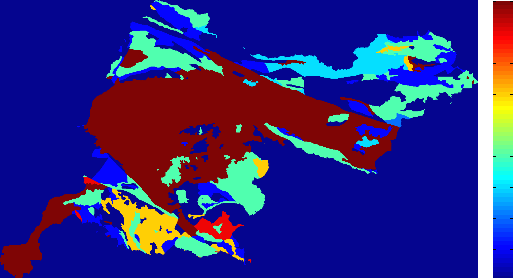
\includegraphics[width=5.5in]{figures/SanBernadino_Search_Geology.png}   
            \caption{Santa Ana -- San Bernadino Region Destination Search Inputs: Geology Score (Blue:Low, Red:High)}
            \label{fig:SASBdsinputs_geology}
            \end{center}
        \end{figure}
    
        \begin{figure}[!h]
            \begin{center}
            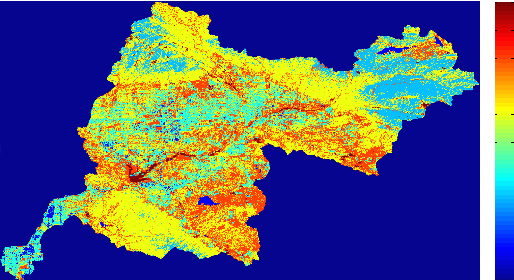
\includegraphics[width=5.5in]{figures/SanBernadino_Search_Landuse.png}   
            \caption{Santa Ana -- San Bernadino Region Destination Search Inputs: Landuse Score (Blue:Low, Red:High)}
            \label{fig:SASBdsinputs_landuse}
            \end{center}
        \end{figure}
    
    \subsection{Destination Search Outputs}
    
        \begin{figure}[!h]
            \begin{center}
            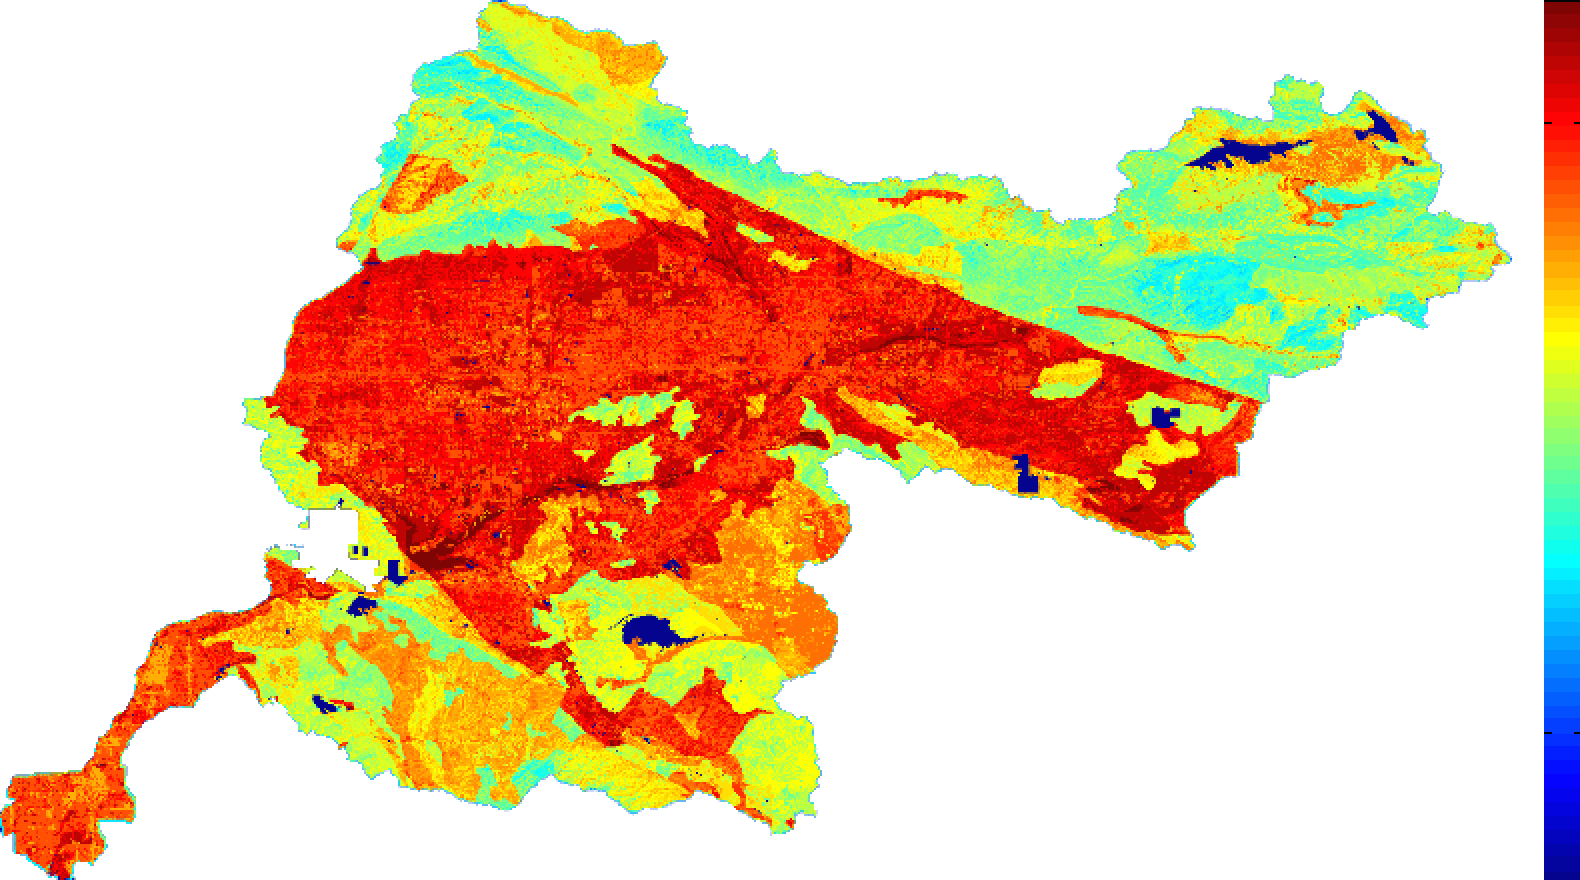
\includegraphics[width=5.5in]{figures/SanBernadino_Search_Composite.png}   
            \caption{Santa Ana -- San Bernadino Region Destination Search Outputs: Composite Scores (Blue:Low, Red:High)}
            \label{fig:SASBdsoutputs_comp}
            \end{center}
        \end{figure}
        
        \begin{figure}[!h]
            \begin{center}
            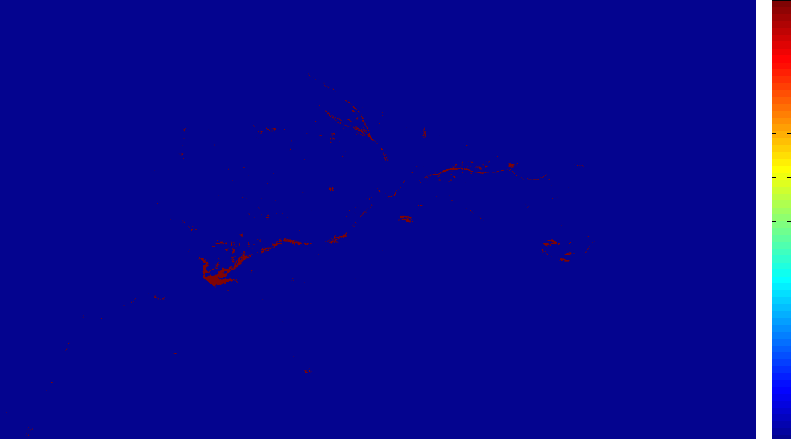
\includegraphics[width=5.5in]{figures/SanBernadino_Search_Output.png}   
            \caption{Santa Ana -- San Bernadino Region Destination Search Outputs: Candidate Regions}
            \label{fig:SASBdsoutputs_cand}
            \end{center}
        \end{figure}

    \subsection{Proposed Corridor Endpoints}
    
    \begin{itemize}
      \setlength{\itemsep}{0cm}
      \setlength{\parskip}{0cm}
        \item Start Location: $(840,48)$
        \item End Destination: 
        \item Shortest Euclidean Path Distance: 
    \end{itemize}
    
        \begin{figure}[!h]
            \begin{center}
            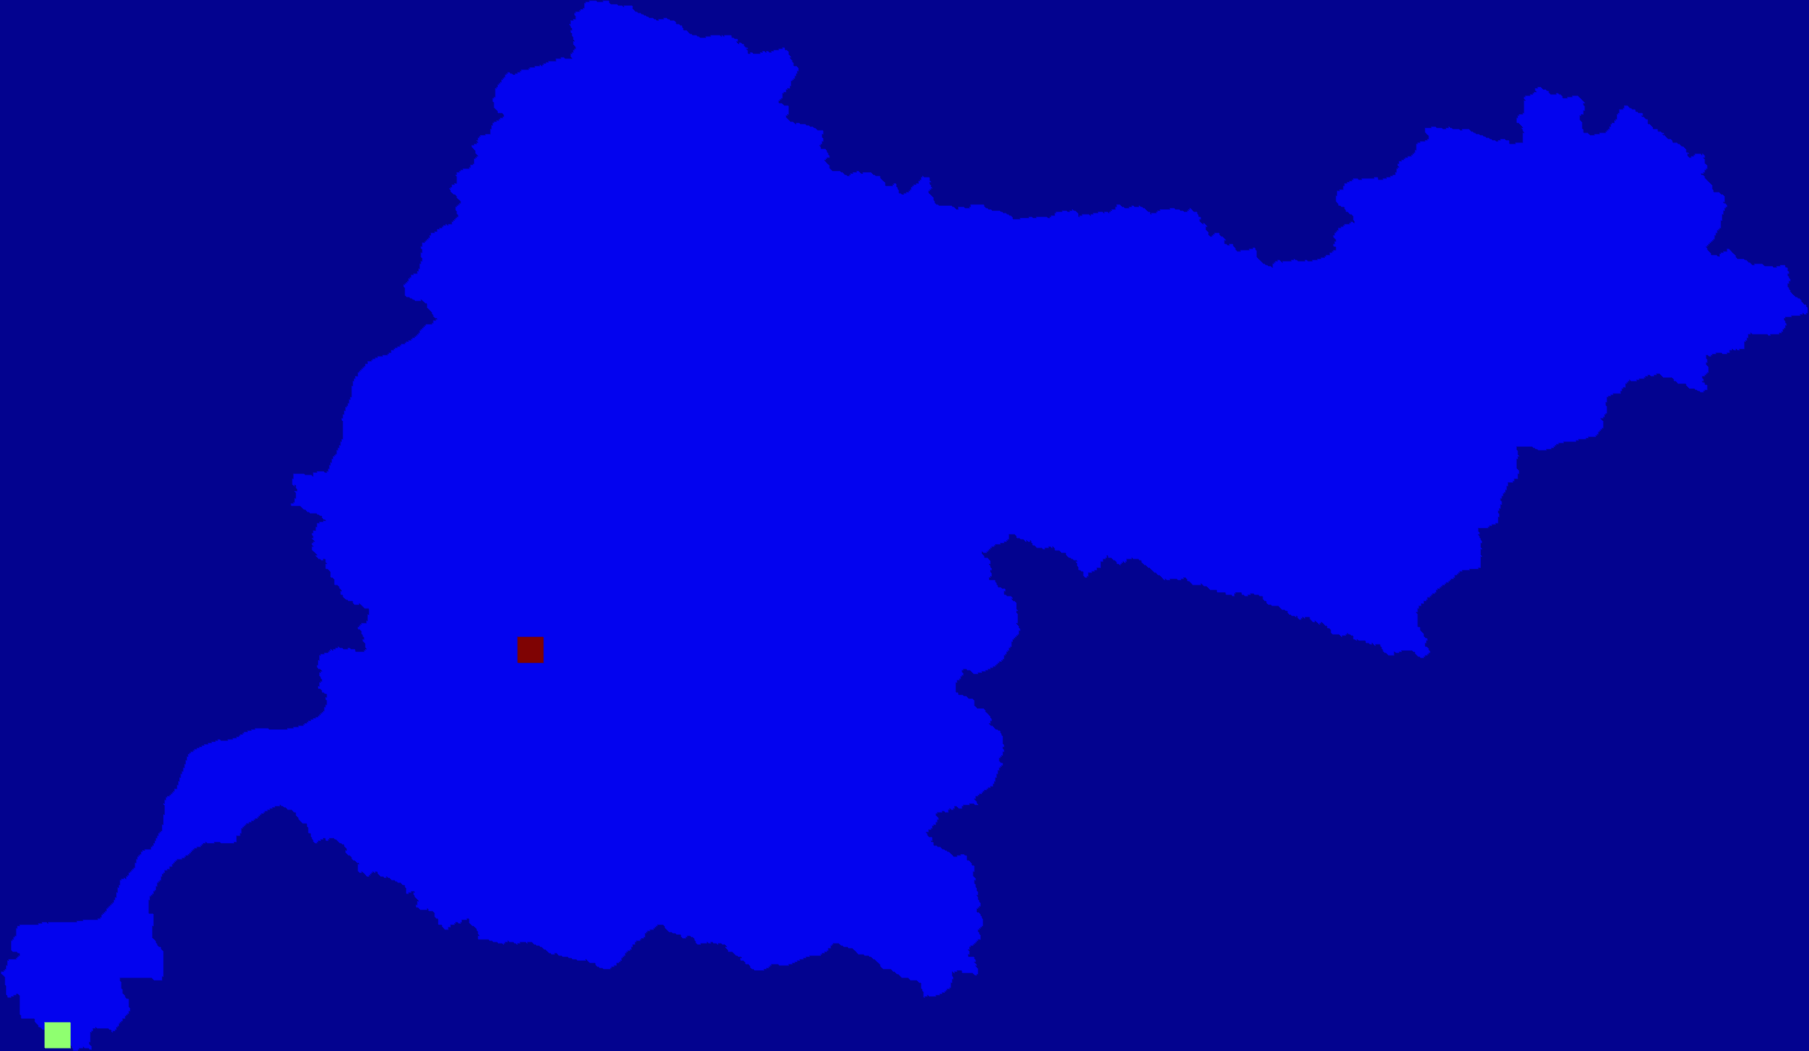
\includegraphics[width=5.5in]{figures/SanBernadino_Endpoints.png}   
            \caption{Santa Ana -- San Bernadino Region Proposed Corridor Endpoints}
            \label{fig:SASBendpoints}
            \end{center}
        \end{figure}
    
    \subsection{Proposed Objective Layers}

        \begin{figure}[!h]
            \begin{center}
            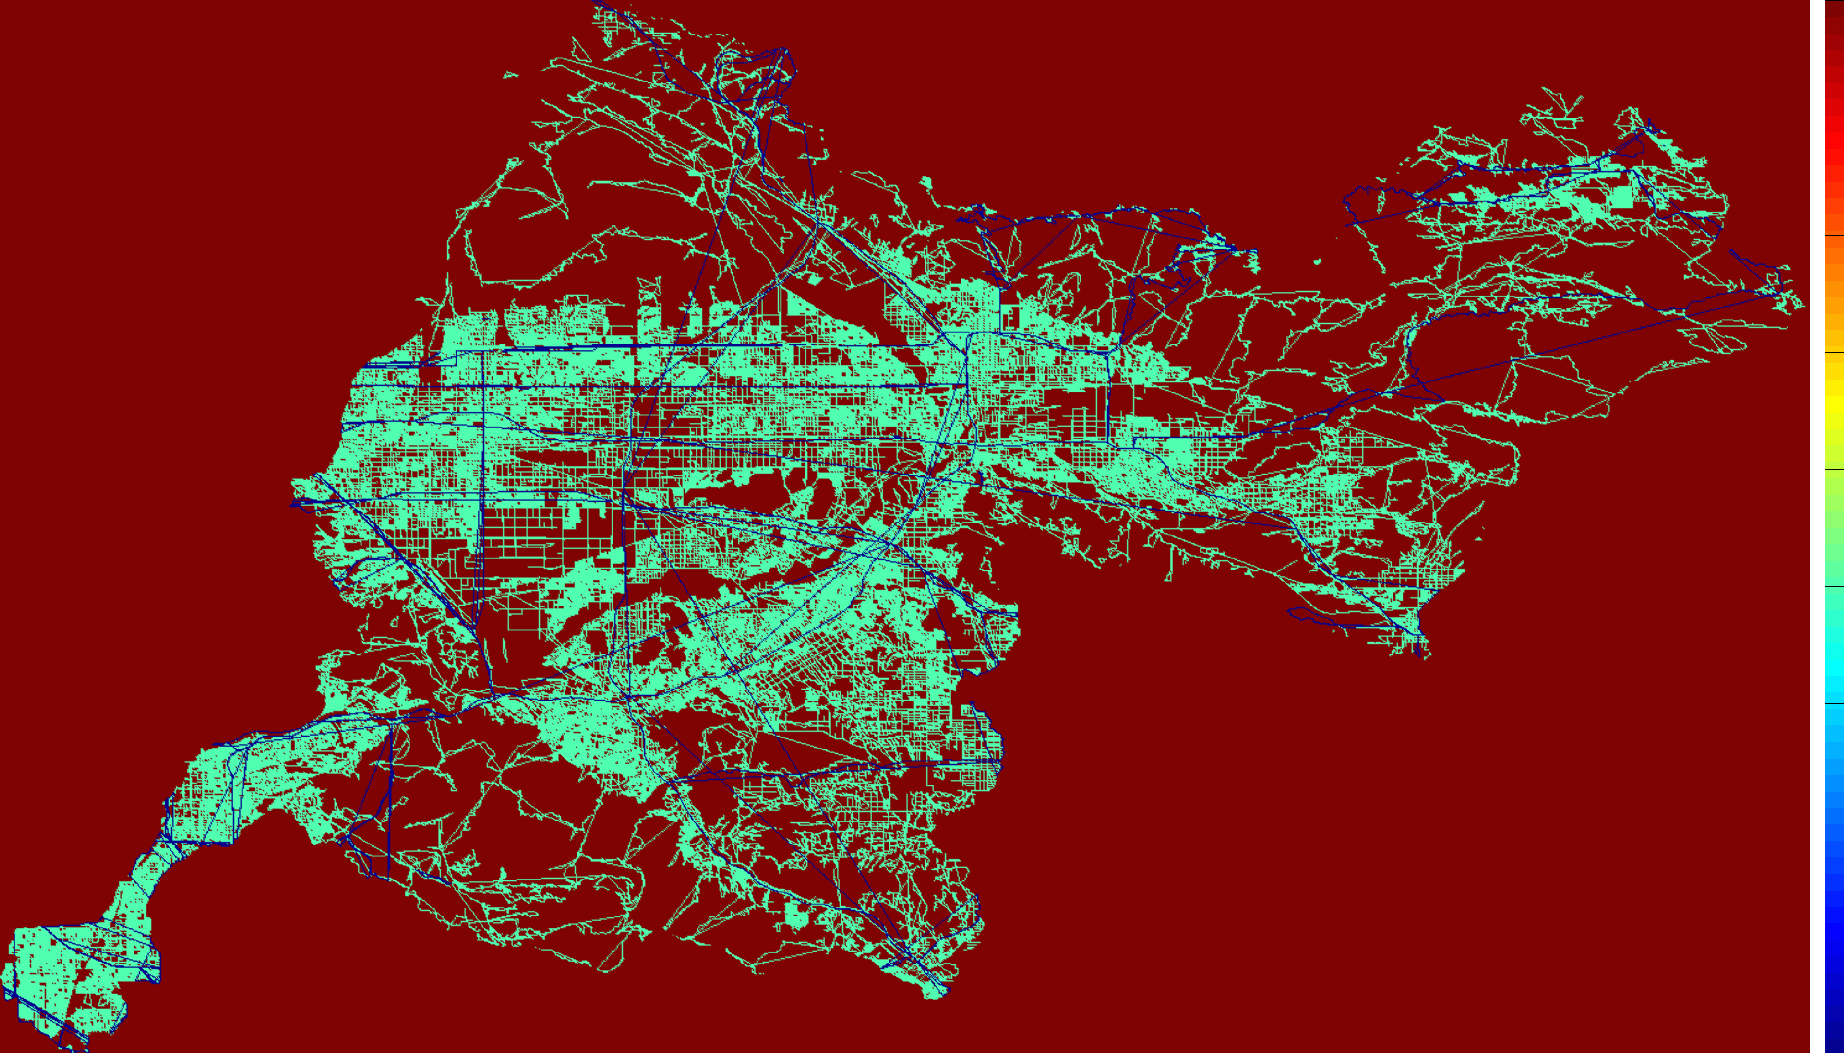
\includegraphics[width=5.5in]{figures/SanBernadino_AccessibilityScore.png}   
            \caption{Santa Ana -- San Bernadino Region Accessibility Based Objective Scores (Blue:Low, Red:High)}
            \label{fig:SASBaccessibilty}
            \end{center}
        \end{figure}

        \begin{figure}[!h]
            \begin{center}
            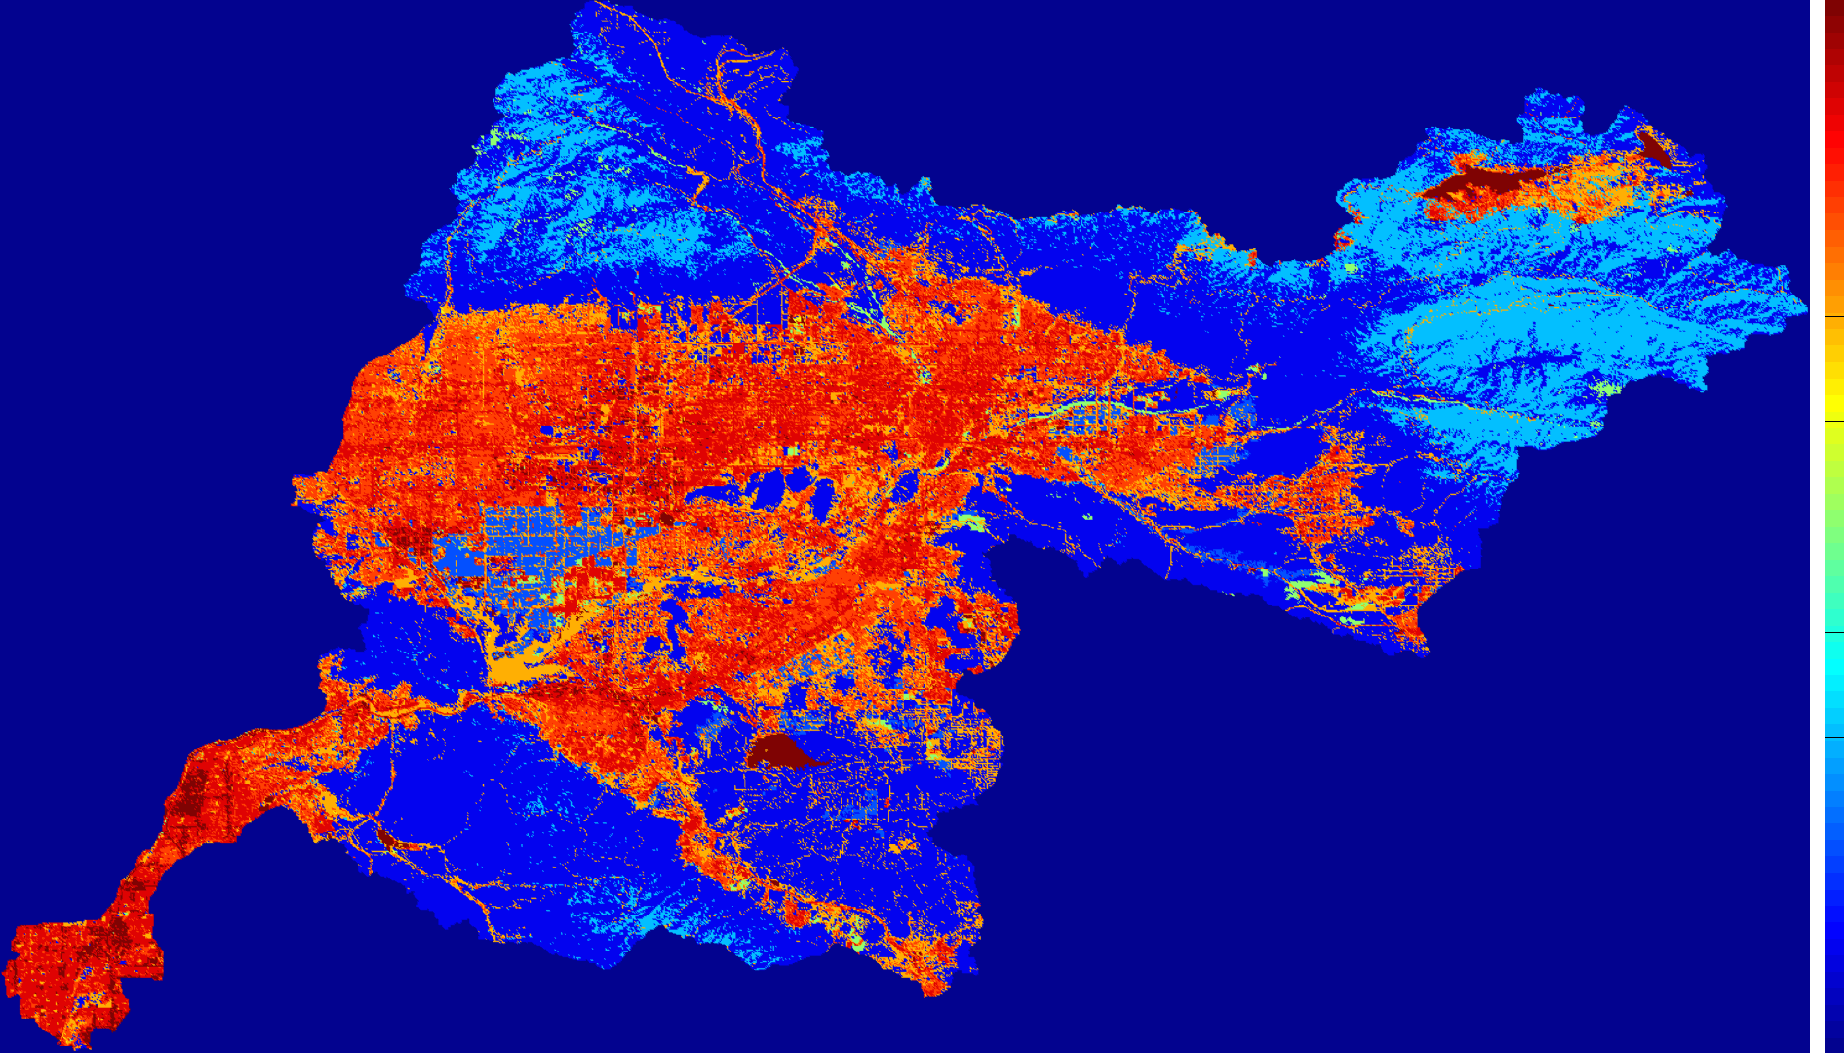
\includegraphics[width=5.5in]{figures/SanBernadino_DisturbanceScore.png}   
            \caption{Santa Ana -- San Bernadino Region Land Use Disturbance Based Objective Scores (Blue:Low, Red:High)}
            \label{fig:SASBdisturbance}
            \end{center}
        \end{figure}
        
        \begin{figure}[!h]
            \begin{center}
            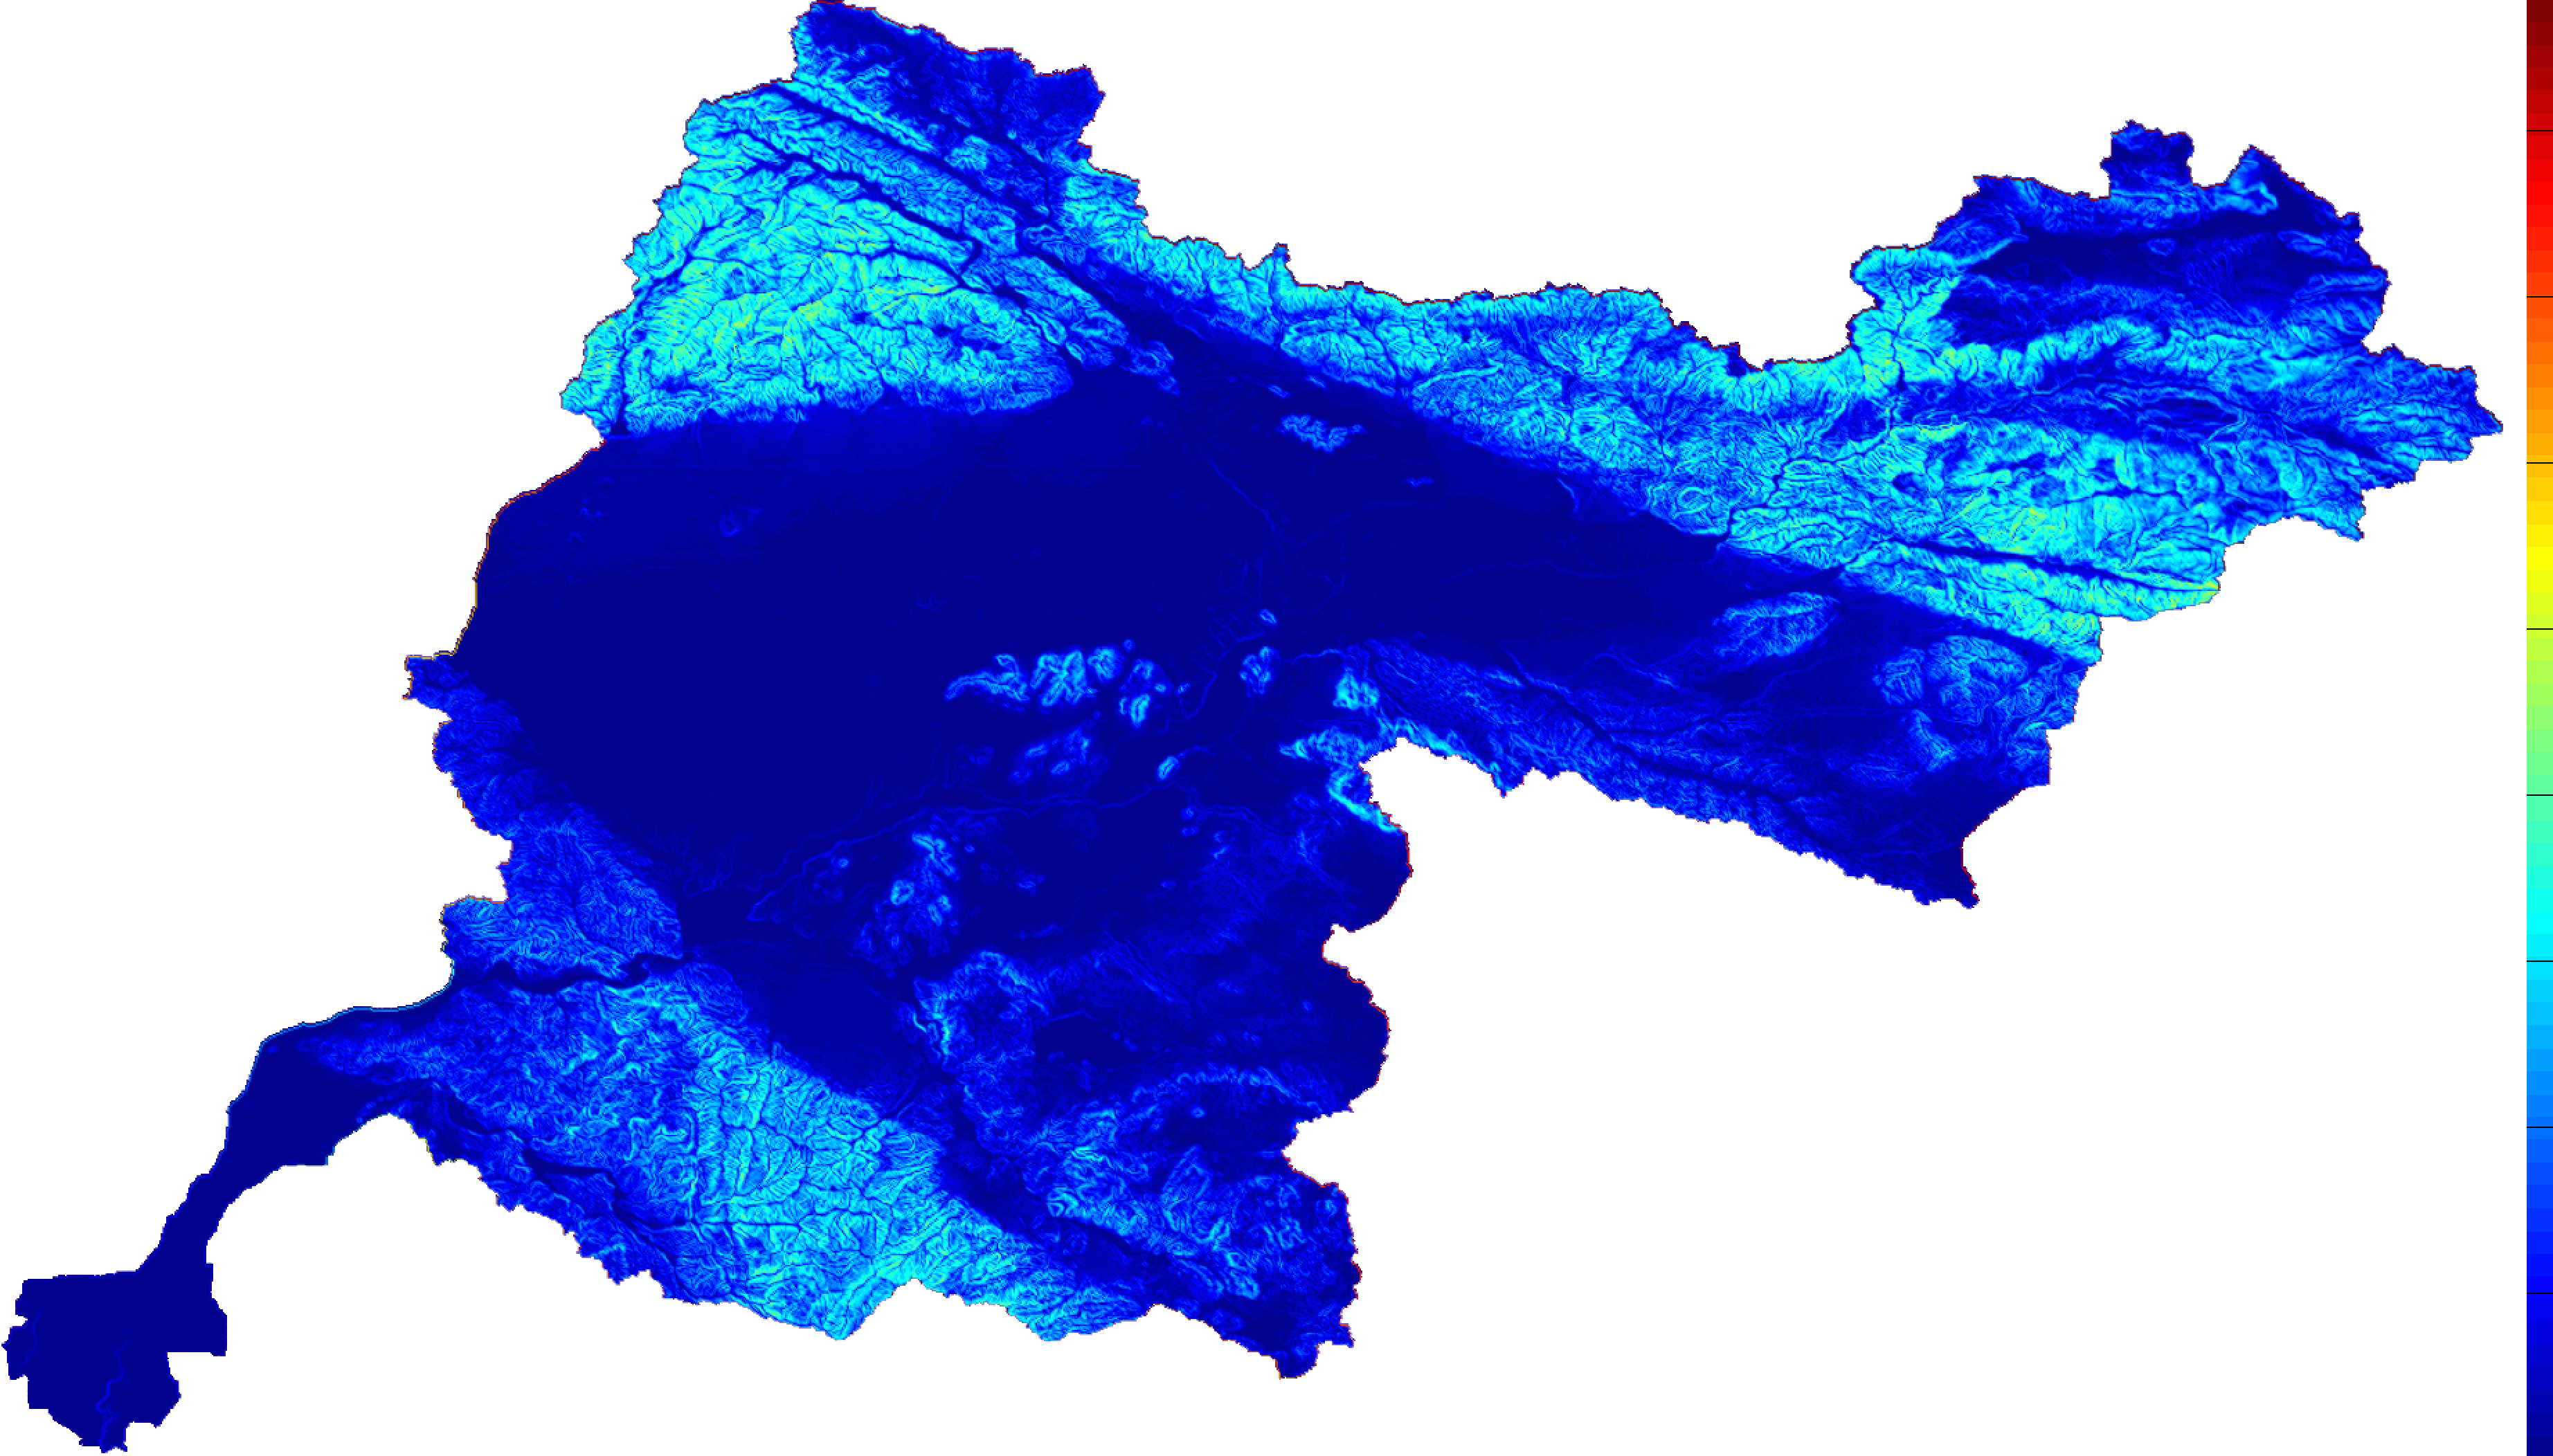
\includegraphics[width=5.5in]{figures/SanBernadino_SlopeScore.png}   
            \caption{Santa Ana -- San Bernadino Region Slope Based Objective Scores (Blue:Low, Red:High)}
            \label{fig:SASBslope}
            \end{center}
        \end{figure}
        
    \subsection{Proposed Corridor Solutions}
    
        \begin{figure}[!h]
            \begin{center}
            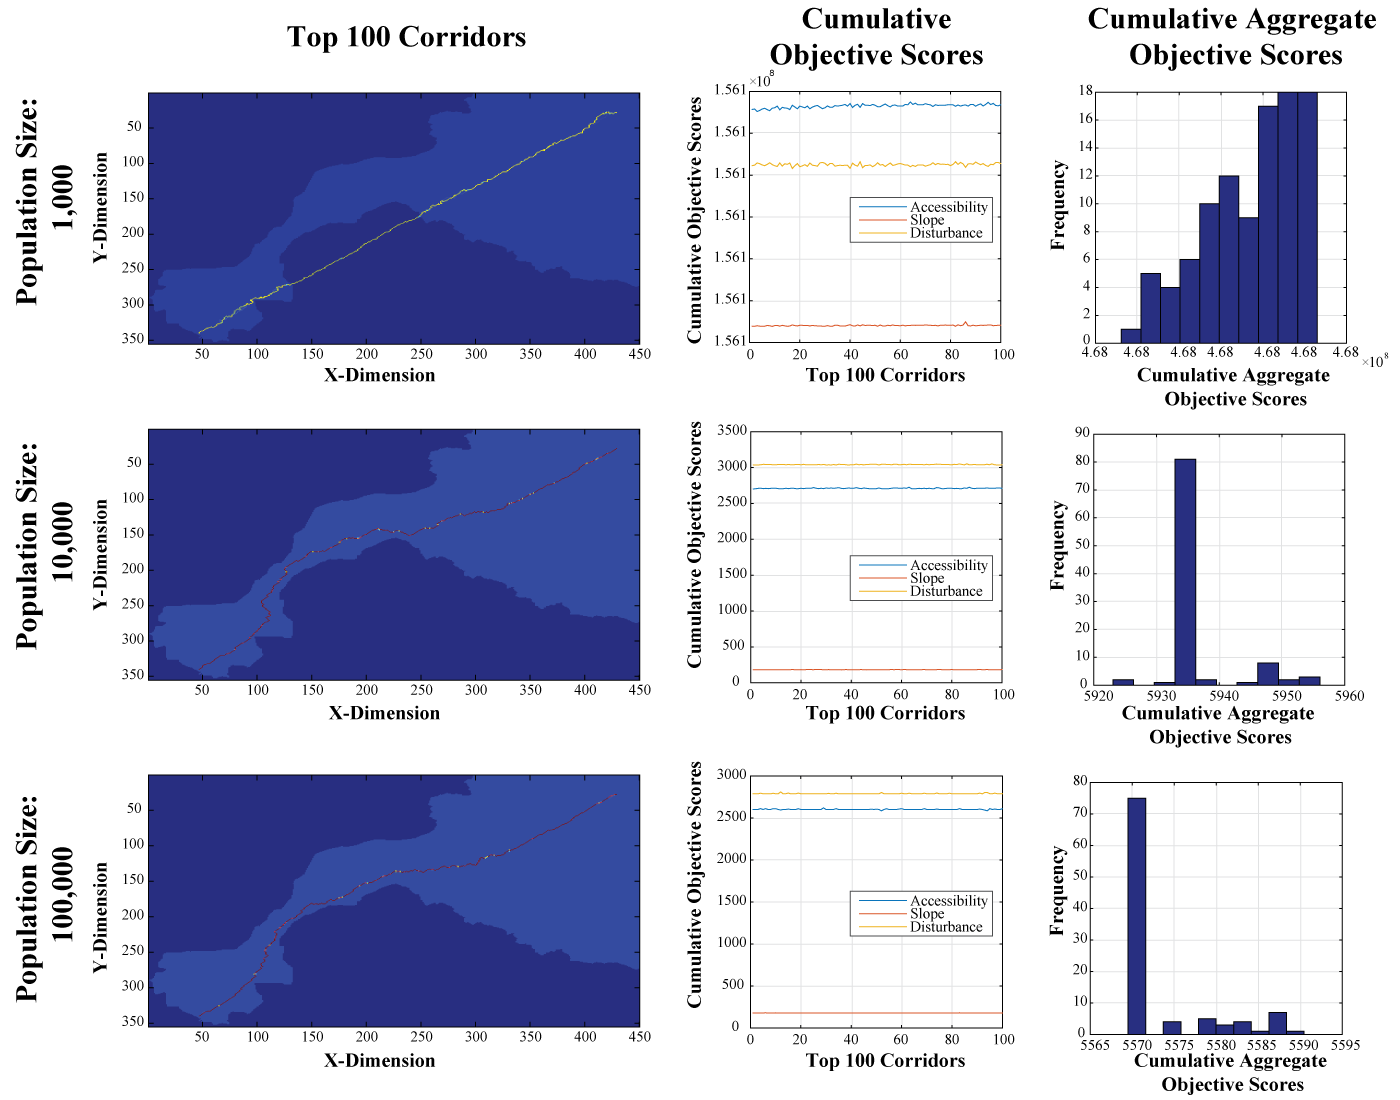
\includegraphics[width=6in]{figures/SanBernadino_PathwayResults.png}   
            \caption{Santa Ana -- San Bernadino Region Corridor Analysis Results}
            \label{fig:SASBresults}
            \end{center}
        \end{figure}

        \begin{figure}[!h]
            \begin{center}
            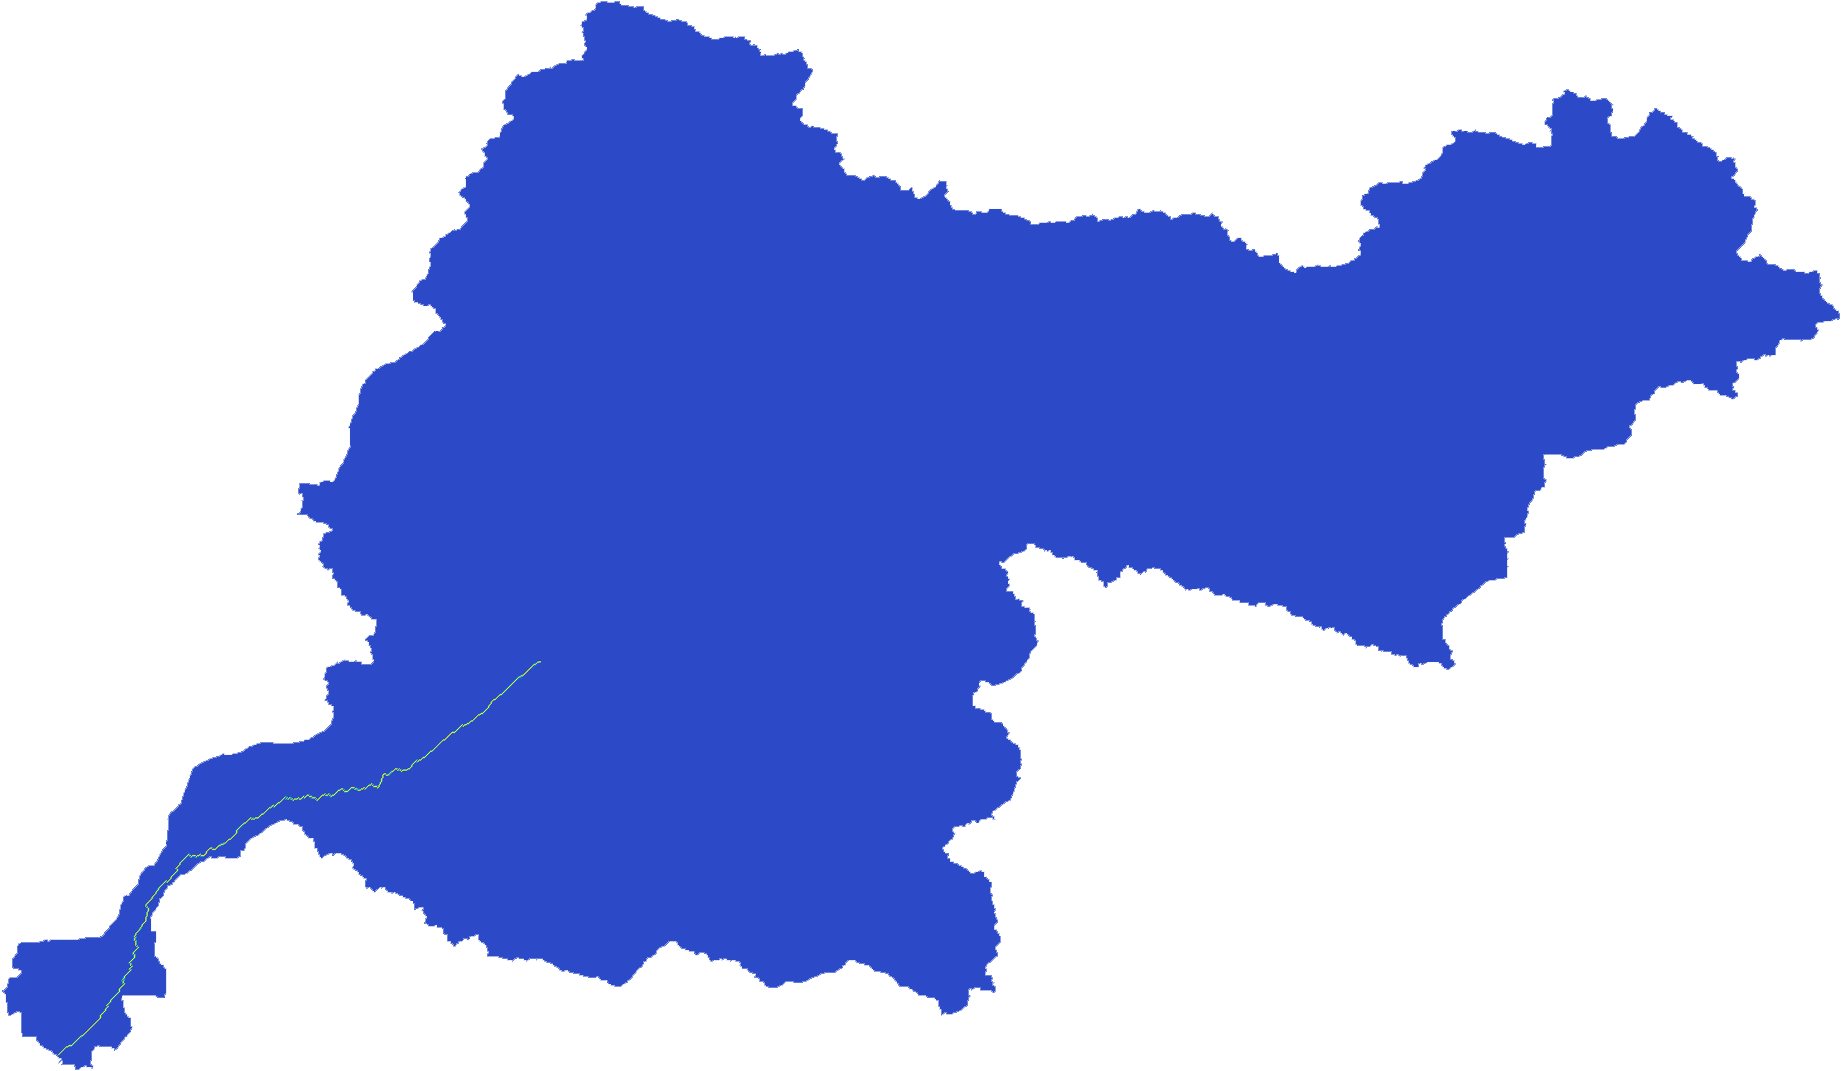
\includegraphics[width=5.5in]{figures/SanBernadino_PathwayLarge.png}   
            \caption{Santa Ana -- San Bernadino Region Top 100 Corridors (Pop Size: 100,000) Basin Wide Overview}
            \label{fig:SASBsolutionOverview}
            \end{center}
        \end{figure}
    
    \subsection{Anticipated Distribution of Life Cycle Energy Usages and Net Water Savings}

\section{Fresno -- Tulare Region}

    \subsection{Regional Context}

    \begin{itemize}
      \setlength{\itemsep}{0cm}
      \setlength{\parskip}{0cm}
        \item HUC-8 Code: $18030009$
        \item Total Area: $6,943.6$ $km^2$
        \item Maximum Elevation: $1,536.6$ $m$
        \item Minimum Elevation: $0$ $m$
        \item Mean Slope: $2.16$ $\%$
        \item Standard Deviation of Slope: $6.24$ $\%$
        \item Dominant Soil Composition: Hydrologic Soil Group - B: $10-20\%$ clay, $50-90\%$ sand, $35\%$ rock fragments
    \end{itemize}

        \begin{figure}[!h]
            \begin{center}
            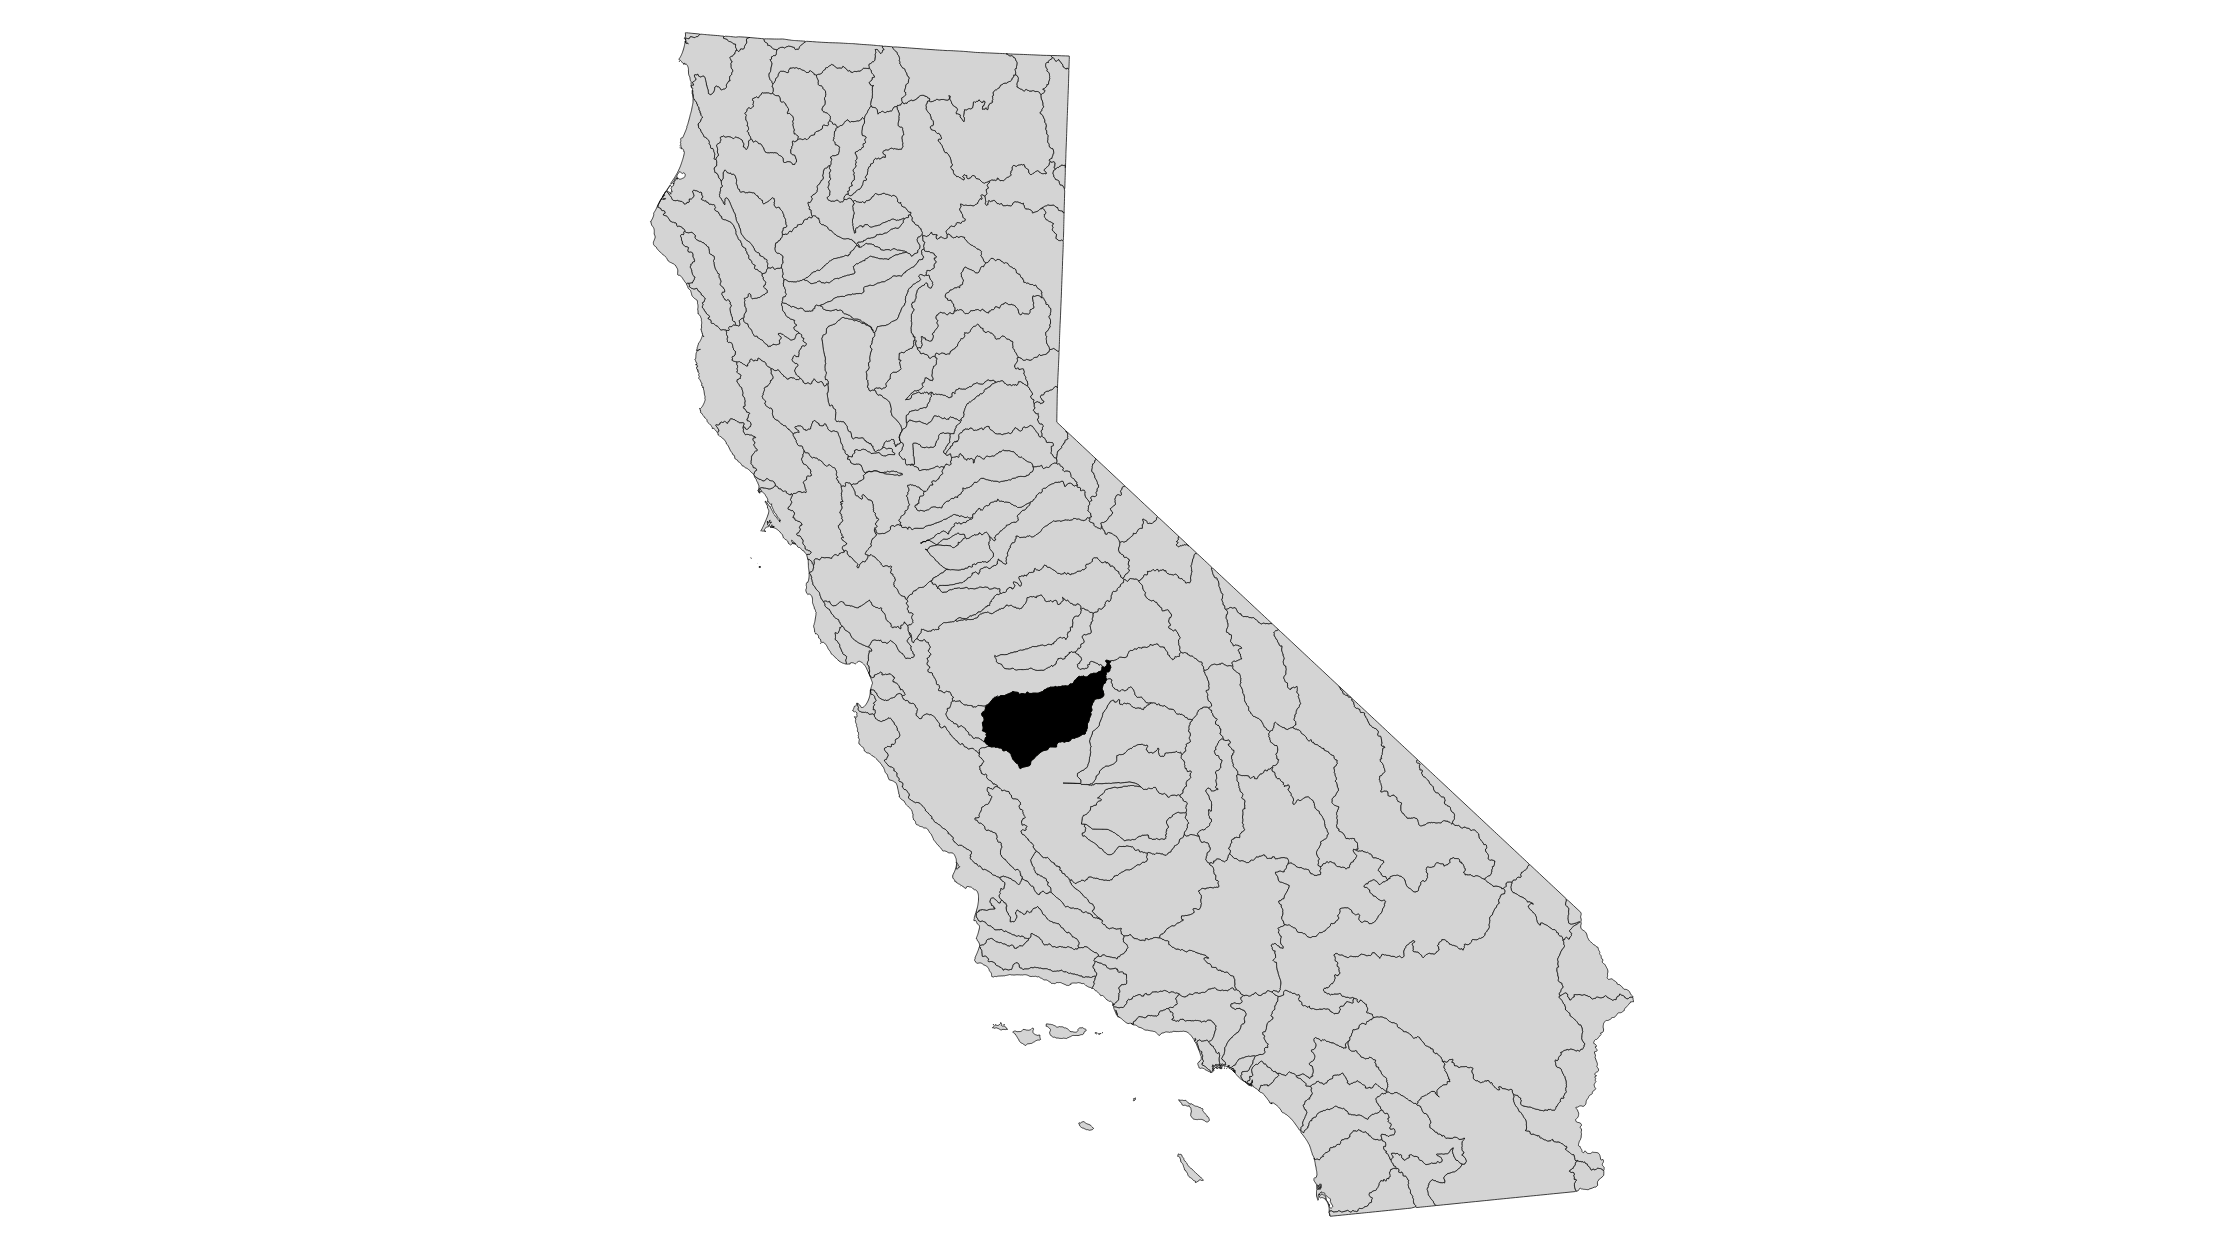
\includegraphics[width=5.5in]{figures/Fresno_Overview.png}   
            \caption{Fresno -- Tulare Region Overview (Filled in Black)}
            \label{fig:Foverview}
            \end{center}
        \end{figure}

    \subsection{Search Domain}
    
    \begin{itemize}
      \setlength{\itemsep}{0cm}
      \setlength{\parskip}{0cm}
        \item Grid Dimensions: $1018$ $cells$ x $1459$ $cells$
        \item Grid Cell Resolution: $100$ $m$ x $100$ $m$ ($1$ $ha$)
        \item Feasible Grid Cells: $694,365$ $cells$
    \end{itemize}
    
        \begin{figure}[!h]
            \begin{center}
            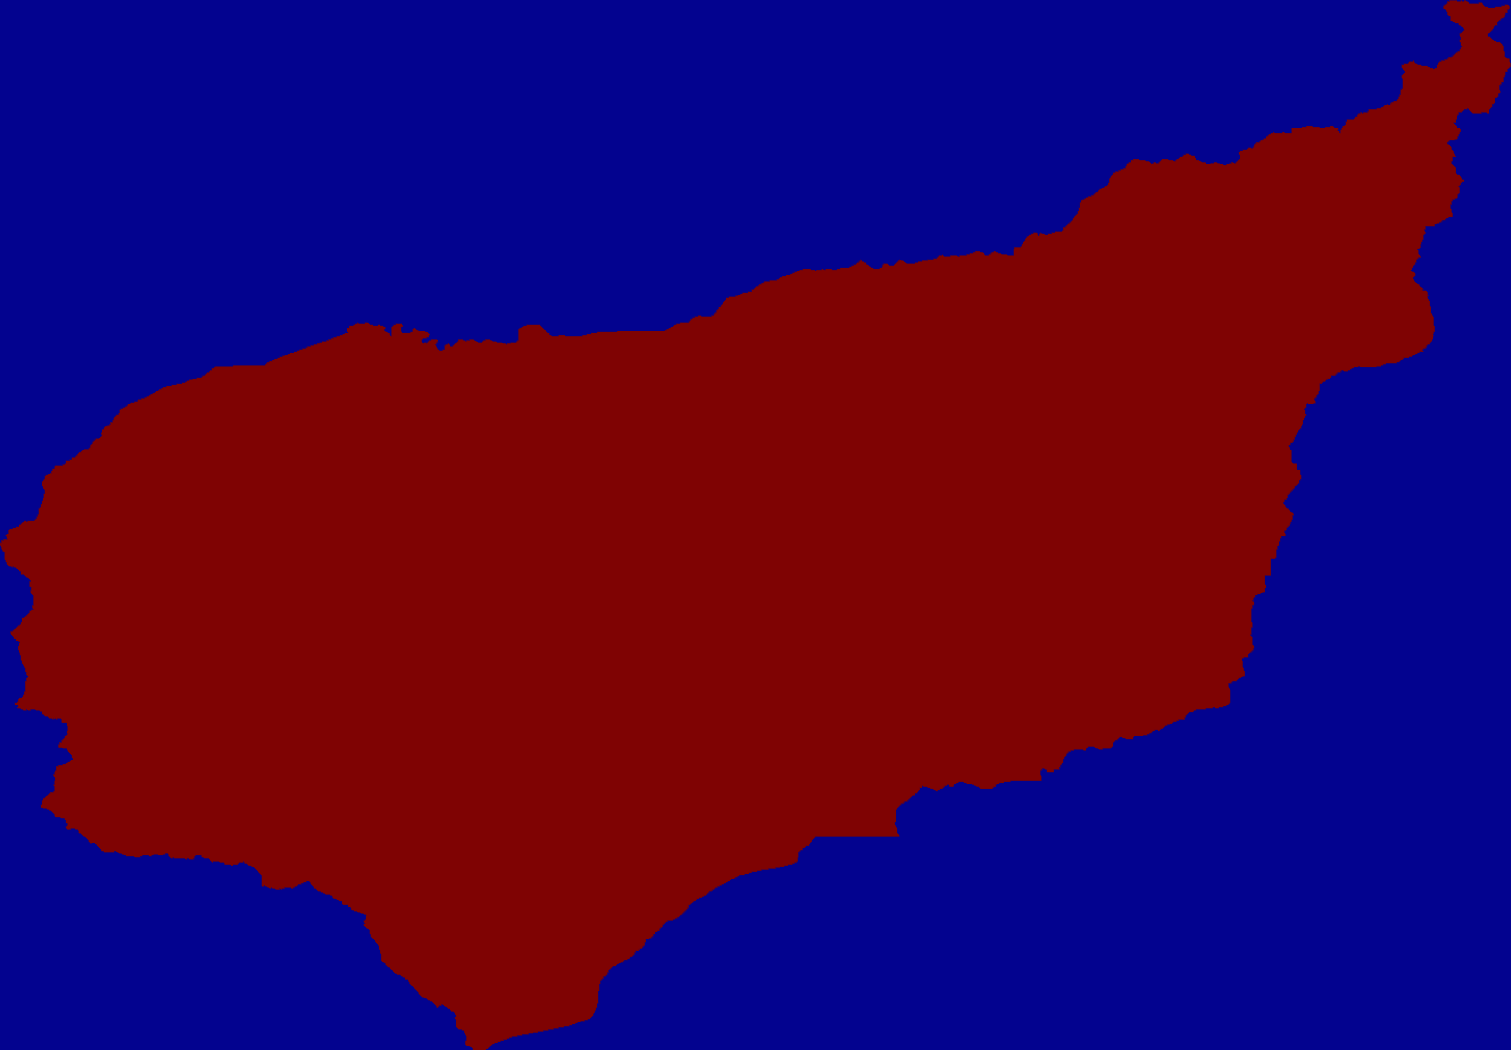
\includegraphics[width=5.5in]{figures/Fresno_SearchDomain.png}   
            \caption{Fresno -- Tulare Region Search Domain (Filled in Red)}
            \label{fig:Fdomain}
            \end{center}
        \end{figure}
        
    \subsection{Destination Search Inputs}
    
        \begin{figure}[!h]
            \begin{center}
            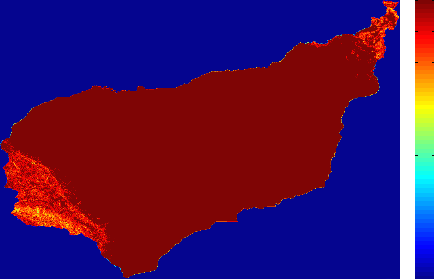
\includegraphics[width=5.5in]{figures/Fresno_Search_Slope.png}   
            \caption{Fresno -- Tulare Region Destination Search Inputs: Slope Score (Blue:Low, Red:High)}
            \label{fig:Fdsinputs_slope}
            \end{center}
        \end{figure}
        
        \begin{figure}[!h]
            \begin{center}
            \includegraphics[width=5.5in]{figures/Fresno_Search_Geology.png}   
            \caption{Fresno -- Tulare Region Destination Search Inputs: Geology Score (Blue:Low, Red:High)}
            \label{fig:Fdsinputs_geology}
            \end{center}
        \end{figure}
    
        \begin{figure}[!h]
            \begin{center}
            \includegraphics[width=5.5in]{figures/Fresno_Search_Landuse.png}   
            \caption{Fresno -- Tulare Region Destination Search Inputs: Landuse Score (Blue:Low, Red:High)}
            \label{fig:Fdsinputs_landuse}
            \end{center}
        \end{figure}
    
    \subsection{Destination Search Outputs}
    
        \begin{figure}[!h]
            \begin{center}
            \includegraphics[width=5.5in]{figures/Fresno_Search_Composite.png}   
            \caption{Fresno -- Tulare Region Destination Search Outputs: Composite Scores (Blue:Low, Red:High)}
            \label{fig:Fdsoutputs_comp}
            \end{center}
        \end{figure}
        
        \begin{figure}[!h]
            \begin{center}
            \includegraphics[width=5.5in]{figures/Fresno_Search_Output.png}   
            \caption{Fresno -- Tulare Region Destination Search Outputs: Candidate Regions}
            \label{fig:Fdsoutputs_cand}
            \end{center}
        \end{figure}

    \subsection{Proposed Corridor Endpoints}
    
    \begin{itemize}
      \setlength{\itemsep}{0cm}
      \setlength{\parskip}{0cm}
        \item Start Location: $(435,1037)$
        \item End Destination: 
        \item Shortest Euclidean Path Distance: 
    \end{itemize}
    
        \begin{figure}[!h]
            \begin{center}
            \includegraphics[width=5.5in]{figures/Fresno_Endpoints.png}   
            \caption{Fresno -- Tulare Region Proposed Corridor Endpoints}
            \label{fig:Fendpoints}
            \end{center}
        \end{figure}

    \subsection{Proposed Objective Layers}
    
        \begin{figure}[!h]
            \begin{center}
            \includegraphics[width=5.5in]{figures/Fresno_AccessibilityScore.png}   
            \caption{Fresno -- Tulare Region Accessibility Based Objective Scores (Blue:Low, Red:High)}
            \label{fig:Faccessibilty}
            \end{center}
        \end{figure}

        \begin{figure}[!h]
            \begin{center}
            \includegraphics[width=5.5in]{figures/Fresno_DisturbanceScore.png}   
            \caption{Fresno -- Tulare Region Land Use Disturbance Based Objective Scores (Blue:Low, Red:High)}
            \label{fig:Fdisturbance}
            \end{center}
        \end{figure}
        
        \begin{figure}[!h]
            \begin{center}
            \includegraphics[width=5.5in]{figures/Fresno_SlopeScore.png}   
            \caption{Fresno -- Tulare Region Slope Based Objective Scores (Blue:Low, Red:High)}
            \label{fig:Fslope}
            \end{center}
        \end{figure}
        
    \subsection{Proposed Corridor Solutions}
    
        \begin{figure}[!h]
            \begin{center}
            \includegraphics[width=6in]{figures/Fresno_PathwayResults.png}   
            \caption{Fresno Region Corridor Analysis Results}
            \label{fig:Fresults}
            \end{center}
        \end{figure}

        \begin{figure}[!h]
            \begin{center}
            \includegraphics[width=5.5in]{figures/Fresno_PathwayLarge.png}   
            \caption{Fresno Region Top 100 Corridors (Pop Size: 100,000) Basin Wide Overview}
            \label{fig:FsolutionOverview}
            \end{center}
        \end{figure}
        
    \subsection{Anticipated Distribution of Life Cycle Energy Usages and Net Water Savings}
        
\section{Algorithm Runtime Performance}

    \begin{figure}[!h]
        \begin{center}
        \includegraphics[width=5.5in]{figures/Runtimes.png}
        \caption{Algorithm Runtime Performance for Each of the Five Case Study Regions for Three Population Sizes}
        \label{fig:Runtimes}
        \end{center}
    \end{figure}
    
    \begin{figure}[!h]
        \begin{center}
        \includegraphics[width=5.5in]{figures/Evolutions.png}
        \caption{Algorithm Convergence Rates for Each of the Five Case Study Regions for Three Population Sizes}
        \label{fig:Evolutions}
        \end{center}
    \end{figure}

\section{Solution Quality Evaluation}

    \begin{figure}[!h]
        \begin{center}
        \includegraphics[width=5.5in]{figures/Margin_Improvement.png}
        \caption{Comparison of the Along Path Distance and Cumulative Objective Scores between the Solution Corridors and the Euclidean Shortest Corridors}
        \label{fig:MarginImprovement}
        \end{center}
    \end{figure}
